%%%%%%%%%%%%%%%%%%%%%%%%%%%%%%%%%%%%%%%%%%%%%%%%%%%%%%%%%%%%%%%%%%%%%%%%%%%%%%%%
%%%%%%%%%%%%%%%%%%   Vorlage für eine Abschlussarbeit   %%%%%%%%%%%%%%%%%%%%%%%%
%%%%%%%%%%%%%%%%%%%%%%%%%%%%%%%%%%%%%%%%%%%%%%%%%%%%%%%%%%%%%%%%%%%%%%%%%%%%%%%%

% Erstellt von Maximilian Nöthe, <maximilian.noethe@tu-dortmund.de>
% ausgelegt für lualatex und Biblatex mit biber

% Kompilieren mit 
% lualatex dateiname.tex
% biber dateiname.bcf
% lualatex dateiname.tex
% lualatex dateiname.tex
% oder einfach mit:
% make

\documentclass[
  BCOR=12mm,     % 12mm binding corrections, adjust to fit your binding
  parskip=half,  % new paragraphs start with half line vertical space
  open=any,      % chapters start on both odd and even pages
  cleardoublepage=plain,  % no header/footer on blank pages
]{tudothesis}


% Warning, if another latex run is needed
\usepackage[aux]{rerunfilecheck}

% just list chapters, sections and subsections in the toc, not subsubsection or smaller
\setcounter{tocdepth}{2}

%------------------------------------------------------------------------------
%------------------------------ Sprache und Schrift: --------------------------
%------------------------------------------------------------------------------
\usepackage{fontspec}
\defaultfontfeatures{Ligatures=TeX}  % -- becomes en-dash etc.

% german language
\usepackage{polyglossia}
\setdefaultlanguage{german}

% for english abstract and english titles in the toc
\setotherlanguages{english}

% intelligent quotation marks, language and nesting sensitive
\usepackage[autostyle]{csquotes}

% microtypographical features, makes the text look nicer on the small scale
\usepackage{microtype}

%------------------------------------------------------------------------------
%------------------------ Für die Matheumgebung--------------------------------
%------------------------------------------------------------------------------

\usepackage{amsmath}
\usepackage{amssymb}
\usepackage{mathtools}
\usepackage{upgreek}

% Enable Unicode-Math and follow the ISO-Standards for typesetting math
\usepackage[
  math-style=ISO,
  bold-style=ISO,
  sans-style=italic,
  nabla=upright,
  partial=upright,
]{unicode-math}
\setmathfont{Latin Modern Math}

% nice, small fracs for the text with \sfrac{}{}
\usepackage{xfrac}  


%------------------------------------------------------------------------------
%---------------------------- Numbers and Units -------------------------------
%------------------------------------------------------------------------------

\usepackage[
  locale=DE,
  separate-uncertainty=true,
  output-decimal-marker = {.},
  per-mode=symbol-or-fraction,
]{siunitx}
\sisetup{math-micro=\text{µ},text-micro=µ}

%------------------------------------------------------------------------------
%-------------------------------- tables  -------------------------------------
%------------------------------------------------------------------------------

\usepackage{booktabs}       % stellt \toprule, \midrule, \bottomrule

%------------------------------------------------------------------------------
%-------------------------------- graphics -------------------------------------
%------------------------------------------------------------------------------

\usepackage{graphicx}
\usepackage{grffile}

% allow figures to be placed in the running text by default:
\usepackage{scrhack}
\usepackage{float}
\floatplacement{figure}{htbp}
\floatplacement{table}{htbp}

% keep figures and tables in the section
\usepackage[section, below]{placeins}


%------------------------------------------------------------------------------
%---------------------- customize list environments ---------------------------
%------------------------------------------------------------------------------

\usepackage{enumitem}

%------------------------------------------------------------------------------
%------------------------------ Bibliographie ---------------------------------
%------------------------------------------------------------------------------

\usepackage[
backend=biber,   % use modern biber backend
autolang=hyphen, % load hyphenation rules for if language of bibentry is not
% german, has to be loaded with \setotherlanguages
% in the references.bib use langid={en} for english sources
bibstyle=phys_msc,
citestyle=phys_msc,
sorting=nyt
%style=phys
]{biblatex}
\addbibresource{references.bib}  % die Bibliographie einbinden
\DefineBibliographyStrings{german}{andothers = {{et\,al\adddot}}} 

%------------------------------------------------------------------------------
%------------------------------ Sonstiges: ------------------------------------
%------------------------------------------------------------------------------

\usepackage[pdfusetitle,unicode,linkbordercolor=tugreen]{hyperref}
\usepackage{bookmark}
\usepackage[shortcuts]{extdash}

\usepackage{listings}

\lstset{
	breaklines=true,
%	postbreak=\raisebox{0ex}[0ex][0ex]{\ensuremath{\color{red}\hookrightarrow\space}}
}

\usepackage{chemformula}


% Custom

\usepackage{rotating}
% \usepackage{mwe}
% \usepackage{subfig}
% \usepackage{lscape}

\newcommand*\circled[1]{\tikz[baseline=(char.base)]{
    \node[shape=circle,draw,inner sep=1pt] (char) {#1};}}

\newcommand{\myvec}[1]{\ensuremath{\begin{pmatrix}#1\end{pmatrix}}}
\usepackage{braket}

\usepackage{wrapfig}

%------------------------------------------------------------------------------
%-------------------------    Angaben zur Arbeit   ----------------------------
%------------------------------------------------------------------------------

\author{Jens Adam}
\title{TITEL}
\date{2018}
\birthplace{Bielefeld}
\chair{Lehrstuhl für Experimentelle Physik III}
\division{Fakultät Physik}
\thesisclass{Master of Science}
\submissiondate{23. April 2018}
\firstcorrector{Prof.~Dr.~Roland~Böhmer}
\secondcorrector{Priv.-Doz.~Dr.~Ute~Löw}

% tu logo on top of the titlepage
\titlehead{
\includegraphics[height=1.5cm]{logos/tu-logo.pdf}}

\begin{document}
\frontmatter
\maketitle

% Gutachterseite
\makecorrectorpage

% hier beginnt der Vorspann, nummeriert in römischen Zahlen
%\thispagestyle{plain}
\section*{}
\tableofcontents

\mainmatter
% Hier beginnt der Inhalt mit Seite 1 in arabischen Ziffern
\chapter{Einleitung}


Durch den immer weiter fortschreitenden Umstieg auf erneuerbare Energien, werden gute Möglichkeiten zur Speicherung der gewonnenen Energie zunehmend wichtiger -- dies resultiert in einem entsprechend hohen Forschungsinteresse. Ein Vorschlag für eine neue Technologie ist die Nutzung von ionische Flüssigkeiten. Um aber am Ende effiziente Produkte herstellen zu können, müssen die physikalischen Vorgänge auf mikroskopischer Ebene verstanden sein. Dies betrifft insbesondere die Struktur und Dynamik von Molekülen und Atomen. 

Dafür kann die magnetische Kernspinresonanz (kurz NMR vom engl. „magnetic nuclear resonance“) eine hilfreiche Methode sein, ist sie doch beispielsweise für die Auflösung von Strukturen ein allgegenwärtig verwendetes Werkzeug von Chemikern. Aber auch die Möglichkeit, die Untersuchung auf ein bestimmtes Isotop zu beschränken, macht es möglich, den Einfluss der Dynamik von verschiedenen Komponenten eines Moleküls separat zu untersuchen.

In dieser Arbeit wurde Calciumrubidiumnitrat, kurz CRN, mit $^\text{87}$Rb-NMR untersucht. Dabei handelt es sich um ein Nitratsalz, welches bei entsprechend schnellem Abkühlen ein Glas, also einen amorphen Feststoff, bildet. Vorhergegangene Untersuchungen von CRN umfassen unter anderem die Untersuchungen von C. Zürn, welcher sich ebenfalls $^\text{87}$Rb-NMR beschäftigt hat \cite{zuern_paper} und auf dessen Ergebnisse diese Arbeit teilweise aufbaut.
\begin{figure}
	\begin{center}
		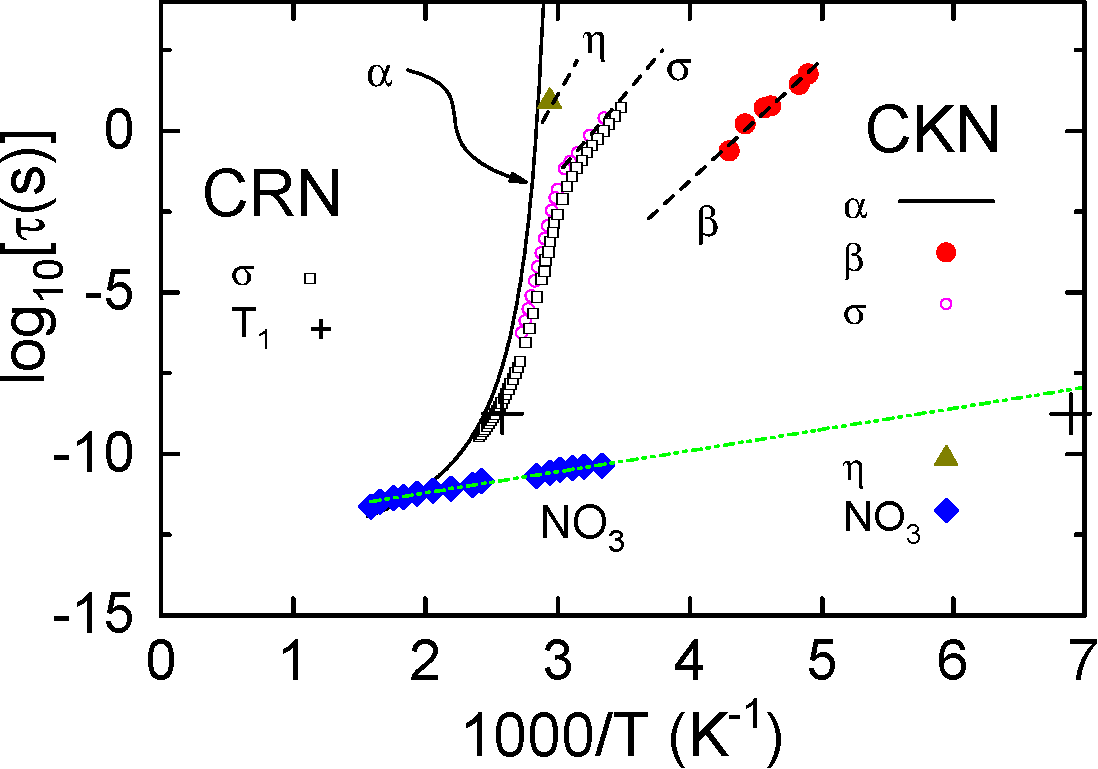
\includegraphics[width=.7\textwidth]{graphics/zuern/Plot1_b.pdf}
	\end{center}
	\caption{Relaxationskarte aus \cite{zuern_paper}, dargestellt in einem Arrhenius-Diagramm (logarithmierte Zeitkonstanten aufgetragen gegen die inverse Temperatur). Gezeigt sind ermittelte Zeitkonstanten aus Untersuchungen an CRN und CKN. Hierbei sind für diese Arbeit insbesondere der Betaprozess, dargestellt in rot, interessant. Die Daten hierzu stammen aus \cite{}} \label{fig:einl:zuernpaper}
\end{figure}

Eine Graph aus dem erwähnten Paper ist in Abbildung \ref{fig:einl:zuernpaper} zu sehen. Hier sind in CKN, kurz für Calciumkaliumnitrat, entdeckte Hinweise auf einen Betaprozess, dargestellt in rot, hervorzuheben. Die gestrichelte Linie durch die Punkte zeigt die lineare Fortsetzung der Punkte im Arrhenius-Diagramm an. Sollte dieser Trend standhalten, sollten bei Temperaturen in Bereichen kurz unter oder bei der Glasübergangstemperatur von $T_g = \SI{333}{K}$ Zeitkonstanten im hohen Mikrosekunden-Bereich zu erwarten sein. Zeitkonstanten dieser Größenordnungen lassen sich mit Methoden der NMR -- zum Beispiel der hier verwendeten Untersuchung von stimulierten Echos oder der Analyse von Linienformen von pulslängenabhängigen Spektren -- gut untersuchen.

Die Stoffe CKN und CRN ähneln sich sehr. Bis auf das gegen ein Rubidium-Atom ausgetauschte Kalium-Atom, welches der gleichen Hauptgruppe entstammt, teilen sie die gleiche Struktur, Glasübergangstemperatur und weitere Eigenschaften \cite{PIMENOV199793}. So ist beispielsweise auch in Abbildung \ref{fig:einl:zuernpaper} die Übereinstimmung von Leitfähigkeitsdaten $\sigma$ zwischen CRN und CKN zu erkennen. Daher ist es nachvollziehbar, für CRN und CKN ähnliche Zeitkonstanten eines Betaprozesses zu erwarten.

Während dieser Messungen wurde entdeckt, dass die Halbwertsbreite von CRN-Spektren zu höheren Temperaturen erst abnimmt -- was aufgrund der ansteigenden Bewegungsverschmälerung zu höheren Temperaturen zu erwarten ist -- aber bei Temperaturen ab $\SI{375}{K}$ wieder zunimmt. Dies widerspricht der naiven Erwartung, dass die Halbwertsbreite zu steigenden Temperaturen in diesem Fall lediglich abnehmen sollte. Um die Gründe dieses Phänomen zu klären wurden Spektren simuliert und ein Vergleich mit der Theorie der Quadrupol-Wechselwirkung zweiter Ordnung, welche hier entscheidende Einflüsse hat, durchgeführt.


Zunächst sollen in Kapitel \ref{chapter:theo} die theoretischen Grundlagen der NMR erläutert werden und eine Einführung in die Relaxation der Quadrupol-Wechselwirkung zweiter Ordnung gegeben werden. Kapitel \ref{chapter:simulation} beschreibt die für die Simulation verwendete Software mit zugehörigem Bewegungsmodell. Außerdem wird ein weiteres Bewegungsmodell vorgestellt, in der Zukunft facettiertere Untersuchungen ermöglichen könnte. In Kapitel \ref{chapter:exp_details} die verwendeten Apparaturen und Proben beschrieben, ehe in Kapitel \ref{chapter:experiment} die aufgenommenen Daten zunächst gezeigt, und dann ausgewertet und analysiert werden. Eine Zusammenfassung der Ergebnisse und ein Ausblick auf mögliche zukünftige Untersuchungen bilden den Abschluss der Arbeit.

\chapter{Theoretische Einführung}
\label{chapter:theo}

\section{Theoretische Grundlagen der NMR} \label{section:theo:grundlagen}


Ziel der NMR ist es, Kernspins einer Probe zu manipulieren und zu beobachten.
Da Spins $I$ über
\begin{align}
    \vec{\mu} = \gamma \hbar \vec{I}
\end{align}
mit magnetischen Dipolen $\mu$ verknüpft sind, ist die Beeinflussung von Spins mithilfe von Magnetfeldern möglich. Der Proportionalitätsfaktor $\gamma$ ist als gyromagnetisches Verhältnis bekannt und eine isotopenabhängige Konstante.

Werden die Kernspins einem Magnetfeld $\vec{B}_0 = (0, 0, B_{0,z})$ ausgesetzt, spalten die Energiezustände nach Zeeman auf. Die potentielle Energie eines magnetischen Dipols ist $E = - \vec{\mu} \vec{B}_0$. Mit obigen Beziehungen resultiert demnach $E = - \gamma \hbar I_z B_{0,z}$. Die Eigenwerte von $I_z$ lauten $m = -I, -I + 1, \dots, I - 1, I$; somit ist die Energiedifferenz zwischen zwei benachbarten Zuständen $\Delta E = E_{m+1} - E_{m} = - \gamma \hbar B_{0,z}$. Die damit verbundene Kreisfrequenz
\begin{align}
    \omega_L = \frac{\Delta E}{\hbar} = - \gamma B_{0,z} \label{eqn:lamorfrequenz}
\end{align}
ist die Larmorfrequenz oder Resonanzfrequenz. Der Konvention folgend wird $\omega_L$ nachfolgend als positiv angenommen.



In Anlehnung an das klassische Pendant, findet sich folgende Formel für den Drehimpuls $I$ und die Magnetisierung $M = \frac{1}{V} \sum_i \mu_i = \frac{\gamma \hbar}{V} \sum_i I_i$:
\begin{align}
    \frac{\text{d}\vec{M}}{\text{d}t} = \omega_L \times \vec{M}. \label{eqn:drehmoment}
\end{align}
Diese Gleichung lässt sich durch:
\begin{align}
    M_x (t) &= M_x(0) \cos(\omega_L t - \phi) \\
    M_y (t) &= M_y(0) \sin(\omega_L t - \phi) \\
    M_z (t) &= M_z(0).
\end{align}
lösen.

Dies bedeutet, dass aus der Gleichgewichtsorientierung $M_z$ ausgelenkte magnetische Dipole nicht zu dieser zurück relaxieren, sondern eine Ausweichbewegung vollziehen und mit der Kreisfrequenz $\omega = \omega_L$ um die Achse des Magnetfeldes präzedieren.

Um die folgenden Überlegungen einfacher zu gestalten, wird nun von dem Laborsystem in ein rotierendes Koordinatensystem übergegangen. Die Drehung des Koordinatensystems soll der der Magnetisierung dabei dergestalt gleichen, dass diese im neuen Koordinatensystem stationär erscheint; dies bedeutet also eine Drehung des Koordinatensystems um die Magnetfeldachse mit einer Kreisfrequenz $\omega_L$.

Dies hat nach Formel \eqref{eqn:lamorfrequenz} zur Folge, dass das Magnetfeld $B_0$ im rotierenden Koordinatensystem als geschwächt erscheint: $B_\text{eff} = B_0 - \frac{\omega}{\gamma}$. Ist $\omega = \omega_L$, so ist das effektive Magnetfeld null.


Neben diesem Vorwissen ist es nötig, Spins aktiv beeinflussen zu können, um in der Lage zu sein effektiv Informationen zu sammeln. Daher wird häufig die Probe in einer Spule untergebracht, deren Achse senkrecht zu der des Magnetfeldes steht; die Konvention richtet diese Spule entlang der x-Achse aus. Wird an der Spule eine Wechselspannung angelegt, werden die Spins einem entsprechenden Magnetfeld $\vec{B}_1 = 2 B_{1,x} \cos(\omega_1 t)$ ausgesetzt.

Da die Spule im Laborsystem stationär ist, rotiert das entstehende Magnetfeld im rotierenden Koordinatensystem mit $-\omega$. Um dies zu vermeiden wird $B_1$ als Superposition zweier Drehungen dargestellt:
\begin{align}
    \vec{B}_1 = B_1 \left[ \myvec{\cos(\omega) \\ \sin(\omega) \\ 0} + 
                      \myvec{\cos(\omega) \\ -\sin(\omega) \\ 0} \right].
\end{align}
Im rotierenden Koordinatensystem ergibt sich dies nun zu
\begin{align}
    \vec{B}_1 = B_1 \left[ \myvec{1 \\ 0 \\ 0} + 
                      \myvec{\cos(2\omega) \\ -\sin(2\omega) \\ 0} \right],
\end{align}
was bedeutet, dass sich das Magnetfeld als eine Superposition aus einem stationären Teil und einem Teil, der mit $-2\omega$ rotiert, darstellen lässt. Letzter kann aufgrund der hohen Frequenz vernachlässigt werden -- dies ist als „rotating wave approximation“ bekannt --, sodass nur der stationäre Anteil im rotierenden Koordinatensystem verbleibt.

Wird das $B_1$-Feld vom Experimentierenden aktiviert, so vollführt die mittlere Magnetisierung nach Formel \eqref{eqn:drehmoment} eine Präzessionsbewegung senkrecht zu diesem Magnetfeld. Mit einem Puls einer bestimmten Länge lassen sich die Magnetisierung so beispielsweise mit einem 90$^\circ$-Puls in die x-y-Ebene klappen oder mit einem 180$^\circ$-Puls invertieren. Durch das Kombinieren von Pulsen lassen sich Pulsfolgen entwickeln, um interessante Eigenschaften einer Probe zu untersuchen.

In allen realen Systemen gibt es durch unterschiedliche Wechselwirkungen Relaxationen der longitudinalen und transversalen Magnetisierung, welche im nächsten Kapitel behandelt werden sollen.



\section{Theoretische Aspekte der Relaxation} \label{section:theo:relax}

Werden Kernspins, beispielsweise durch einen 90$^\circ$-Puls, aus ihrem Gleichgewichtszustand ausgelenkt, sind sie nicht mehr im Boltzmann-Gleichgewicht und sollten daher in den Gleichgewichtszustand relaxieren. Bei den für die hier verwendeten Temperaturen von mehreren Hundert Kelvin sind jedoch die Besetzungsverhältnisse $\frac{N_+}{N_-} = \exp (\frac{- \hbar \gamma B}{k_B T})$ fast beliebig nah an 1 und die thermisch induzierten Relaxationsraten daher nahezu verschwindend gering. Energie aus anderen Quellen kann jedoch Übergänge zwischen den Zuständen und damit Relaxation ermöglichen.

Durch die zufälligen Bewegungen der Atome oder Moleküle einer Probe ändern sich für ein untersuchtes Atom die entsprechenden lokalen elektromagnetischen Felder. Enthält das Spektrum der Feldfluktuationen Frequenzen der Larmorfrequenz (oder, je nach Wechselwirkung, Vielfache davon), können Relaxationsprozesse auftreten und somit schlussendlich die gesamte Magnetisierung in den Gleichgewichtszustand zurückkehren. Es ist offensichtlich, dass die Spektraldichte $J(\omega)$, die die Häufigkeit der entsprechenden Frequenzen angibt, eine wichtige Rolle bei der Beschreibung der Relaxation spielt. Zu berücksichtigende Wechselwirkungen sind -- je nach untersuchtem Stoff bzw. Kern -- zum Beispiel die chemische Verschiebung, die Dipol-Dipol-Wechselwirkung oder die Quadrupol-Wechselwirkung.

Die durch die Bewegung der Atome induzierte Relaxation wird longitudinale Relaxation oder Spin-Gitter-Relaxation genannt; die zugehörige Konstante $T_1$ gibt an, auf welcher Zeitskala sie stattfindet.

Die transversale Relaxation oder Spin-Spin-Relaxation basiert, wie der Name suggeriert, auf Wechselwirkungen zwischen mehreren Spins. Die Stärke der Dipol-Dipol-Wechselwirkung ist für jeden Spin aufgrund der leicht verschiedenen Positionen und Winkeln der Spins zueinander ebenfalls leicht unterschiedlich sowie winkelabhängig. Das bedeutet, dass nicht alle Spins mit der gleichen Frequenz prädizieren, sondern sich mit der Zeit eine Phase bildet und somit die mittlere Magnetisierung reduziert wird. Die Größe dieser Relaxation wird durch $T_2$ beschrieben.


Während sich die Grundlagen des letzten Kapitels gut und verständlich mit klassischen Konzepten darstellen lassen, ist es für die theoretische Beschreibung der Relaxation unabdinglich, zu quantenmechanischen Rechnungen überzugehen. Die folgenden Rechnungen finden sich in detaillierterer Form in \cite[S. 191-195]{benesi} und \cite[S. 108-110]{spiess}.

Der Ausgangspunkt ist der Dichteoperator $\hat{\rho}(t)$, der interne Hamilton-Operator im rotierenden Koordinatensystem $\hat{H}_\text{rot}(t)$, und die Liouville-von-Neumann Gleichung
\begin{align}
    \frac{\text{d} \hat{\rho}_\text{rot}}{\text{d}t} = -i [\hat{H}_\text{rot}(t), \hat{\rho}_\text{rot}].
\end{align}

$\hat{H}_\text{rot}(t)$ ist aufgrund der erwähnten zufälligen Molekülbewegungen nicht konstant, weswegen die Gleichung bis zur zweiten Ordnung integriert werden muss. Wird davon die zeitliche Ableitung gebildet, ergibt sich mit der Substitution $t' = t - \tau$ folgende Gleichung:
\begin{align}
    \frac{\text{d} \hat{\rho}_\text{rot}}{\text{d}t} = - i [\hat{H}_\text{rot}(t), \hat{\rho}_\text{rot}(0)] - \int_0^t \text{d} \tau \left[\hat{H}_\text{rot}(t), [\hat{H}_\text{rot}(t-\tau), \hat{\rho}_\text{rot}(0)] \right].
\end{align}

Nach \cite[S. 276]{spiess} sind vier Annahmen notwendig, um schlussendlich zur Mastergleichung zu gelangen:
\begin{itemize}
\item $\hat{H}_\text{rot}(t)$ und $\hat{\rho}_\text{rot}(0)$ sind unkorreliert.
\item $\hat{\rho}_\text{rot}(0)$ kann durch $\hat{\rho}_\text{rot}(t)$ ersetzt werden.
\item Die Integration kann von $t$ auf $\infty$ ausgeweitet werden.
\item Höhere als die zweite Ordnung der vorherigen Gleichung können vernachlässigt werden.
\end{itemize}
Zudem soll $\hat{\rho}' = \hat{\rho}_\text{rot} - \hat{\rho}_\text{eq}$ gelten, sodass $\hat{\rho}'$ die Abweichungen vom Gleichgewichtszustand $\hat{\rho}_\text{eq}$ darstellt.
Damit ergibt sich:
\begin{align}
    \frac{\text{d} \hat{\rho}'}{\text{d}t} = - \int_0^t \text{d} \tau \left< \left[\hat{H}_\text{rot}(t), [\hat{H}_\text{rot}(t-\tau), \hat{\rho}'(t)] \right] \right>. \label{eqn:mastergleichung}
\end{align}

Das Lösen dieser Gleichung gestaltet sich recht umfangreich, daher soll die Rechnung hier nur in den groben Zügen nachvollzogen werden.
Für die Darstellung des Hamilton-Operators werden sphärische Tensoren $\hat{T}^{l,m}$ verwendet, sodass sich mit den Laborsystem-Tensoren $A^{l,m}(t)$, eingesetzt in die Mastergleichung \eqref{eqn:mastergleichung}, Folgendes ergibt:
\begin{align}
\begin{split}
    \frac{\text{d} \hat{\rho}'}{\text{d}t} =& -\sum_{l_1 = 0}^2 \sum_{l_2 = 0}^2 \sum_{m_1 = -l}^l \sum_{m_2 = -l}^l (-1)^{m_1+m_2} e^{i(m_1+m_2) \omega_0 t} \left[\hat{T}_{l_1,m_1}, [\hat{T}_{l_2,m_2}, \hat{\rho}'(0)] \right] \\ &\times \int_0^\infty \left< A_{l_1,m_1}(t) A_{l_2,m_2}(t-\tau) \right> e^{i m_2 \omega_0 \tau} \text{d} \tau
\end{split}
\end{align}

Da der Hamiltonoperator der Wechselwirkung $\hat{H}_\text{rot}(t)$ klein ist (gegenüber der Zeeman-Wechselwirkung), ist auch $\frac{\text{d} \hat{\rho}'}{\text{d}t}$ klein. Durch diese langsame Änderung mit der Zeit mitteln sich bei dem schnell variierenden $e^{i(m_1+m_2) \omega_0 t}$ alle Elemente außer bei $m_1 = - m_2$ heraus. Gleichzeitig muss, wegen der Wigner-Orthogonalität der Operatoren, $l_1 = l_2$ gelten.

Es ergibt sich eine Autokorrelationsfunktion von $A$; das Integral über diese kann nach einigen Umformungen als Spektraldichte $J(\omega)$ identifiziert werden. Schlussendlich kann damit die Mastergleichung wie folgt formuliert werden:
\begin{align}
    \frac{\text{d} \hat{\rho}'}{\text{d}t} = - C_\gamma \sum_{l = 0}^2 \sum_{m = -l}^l (-1)^{m+l} \left[\hat{T}_{l,m}, [\hat{T}_{l,-m}, \hat{\rho}'(0)] \right] \times J_{l,m}(m \omega_0).
\end{align}
$C_\gamma$ ist dabei eine vom Hamiltonoperator abhängige Konstante.

Wird diese Gleichung unter Ausnutzung von Kommutatorrelationen gelöst, ergeben sich folgende Gleichungen, die zur longitudinalen bzw. transversalen Relaxation korrespondieren:
\begin{align}
    \Braket{\frac{\text{d} \hat{I}_z}{\text{d}t}} =& - C_\gamma \sum_{l = 0}^2 \sum_{m = -l}^l (-1)^{l+m} \left[\hat{T}_{l,m}, \hat{T}_{l,-m}\right] \times m J_{l,m}(m \omega_0) \label{eqn:long_relax_theorie} \\
    \Braket{\frac{\text{d} \hat{I}_\pm}{\text{d}t}} =& - C_\gamma \sum_{l = 0}^2 \sum_{m = -l}^l (-1)^{l+m} \left[\hat{T}_{l,m \pm 1}, \hat{T}_{l,-m}\right] \times \sqrt{l(l+1) - m(m \pm 1)} \times m J_{l,m}(m \omega_0) \label{eqn:trans_relax_theorie}
\end{align}


% \begin{align}
% \begin{split}
%     \Braket{\frac{\text{d} \hat{I}_z}{\text{d}t}} =& -\sqrt{2} C_\gamma \left( J(-\omega) + J(\omega) \right) \Braket{\hat{I}^{1,0}} \\
%     & - \sqrt{\frac{2}{5}} C_\gamma \left( 4J(-2\omega) + 4J(2\omega) + J(-\omega) + J(\omega) \right) \Braket{\hat{I}^{1,0}} \\
%     & - \sqrt{\frac{2}{5}} C_\gamma \left( 2J(-2\omega) + 2J(2\omega) - 2J(-\omega) - 2J(\omega) \right) \Braket{\hat{I}^{3,0}} \label{eqn:long_relax}
% \end{split}
% \end{align}
% \begin{align}
% \begin{split}
%     \Braket{\frac{\text{d} \hat{I}^{\pm}}{\text{d}t}} =& -C_\gamma (2J(0) + 2J(\mp \omega)) \Braket{\hat{I}^{1,\pm 1}} \\
%     & - \sqrt{\frac{2}{5}} C_\gamma (2J(\mp 2\omega) + 3J(\mp \omega) + 3J(0) + 2J(\pm \omega)) \Braket{\hat{I}^{1,\pm 1}} \\
%     & - \sqrt{\frac{2}{5}} C_\gamma (\sqrt{6}J(\mp 2\omega) - \sqrt{6}J(\mp \omega) - \sqrt{6}J(0) + \sqrt{6}J(\pm \omega)) \Braket{\hat{I}^{3,\pm 1}} \label{eqn:trans_relax}
% \end{split}
% \end{align}
Verschiedene Wechselwirkungs-Hamiltonoperatoren haben unterschiedliche Lösungen für die Kommutatorrelationen in Gleichungen \eqref{eqn:long_relax_theorie} und \eqref{eqn:trans_relax_theorie}, weswegen sich für Wechselwirkungen spezifische Relaxationen ergeben.




\section{Quadrupol-Relaxation und Spektraldichten} \label{section:theo:eckert}

Häufig mit der NMR aufgenommene Daten umfassen $T_1$- und $T_2$-Messungen, sowie Spektren, wobei deren Schwerpunkte oder Breiten interessante Kenngrößen sein können. All diese Eigenschaften sind in der Regel nuklid- und temperaturabhängig. So bewirkt beispielsweise die bei höherer Temperatur größere Bewegung der Atome oder Moleküle ein Herausmitteln der Effekte, die sonst zu einer Verbreiterung des Spektrums führen würden und es tritt Bewegungsverschmälerung oder „motional narrowing“ auf. Ein Abweichen von diesem Verhalten in den beobachteten Daten (siehe Abbildung \ref{fig:triple_vergleich}, Mitte) führte zu dem Versuch, das Phänomen mit den im Folgenden aufgeführten theoretischen Erläuterungen zu erklären. Aus diesem Grund erstreckt sich die Untersuchung nur auf den relevanten Temperaturbereich von $\SI{350}{K}$ bis $\SI{500}{K}$.

Für $^{87}$Rb-NMR ist die Quadrupol-Wechselwirkung und damit auch die zugehörige Relaxation von besonderem Interesse. Es wird angenommen, dass ein sich im thermischen Gleichgewicht befindendes Spinsystem mit einem 90$^\circ$-Puls aus diesem ausgelenkt wird.

Für die longitudinale Relaxation sagt die Theorie nach \cite{hubbard} im non-extreme narrowing Bereich, also bei $\omega \tau_c \gg 1$, eine biexponentielle Relaxation vorher:
\begin{align}
    - \frac{\Braket{I_z} - \Braket{I_z(\infty)}}{2\Braket{I_z(\infty)}} = \frac{4}{5}e^{-t/T_{1a}} + \frac{1}{5}e^{-t/T_{1b}}.
\end{align}
Dabei sind $T_{1a}$ und $T_{1b}$ gegeben als
\begin{align}
    1/T_{1a} &= 2J(2\omega_0) \\
    1/T_{1b} &= 2J(\omega_0).
\end{align}
Im extreme narrowing limit, $\omega \tau_c \ll 1$, verschmelzen die Exponentialfunktionen zu einer, da dort $J(2\omega_0) \approx J(\omega_0)$. Eine Spektraldichte $J \sim \tau_c / (1 + \omega^2 {\tau_c}^2)$ vereinfacht sich im Fall $\omega \tau_c \ll 1$ zu $J \sim \tau_c$, wodurch die Frequenzabhängigkeit verschwindet.

In der Praxis unterstützen die Daten laut \cite{eckert} allerdings auch sonst eine biexponentielle Relaxation selten, stattdessen ist eine monoexponentielle Funktion wie aus der bekannten BPP-Theorie \cite{bpp} eine hinreichende Näherung. Dort ergibt sich
\begin{align}
    1/T_1 &= K (J(\omega_0) + 4J(2\omega_0)) \label{eqn:bpp}
\end{align}
als einziger $T_1$-Wert, mit der kernabhängigen Konstante $K$.

Die Spektraldichte $J(\omega)$ kann je nach Modell unterschiedlich sein. In diesem Kontext wird eine Spektraldichte verwendet, die auf einer einzelnen Korrelationszeit $\tau_c$ für die Beschreibung der Molekülbewegungen basiert \cite{eckert}:
\begin{align}
    J(\omega) &= \frac{\pi^2}{5} {C_Q}^2 \left( 1 + \frac{\eta^2}{3} \right) \frac{\tau_c}{1 + \omega^2 {\tau_c}^2}. \label{eqn:spektraldichte_j}
\end{align}
Dabei ist $C_Q$ die Kopplungskonstante der Quadrupol-Wechselwirkung und $\eta$ der Asymmetrieparameter der Beschreibung des elektrischen Feldgradienten. Für $\tau_c$ wird oft ein Arrhenius-Gesetz mit der Aktivierungsenergie $E_a$ und dem präexponentiellen Faktor $\tau_{co}$ angenommen:
\begin{align}
    \tau_c = \tau_{co} \exp \left( \frac{E_a}{k_B T} \right).
\end{align}


Für die transversale Relaxation -- wieder nach einem 90$^\circ$-Puls -- gibt die Theorie \cite{werbelow}
\begin{align}
    \frac{\Braket{I_x} + \Braket{I_y}}{i\Braket{I_z}} = \frac{2}{5}e^{-i(\omega_0 + \omega_c^{(2)})t}e^{-t/T_{2c}} + \frac{3}{5}e^{-i(\omega_0 + \omega_s^{(2)})t}e^{-t/T_{2s}}. \label{eqn:trans_relax}
\end{align}
Auch hier sind zwei Exponentialfunktionen vorhanden (deren Effekt auch in Daten beobachtet werden kann); sie lassen sich als zugehörig zum Zentralübergang (Index $c$) bzw. zu den Satellitenübergängen (Index $s$) identifizieren. Dies kann, nach \cite{werbelow}, auch das Intensitätsverhältnis $\frac{2}{5}:\frac{3}{5}$ zwischen Zentralübergang und Satellitenübergängen wie folgt erklären: Die longitudinale Magnetisierung $\Braket{I_z}$ lässt sich durch die Populationen $P_i$ der jeweiligen Zustände $i$ ausdrücken als $\Braket{I_z} = (3/2)P_{3/2} + (1/2)P_{1/2} - (1/2)P_{-1/2} - (3/2)P_{-3/2}$. Einfaches Umformen ergibt $\Braket{I_z} = (3/2)(P_{3/2} - P_{1/2}) + (4/2)(P_{1/2} - P_{-1/2}) + (3/2)(P_{-1/2} - P_{-3/2})$. Hier lassen sich erster und dritter Term den Satellitenübergängen zuordnen, der zweite dem Zentralübergang; in der Summe ergibt sich dann genau das Verhältnis $\frac{4}{2}:\frac{6}{2}$ oder $\frac{2}{5}:\frac{3}{5}$.

$\omega_{c/s}$ sind die Schwerpunkte des Spektrums, die sich neben der Breite aus der transversalen Relaxation gewinnen lassen. Diese sind mit dem Imaginärteil der Spektraldichte, dem dynamischen Frequenzverschiebung zweiter Ordnung, $Q(\omega, \tau_c)$, verbunden \cite{eckert}:
\begin{align}
    \omega_c^{(2)} &= Q(2\omega_0) - Q(\omega_0) \\ \label{eqn:schwerpunkt}
    \omega_s^{(2)} &= Q(\omega_0), \\
    \text{wobei } Q(\omega) &= \frac{\pi^2}{5} {C_Q}^2 \left( 1 + \frac{\eta^2}{3} \right) \frac{\omega {\tau_c}^2}{1 + \omega^2 {\tau_c}^2}.
\end{align}

Für die entsprechenden $T_2$-Werte $T_{2c}$ und $T_{2s}$ ergeben sich folgende Zusammenhänge \cite{eckert}:
\begin{align}
    1/T_{2c} &= J(\omega_0) + J(2\omega_0) \\
    1/T_{2s} &= J(0) + J(\omega_0).
\end{align}

Wird für eine solche Messung ein FID (free induction decay) aufgenommen, so lässt dieser sich mittels einer Fouriertransformation in ein Frequenzspektrum überführen. Bei der hier relevanten Exponentialfunktion entsteht eine Lorentzfunktion, deren Breite oder FWHM (full width at half maximum) $\Delta_{c/s}$ wie folgt mit $T_{2c}$ bzw. $T_{2s}$ verknüpft ist \cite{werbelow}:
\begin{align}
    \Delta_c &= 1/(\pi T_{2c}) \\ \label{eqn:fwhm}
    \Delta_s &= 1/(\pi T_{2s}).
\end{align}

Neben der hier vorgestellten Spektraldichte $J(\omega)$, die von einer einzelnen Korrelationszeit $\tau_c$ zur Beschreibung der Molekülbewegung ausgeht, existieren noch weitere Modelle, denen verschiedene Verteilungen von $\tau_c$ zugrunde liegen. Bekannte Spektraldichten sind von Cole-Cole ($J_{CC}$) und von Cole-Davidson ($J_{CD}$) \cite[S. 105-108]{beckmann_relaxation}, angepasst mit dem entsprechenden Vorfaktor aus Formel \eqref{eqn:spektraldichte_j}:
\begin{align}
    J_{CC}(\omega, \tau_c, \alpha) &= \frac{\pi^2}{5} {C_Q}^2 \left( 1 + \frac{\eta^2}{3} \right) \frac{2}{\omega} \sin \left( \frac{\alpha \pi}{2} \right) \left[ \frac{(\omega \tau_c)^\alpha}{1 + (\omega \tau_c)^{2\alpha} + 2 (\omega \tau_c)^\alpha \cos (\alpha \pi / 2)} \right], \\
    J_{CD}(\omega, \tau_c, \gamma) &= \frac{\pi^2}{5} {C_Q}^2 \left( 1 + \frac{\eta^2}{3} \right) \frac{2}{\omega} \left\{ \frac{\sin [\gamma \arctan(\omega \tau_c)]}{(1 + \omega^2 {\tau_c}^2)^{2\gamma}} \right\}
\end{align}
Für $\alpha = 1$ bzw. $\gamma = 1$ korrespondieren diese Spektraldichten zu BPP.





\section{Theoretische Beschreibung experimenteller CRN-Daten} \label{section:theo:daten}


Es wurde untersucht, ob vorliegende gemessenen Daten mit den beschriebenen Theorien in Einklang gebracht werden können. Dafür wurden die Daten zu $T_1$, zu Spektren untersucht; die $T_1$-Daten stammen dabei aus Messungen von C. Zürn \cite{zuern_paper} an einer 2Ca(NO$_3$)$_2$-3RbNO$_3$-Probe, während alle weiteren Daten mit der von Zürn verwendeten Probe im Rahmen dieser Masterarbeit aufgenommen wurden.

Um eine Übereinstimmung zur Theorie feststellen zu können, müssen sich alle Datensätze mit dem gleichen Satz geteilter Parameter beschreiben lassen. Im Falle der Spektraldichte $J(\omega)$ sind dies $C_Q$ und $\tau_{co}$; für $J_{CC}$ und $J_{CD}$ sind $\alpha$ bzw. $\gamma$ zusätzliche Parameter.

Nach \cite{PIMENOV199793} wird für CRN für die Korrelationszeit ein Vogel-Fulcher-Gesetz
\begin{align}
    \tau_c = \tau_{co} \exp \left( \frac{D T_\text{VF}}{T-T_\text{VF}} \right)
\end{align}
mit dem strength index $D = \SI{3.5}{}$, der Vogel-Fulcher-Temperatur $T_\text{VF} = \SI{294}{K}$ und dem Frequenzfaktor $\tau_{co} = \SI{5.1e-14}{s}$ (der beim Vergleich mit den Daten dennoch als freier Parameter angesehen werden soll um dem Fit eine größtmögliche Flexibilität zu erlauben) angenommen.

\begin{wrapfigure}{r}{0.5\textwidth}
  \vspace{-20pt}
  \begin{center}
    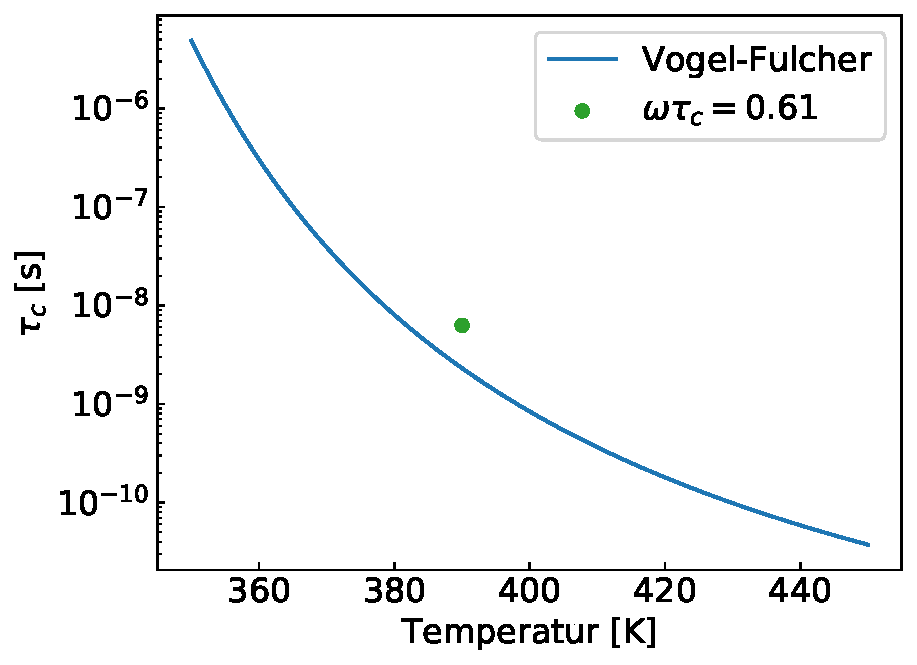
\includegraphics[width=0.49\textwidth]{graphics/zwischenbericht/tau_c_arrhenius_vogel_fulcher.pdf}
  \end{center}
  \vspace{-20pt}
  \caption{Vergleich von Korrelationszeiten basierend auf Vogel-Fulcher-Gesetz \label{fig:korrelationszeiten}}
\end{wrapfigure}
Am $T_1$-Minimum nach Gleichung \eqref{eqn:bpp} gilt $\omega \tau_c \approx \SI{0.61}{}$ \cite[S. 629]{omegatau061}. Das $T_1$-Minimum kann in den Daten bei etwa $T_\text{min} = \SI{390}{K}$ gefunden werden; die Larmorfrequenz liegt bei $\omega_L = \SI{97.1722}{MHz}$, was bedeutet, dass bei $T_\text{min}$ gilt $\tau_c \approx \frac{\SI{0.61}{}}{\omega_L} \approx \SI{6.28}{\nano s}$. Vergleicht man das Vogel-Fulcher-Gesetz mit diesem Punkt, lässt sich erkennen, dass eine gute Übereinstimmung vorliegt.


Die aufgenommenen Daten unterstützen eine biexponentielle Interpretation wie in \eqref{eqn:trans_relax} nur schwerlich, daher wurde lediglich der deutlich zu beobachtende Anteil des Zentralübergangs, $\Delta_c$ und $\omega_c^{(2)}$, für die entsprechenden FWHM- bzw. Schwerpunkts-Daten betrachtet. Für die $T_1$-Daten wird Formel \eqref{eqn:bpp} verwendet. Um einen Ausgangspunkt für die Analyse zu schaffen, wurden alle Fits per Hand erstellt, wobei durch das Ändern der Parameter versucht wurde eine möglichst gute Übereinstimmung zu erreichen.

Für die Spektraldichte $J(\omega)$ kann, wie in Abbildung \ref{fig:triple_vergleich} zu sehen, mit $\eta^2 = 42 - 24 \sqrt{3} \approx \SI{0.43}{}$ \cite{caer} und den Parametern $C_Q = \SI{3e6}{Hz}$ und $\tau_c = \SI{3.9e-14}{s}$ eine vergleichsweise gute Übereinstimmung für die $T_1$-Werte erreicht werden, die Flanken unterscheiden sich jedoch deutlich. Die Abweichungen der FWHM-Werten und der Schwerpunkte sind mit einem Faktor von etwa 4 bzw. etwa 2 bedeutend.
\begin{figure}[htbp]
    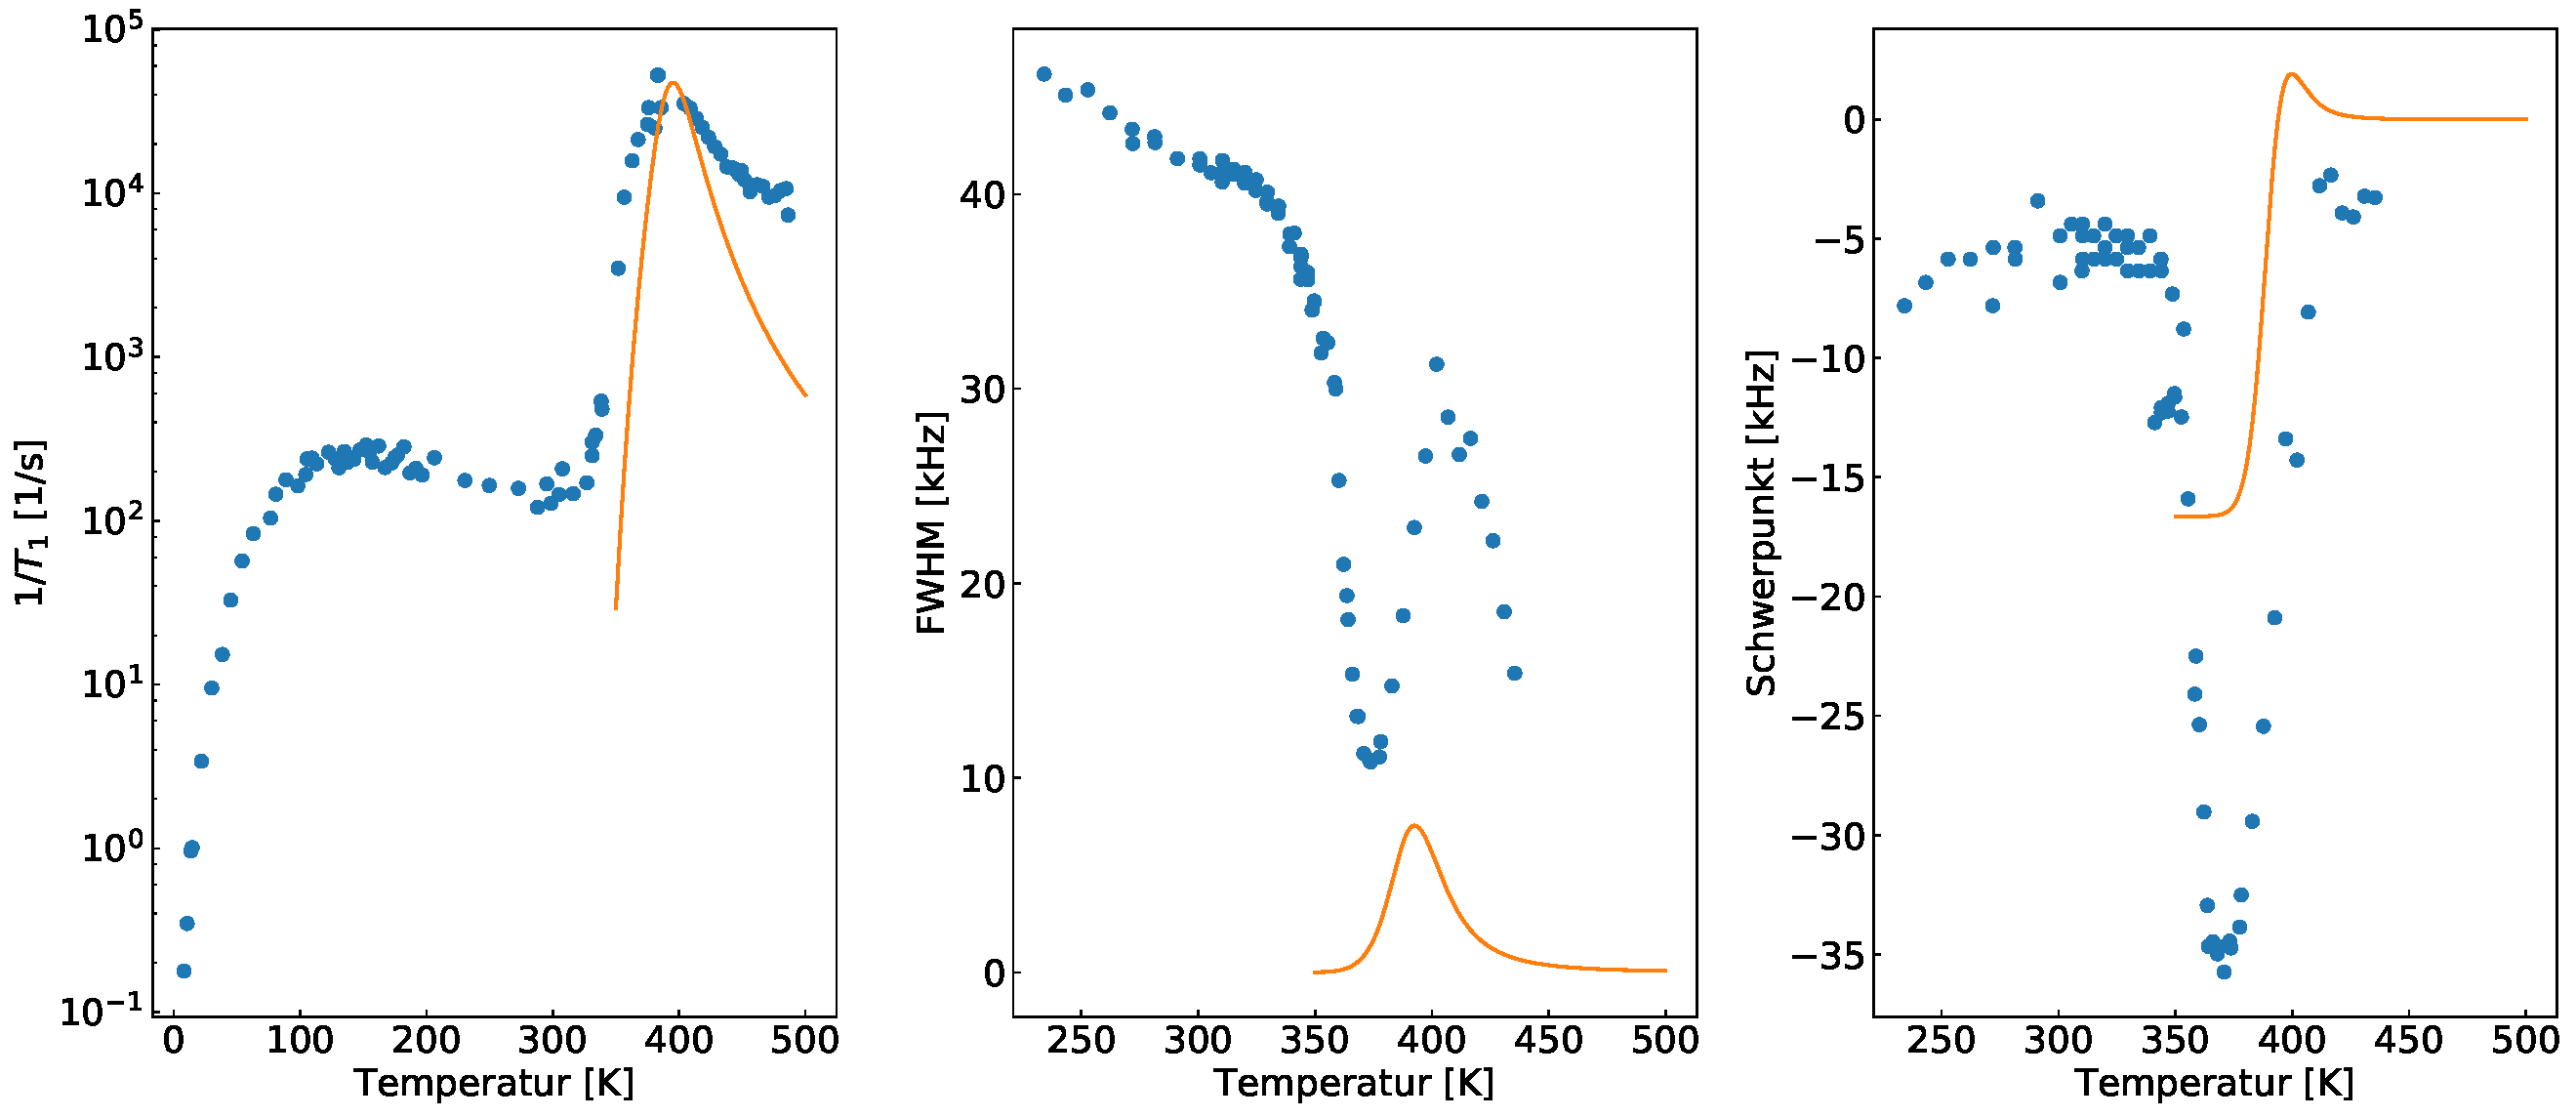
\includegraphics[width=\textwidth]{graphics/zwischenbericht/J_fertig.pdf}
    \caption{Vergleich der $T_1$-, FWHM- und Schwerpunkts-Daten (in blau) und der angepassten Theoriekurven (in orange). \label{fig:triple_vergleich}}
\end{figure}

Eine mögliche Erklärung für die Abweichung der FWHM-Werte könnte sein, dass in diesem Fall nicht, wie nach Formel \eqref{eqn:fwhm}, nur $T_2$, sondern auch das bei Temperaturen um $\SI{400}{K}$ mit etwa $\SI{50}{\micro s}$ äußerst kurze $T_1$ zur Verbreiterung des Spektrums und damit zu dessen FWHM-Werten beiträgt. Erste Versuche, den Effekt der $T_1$-Relaxation aus dem Spektrum herauszurechnen, scheinen vielversprechend. Für die Abweichungen der Schwerpunkts-Daten von der Theorie steht eine entsprechende Erklärung noch aus.

Aus diesem Grund jedoch soll für die Spektraldichten $J_{CC}$ und $J_{CD}$ die FWHM-Werte zunächst nicht betrachtet werden. Gleiches gilt für den Schwerpunkt, da die entsprechenden Imaginärteile der Spektraldichten, $Q_{CC}$ und $Q_{CD}$, nicht zur Verfügung stehen.

Für die Parameter $C_Q = \SI{2.85e6}{Hz}$, $\tau_c = \SI{7e-15}{s}$ und $\alpha = \SI{0.38}{}$ kann mit der Spektraldichte $J_{CC}$ in diesem Temperaturbereich eine noch bessere Übereinstimmung zu den $T_1$-Daten erzielt werden, für die Parameter $C_Q = \SI{2.7e6}{Hz}$, $\tau_c = \SI{4.4e-14}{s}$ und $\gamma = \SI{0.66}{}$ erreicht die Spektraldichte $J_{CD}$ eine leicht bessere Übereinstimmung als die Spektraldichte $J$; die entsprechenden Plots sind in Abbildung \ref{fig:j_cc_j_cd} zu finden.
% \begin{figure}[htbp]
%     \subfigure{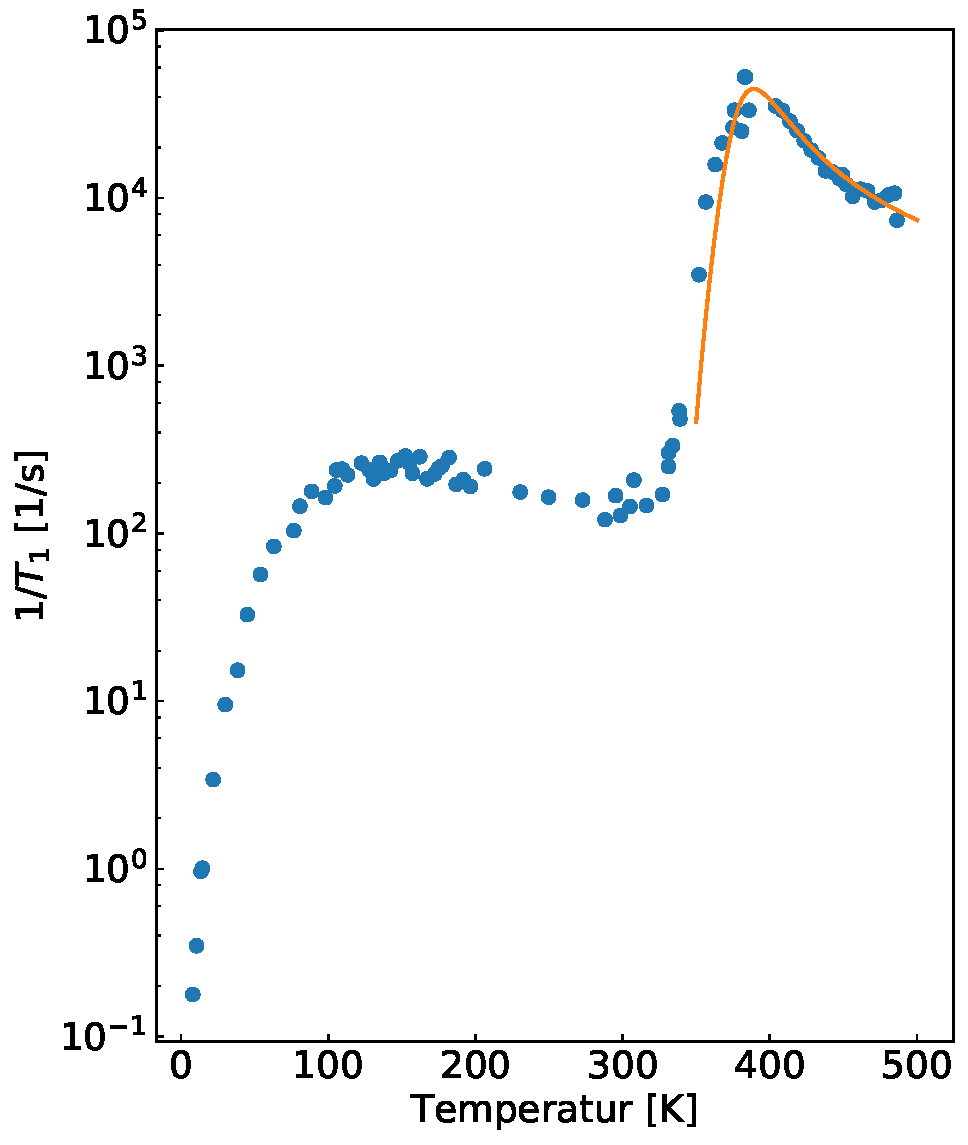
\includegraphics[width=0.49\textwidth]{graphics/zwischenbericht/J_cc.pdf}}\hfill
%     \subfigure{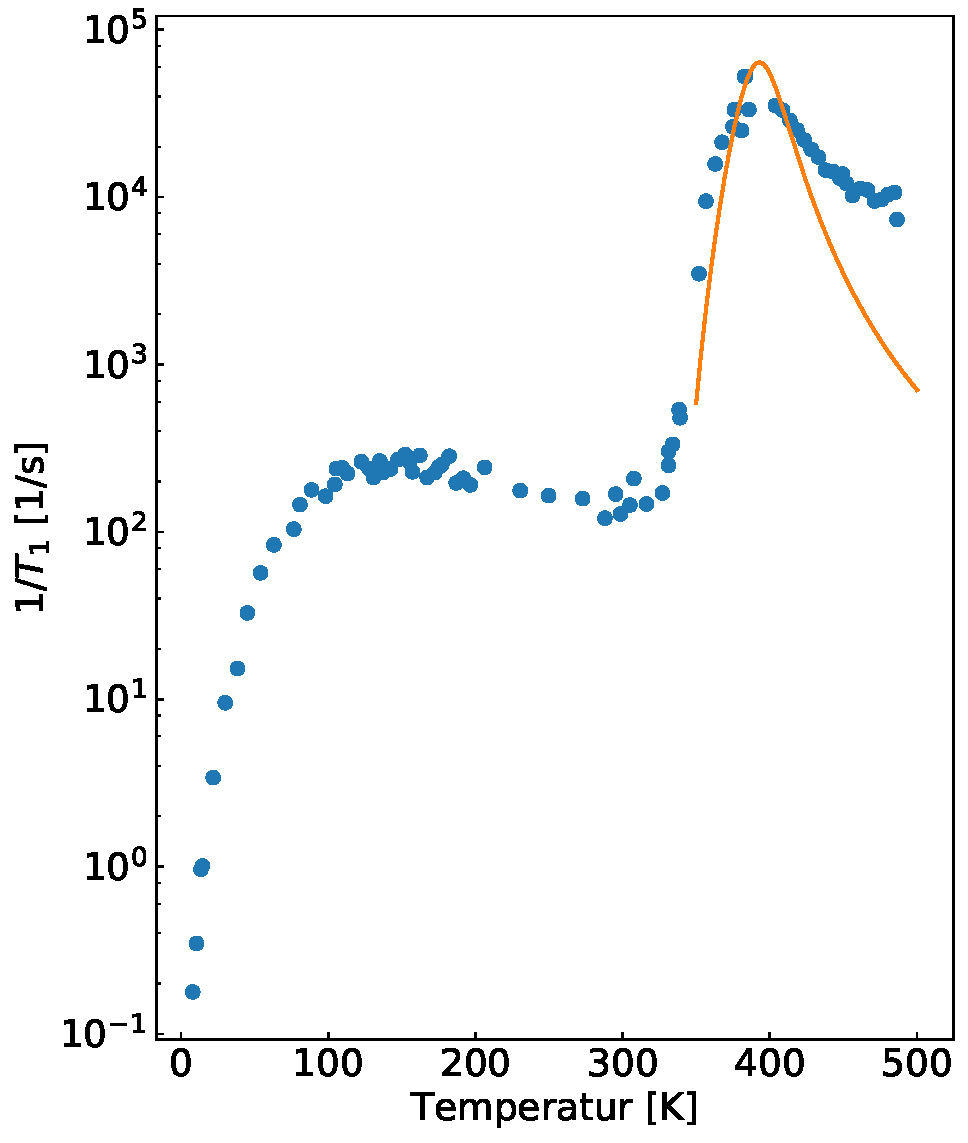
\includegraphics[width=0.49\textwidth]{graphics/zwischenbericht/J_cd.pdf}}
%     \caption{Spektraldichten $J_{CC}$ (links) und $J_{CD}$ (rechts), angepasst an die Daten \label{fig:j_cc_j_cd}}
% \end{figure}
Die nächsten Schritte in dieser Untersuchung sollen darin bestehen, die Auswirkungen der $T_1$-Relaxation auf die Spektrums-Breite zu bestimmen und schlussendlich zu ergründen, ob sich die Messdaten sich mit diesen Theorien zufriedenstellend erklären lassen.





\section{Echos} \label{section:theo:echos}

Um Größen wie $T_1$ und $T_2$ zu messen, werden unterschiedliche Pulsfolgen, also Sequenzen von RF-Pulsen mit bestimmten Längen und Abständen zwischeneinander, ausgenutzt.

Um die longitudinale Relaxation $T_1$ zu messen, wurde folgende Pulsfolge verwendet:
*** Bild
Der erste Puls, ein $\SI{180}{\degree}$-Puls, invertiert die Magnetisierung von $M_\infty$ zu $M_{-\infty}$, wonach diese anfängt zu relaxieren. Da die longitudinale Magnetisierung aufgrund der Spulengeometrie nicht detektierbar ist, muss sie mit $\SI{90}{\degree}$-Puls in die Detektionsebene geklappt werden. Wird dies nach der Evolutionszeit $t_p$ getan, kann also die relaxierende Magnetisierung in Abhängigkeit von $t_p$ bestimmt werden. Der letzte Puls, ein $\SI{180}{\degree}$-Puls, wird Hahn-Echo genannt. Häufig liegen die Momente direkt nach einem Puls in der Totzeit des Detektors, sodass die Magnetisierung faktisch erst gemessen werden kann, wenn sie eine gewisse Zeit abgeklungen ist. Um dieses Problem zu umgehen wird das Hahn-Echo verwendet. 




Nach einer Zeit $\tau_x$ *** nach dem letzten Puls einer Pulsfolge wird die Magnetisierung mit einem $\SI{180}{\degree}$-Puls umgeklappt. Die angesammelten Phasen werden in gleicher Weise subtrahiert, sodass nach der Zeit $2 \tau_x$ *** ein Echo mit maximaler Magnetisierung zu detektieren ist. Das Hahn-Echo kann Teile der Magnetisierung refokussieren, die linear in $I_z$ sind. Dazu zählen zum Beispiel *** und lokale Feldinhomogenitäten. Nicht jedoch wiedergewonnen werden können Teile der Magnetisierung, die durch *** -> T2 verloren wurden. Damit dieser Einfluss bei den Messungen konstant ist, wird in diesem Fall das gleiche $\tau_x$ *** für alle Messungen verwendet.

Es lässt sich so aber offensichtlich mit folgender Pulsfolge $T_2$ bestimmen: Ein $\SI{90}{\degree}$-Puls kippt die Magnetisierung aus dem Gleichgewicht in die Detektionsebene, wo sie sodann anfängt zu dephasieren. Nach der Zeit $\tau_x$ *** wird ein Hahn-Echo durchgeführt und nach $2 \tau_x$ kann die verbliebene Stärke der Magnetisierung gemessen werden. $T_2$ kann so in Abhängigkeit von $\tau_x$ *** aufgenommen werden.

Sowohl an $T_1$- als auch an $T_2$-Daten können Varianten einer Kohlrauschfunktion gefittet werden
*** Formeln
Dabei handelt es sich um Exponentialfunktionen, die mit einem Exponenten $\beta$ gestrecjt werden können. Dieser Exponent erlaubt Abweichungen von der BPP-Theorie, die vin einer einzelnen Korrelationszeit $\tau_c$ ausgeht. ***

% \chapter{Bewegungsmodelle}\label{sec:theo:bewegungsmodell}

\chapter{Experimentelle Details} \label{chapter:exp_details}

Im Folgenden sollen alle für das experimentelle Gewinnen von Daten notwendigen Aufbauten und Methoden vorgestellt werden. Dies beinhaltet NMR-Apparaturen wie Spektrometer und Probenköpfe, die Weiterverarbeitung der Daten, sowie die untersuchten Proben und deren Herstellung.

\section{Spektrometer} \label{section:exp:spektrometer}

Es soll der Aufbau eines Spektrometers, welcher in Abbildung \ref{fig:exp:aufbau} zu sehen ist, vorgestellt werden. Das exakte Design unterscheidet sich je nach Spektrometer; während hier die allgemeine Anordnung beschrieben werden soll, beziehen sich die beispielhaft genannten Geräte auf das Spektrometer OHI ***. Die Weiterverarbeitung der mit dem Spektrometer gewonnenen Daten, sowie die Temperaturkontrolle (die, ebenso wie der supraleitende Magnet in der Abbildung nicht gezeigt ist), werden danach besprochen.

\begin{figure}
	\begin{center}
		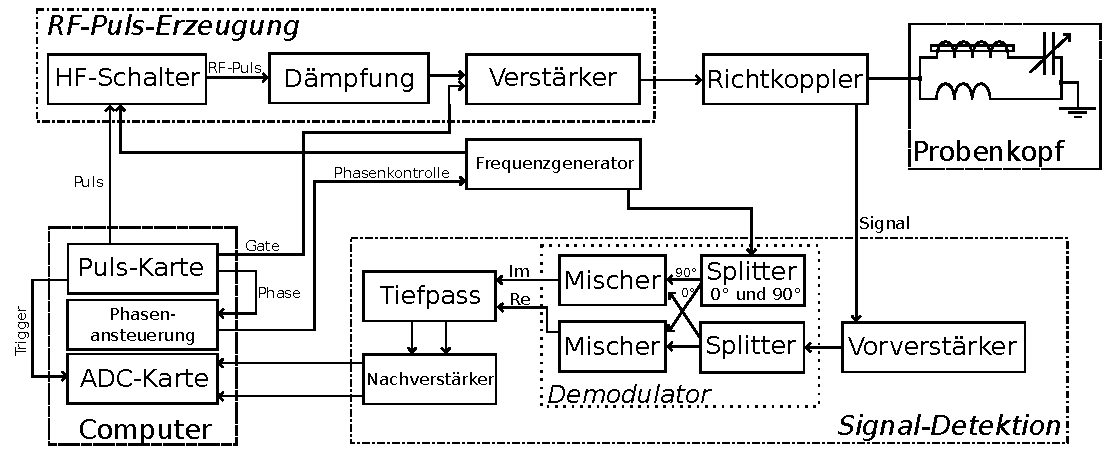
\includegraphics[width=\textwidth]{graphics/joachim/aufbau.pdf} 
	\end{center}
	\caption{Skizzierter Aufbau eines NMR-Spektrometers. Abbildung aus \cite[S. 29]{lueg_implementierung_2016}} \label{fig:exp:aufbau}
\end{figure}

Die Beschreibung nachvollzieht den Aufbau entlang des Signalwegs. Die Steuerung aller Messungen geschieht über einen Computer, der mit der in Python geschriebenen Software DAMARIS (Darmstadt Magnetic Resonance Instrument Software \cite{gadke_damaris_2007}) ausgestattet ist. Diese erlaubt es, Messprogramme zu definieren, mit Hilfe von Pythons serial-Schnittstelle die Verbindung zu verschiedenen Geräten herzustellen, und die produzierten Signale aufzunehmen, anzuzeigen und zur Weiterverarbeitung zu speichern.

Durchgängig läuft ein Frequenzgenerator vom Typ PTS 310, dessen Frequenz auf die Larmorfrequenz des zu untersuchenden Kerns im jeweiligen Magneten eingestellt ist. Ist diese Frequenz nicht bekannt, empfiehlt sich in der Regel das Aufnehmen eines Spektrums von einer Flüssigkeit oder Lösung, die den gewünschten Kern enthält. Aufgrund der geringen Breite des Flüssigkeitsspektrum lässt sich so die magnetfeldabhängige Larmorfrequenz bestimmen.

Soll ein Puls an den Probenkopf gesandt werden, setzt DAMARIS über eine 24-bit-Puls-Karte für die Dauer des Pulses ein Bit auf 1, was mit Hilfe eines HF-Schalters aus dem kontinuierlichen Signal des Frequenzgenerators einen Puls mit der gewünschten Länge ausschneidet.

Dieser Puls wird nun gedämpft. Über diese variable Dämpfung lässt sich die Stärke des Pulses und damit aufgrund der Beziehung $B_\text{Spule} \propto I_\text{Puls}$ das in der Probenspule entstehende Magnetfeld variieren. Dieses wiederum ist nach Formel \eqref{eqn:theo:pulslaenge} entscheidend für die Länge aller Pulse. Es soll die Näherung gelten, dass die während der Pulse stattfindende Dynamik vernachlässigbar ist. Dafür sollte die Dämpfung so eingestellt werden, dass sich die Länge eines Invertierungspulses im Bereich weniger Mikrosekunden befindet.

Der so gedämpfte Puls wird dann mit einem Verstärker der Firma Dressler mit $\SI{2}{\kilo\watt}$ Leistung um einen konstanten Faktor verstärkt und trifft dann über einen Richtkoppler auf den Probenkopf. Der Richtkoppler verhindert dabei, dass der leistungsstarke Puls auf die Detektionselektronik trifft, welche für die Verstärkung \emph{schwacher} Signale ausgelegt ist und entsprechend empfindlich ist.

Das nach dem Puls vom Probenkopf zurückgegebene Signal wird vom Richtkoppler zur Signal-Detektion geleitet. Es wird zunächst von einem Vorverstärker verstärkt, ehe es gesplittet wird. Beide Teile werden mit der vom Frequenzgenerator erzeugten Sinus-Schwingung, welche die Larmorfrequenz hat, gemischt; eine der Schwingungen ist jedoch um $\SI{90}{^\circ}$ phasenverschoben. Die so entstehenden Signale werden Real- und Imaginärteil des Signals genannt. Zusätzlich können beide Teile um eine konstante Phase verschoben werden. Diese lässt sich wiederum über DAMARIS mit einer Phasenansteuerungs-Karte einstellen.

Im nachfolgenden Tiefpass werden alle hochfrequenten Teile des Signals abgeschnitten, sodass nur die durch das Mischen entstandende Differenz $\Delta \omega = \omega_L - \omega_\text{Signal}$ verbleibt. Es lässt sich die Cutoff-Frequenz sowie die Amplitude und der Offset beider Einzelsignale einstellen. Die letzteren Beiden sollten so gewählt sein, dass der Offset Null ist und beide Signale die gleiche Amplitude haben.


Beide Signale werden mit einem Nachverstärker verstärkt, ehe sie von einer ADC-Karte (engl. ADC: Analog-Digital-Konverter) des Computers in Form von Amp\-li\-tu\-den-Wer\-ten in der gesetzten Frequenz von bis zu $\SI{10}{MHz}$ aufgenommen werden. Die ADC-Karte wird dabei über die Puls-Karte mit einem Trigger geschaltet. Dies kann notwendig sein, da vor dem eigentlichen Signal noch unerwünschte Effekte, wie zum Beispiel ein Nachschwingen der Probenspule, auftreten können. Um diese abzuschneiden, kann das Aufnehmen des Signals um eine festgelegte Trigger-Zeit verzögert werden.

Für mehr Informationen zu den hier beschrieben Aufbauten können \cite{lueg_implementierung_2016} und \cite{tilly_master} herangezogen werden.



\section{Weiterverarbeitung der Signale} \label{section:exp:weiterverarbeitung}

Alle so aufgenommen Daten bestehen aus einem Zeitpunkt $t$ und dem zugehörigen Amplitudenwert von Real- und Imaginärteil. Werden Messungen wie eine $T_1$-, $T_2$- oder $F_2$-Messung durchgeführt, ergeben sich variablenabhängige Messreihen. Es wird diese Variable (z.B. Evolutions- oder Mischzeit) meist logarithmisch gegen das Maximum des Realteils der jeweiligen Messung aufgetragen; dann können die Daten analysiert werden. Um ein möglichst großes Realteil-Signal am Ort $t_\text{Max}$ des Maximums zu gewährleisten, sollte dort der Imaginärteil einen Nulldurchgang aufweisen. Dies lässt sich mit einer entsprechenden Einstellung der Phase über die Phasenansteuerungs-Karte erreichen.

Sollen Spektren untersucht werden, wird das Zeitsignal fouriertranformiert. Für eine hohe Auflösung sollte ein möglichst langes Zeitsignal aufgenommen werden; für eine große Spanne ein Zeitsignal mit möglichst hoher Frequenz der ADC-Karte.



\section{Probenköpfe} \label{section:exp:probenkoepfe}

NMR-Messungen bei mehreren Hundert Grad Celsius durchzuführen, kann sich mitunter als eine Herausforderung gestalten. Lötzinne, die häufig verwendet werden um die Resonanzspule an dem Probenkopf anzubringen, schmelzen je nach Art bei weniger als $\SI{200}{\degreeCelsius}$. Aber auch Tuningkondensator und Matchingspule sowie der für die Resonanzspule verwendete Draht sind häufig nur für bestimmte Temperaturen ausgelegt. Zudem ist es offensichtlich, dass für höhere Temperaturen eine gute Isolierung und gegebenenfalls Kühlung des Probenkopfs gegeben sein muss, befindet er doch in direkter Umgebung des mit flüssigem Helium gekühlten Magneten.

Für solche Anwendungen ist also ein spezieller Probenkopf notwendig, welcher in Form des Hochtemperaturprobenkopfs (intern als „Ofen“ bezeichnet) als eine Spezialanfertigung realisiert wurde. Dessen Konstruktionszeichnung ist in Abbildung \ref{fig:exp:ofen_aufbau} zu sehen; eine detaillierte Beschreibung findet sich in \cite{tilly_master}.

\begin{sidewaysfigure}
	\begin{figure}[H]
		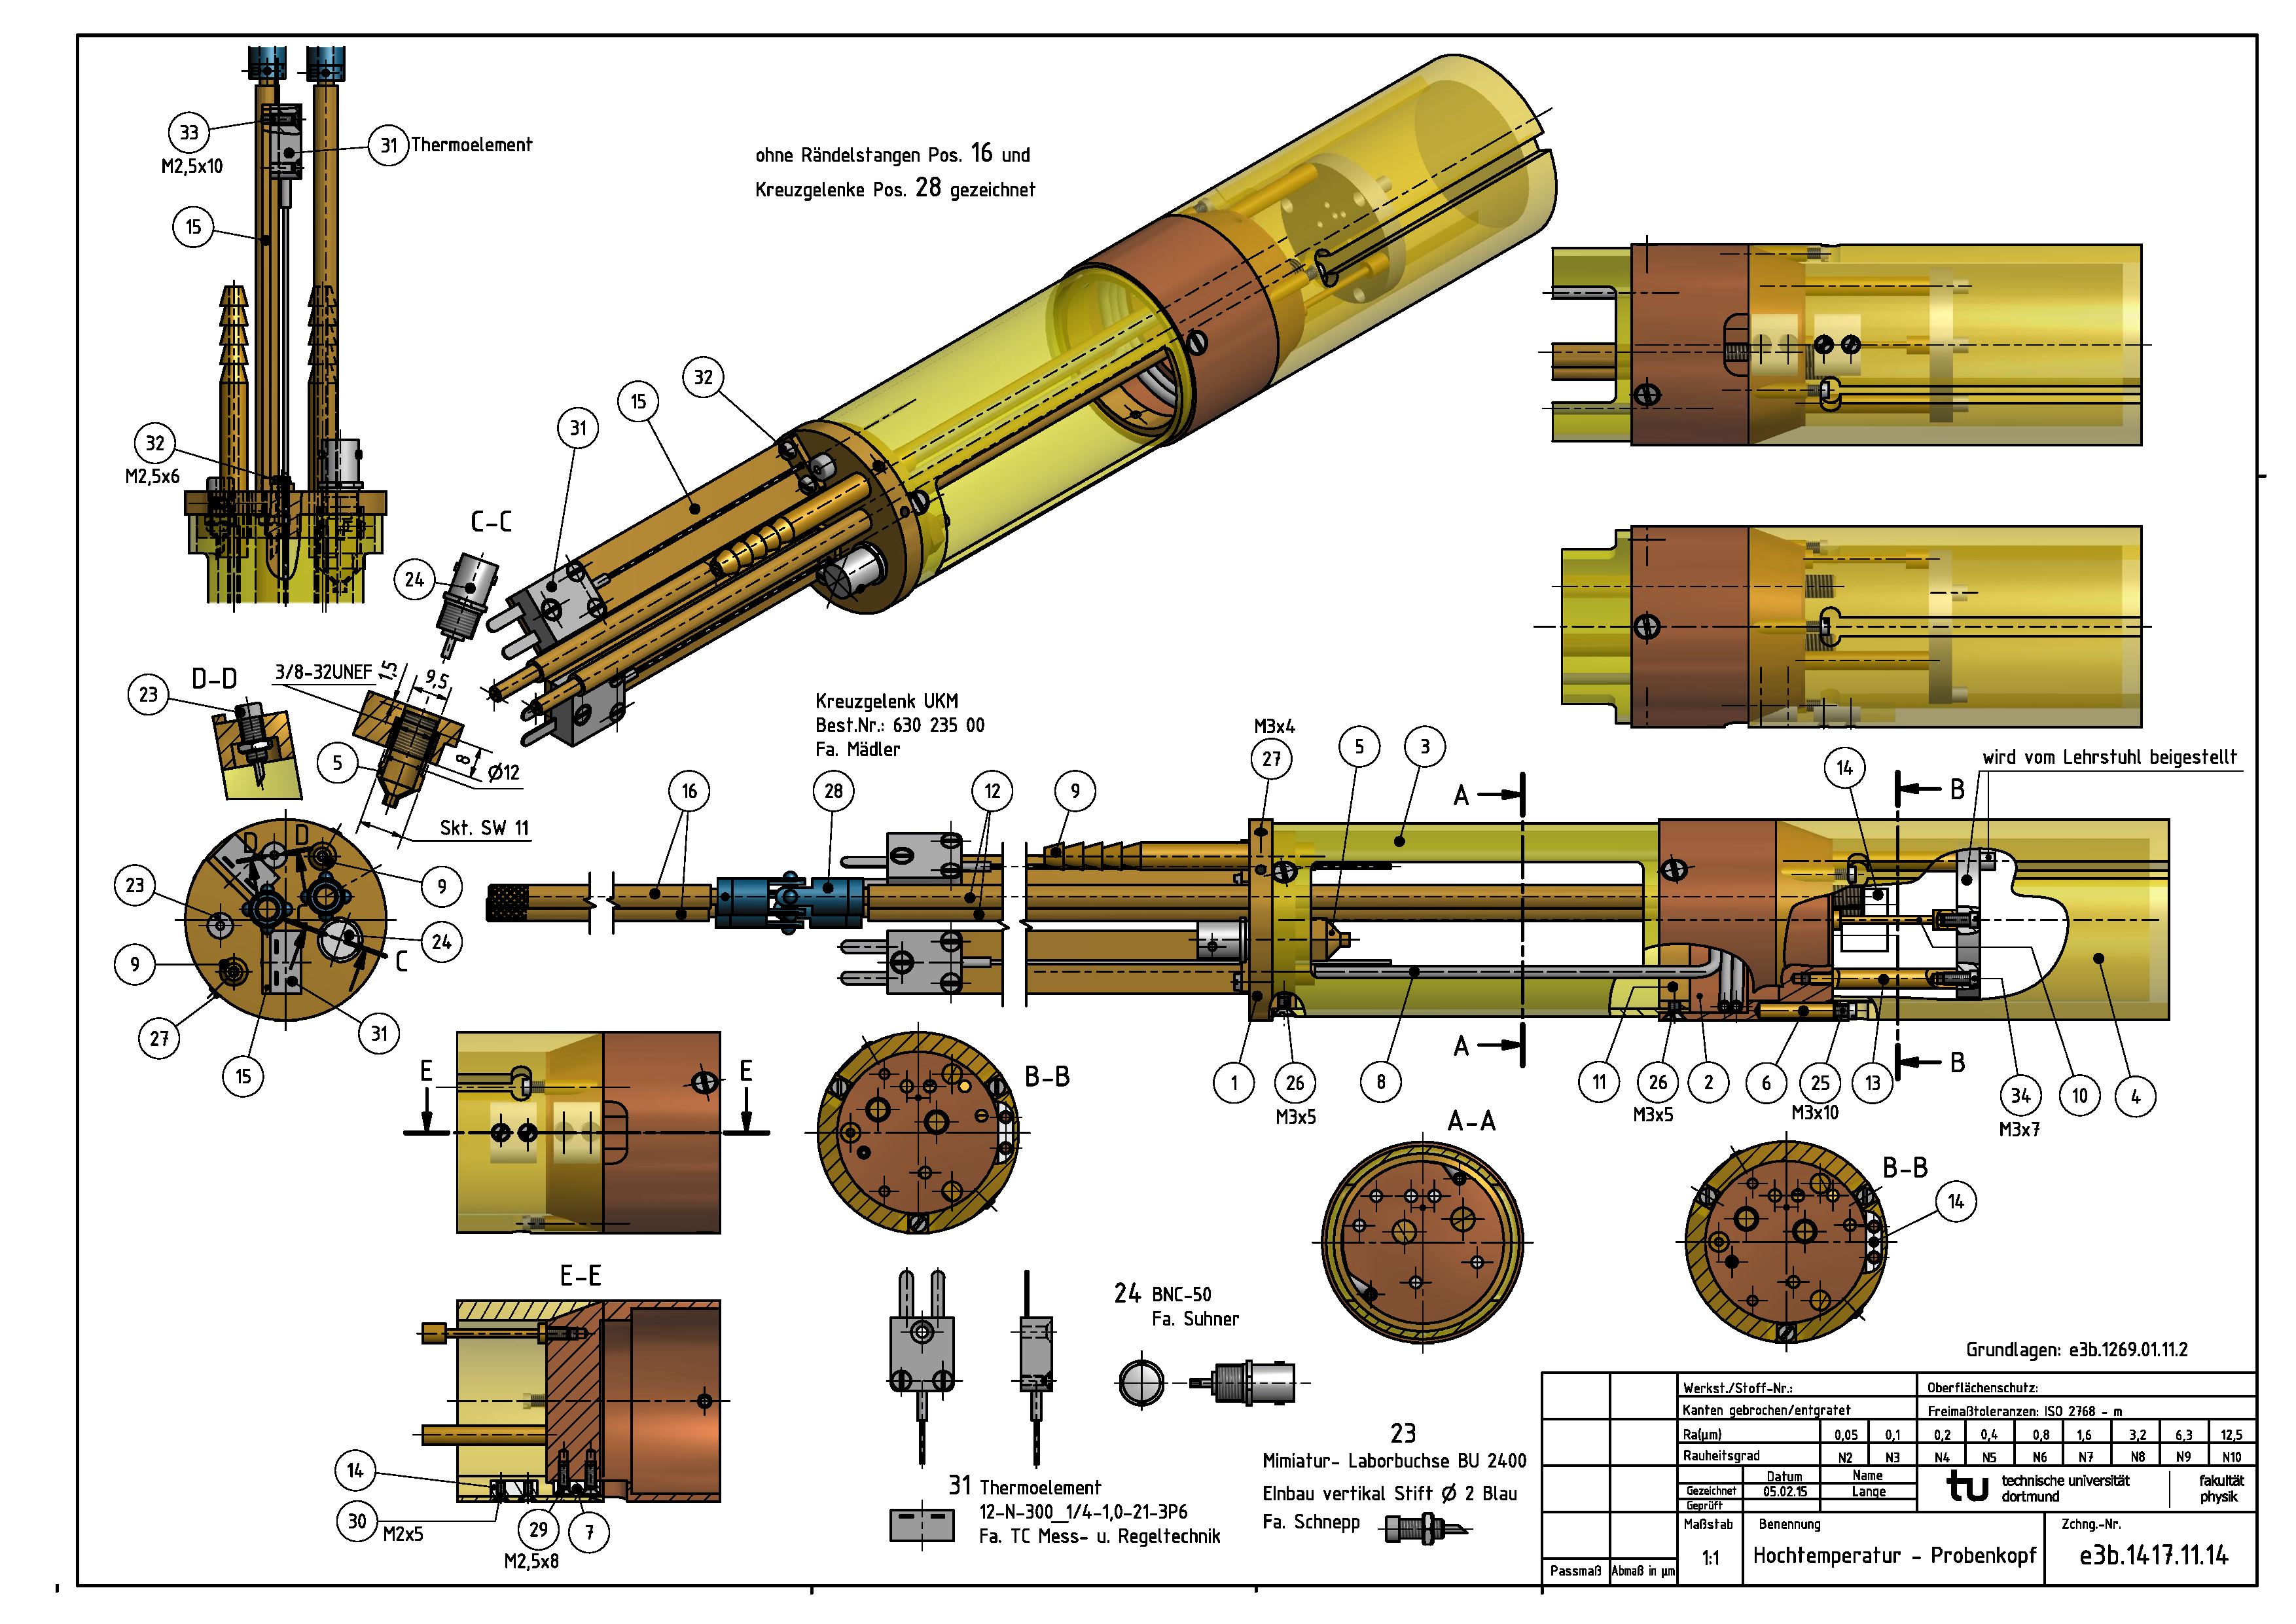
\includegraphics[width=1.05\textheight]{graphics/ofen/ofen_aufbau2.pdf}
		\caption{Konstruktionszeichnung des Hochtemperaturprobenkopfes \cite{Rudloff_blue_print}.}
		\label{fig:exp:ofen_aufbau}
	\end{figure}
\end{sidewaysfigure}

Er lässt sich grob in drei Teilen beschreiben: Im oberen Drittel befindet sich der Schwingkreis mit der Probe, eine Vorrichtung, um diese zu erwärmen, sowie die dazugehörige notwendige thermische Isolation. Am unteren Drittel werden alle notwendigen Verbindungen angeschlossen; das mittlere Drittel verbindet beides und beherbergt einen Netzfilter.

Um Temperaturen von bis zu $\SI{1100}{K}$ erreichen zu können, wird ein Heizdraht aus einer FeCrAl-Legierung verwendet. Dieser ist bifilar über einen Hartkeramik-Hohlzylinder gewickelt, um möglichst wenig störende Magnetfelder entstehen zu lassen -- gerade in direkter Umgebung der Probe. Diese Vorrichtung ist im Deckel untergebracht, der sich über die aus Platin bestehende Probenspule stülpen lässt.

Um die entstehende Hitze möglichst gut nach außen hin zu isolieren, ist dieser Aufbau von poröser Keramik umgeben -- sowohl innerhalb des Deckels als auch zwischen Probenspule und Rest des Probenkopfes. Bei letzterem ist zudem eine weitere Scheibe aus dichter Keramik vorhanden. Für die Probenspule und Temperaturfühler sind Bohrungen in den Keramikscheiben vorhanden, über die sie mit dem Rest des Probenkopfes verbunden werden können.

Darunter befindet sich der Schwingkreis der Probenspule. Sowohl eine Matchingspule als auch ein variabler Kondensator und eine Halterung für einen wechselbaren Kondensator sind vorhanden. Es lassen sich Kondensatoren mit verschiedenen Kapazitäten in der Halterung anbringen; zusammen mit dem variablen Kondensator kann so für die Resonanzfrequenz eine Spanne von $\SI{63,6}{MHz}$ bis $\SI{168,9}{MHz}$ (mit Unterbrechungen) abgedeckt werden. Darunter befindet sich die Möglichkeit für eine Wasserkühlung.

Der sich in dem Verbindungsteil befindliche Netzfilter soll den Heizstrom von störenden Anteilen befreien. Dazu wird eine Spule mit eisernem Kern verwendet. Während diese Drossel den Probenkopf in der Vergangenheit genau im Hauptfeld des Magneten gehalten hatte, ist dies jetzt nicht mehr der Fall, was eine hochqualitative Messung sehr schwer macht. Da zudem unerwünschte Einflüsse durch das zusätzliche Magnetfeld zu befürchten sind, liegt die Idee nahe, den vorliegenden Aufbau zu ändern. Eine mögliche Anpassung könnte sein, den Netzfilter außerhalb des Probenkopfes anzubringen und die Positionierung des Probenkopfes im Hauptfeld des Magneten durch eine zusätzliche Halterung zu gewährleisten.

Um den Aufbau zu betreiben, sind im letzten Drittel eine Reihe von Anschlüssen vorhanden:
\begin{itemize}
	\item Ein BNC-Anschluss der vom Richtkoppler kommend zum Schwingkreis führt,
	\item Bohrungen für die beiden Thermoelemente, welche von einem Temperatur-Controller ausgelesen werden,
	\item ein Anschluss für den Heizstrom, welcher von einem Temperatur-Controller bereitgestellt wird,
	\item je eine Rändelstange für die Einstellung von Matching\-spu\-le und Tuningkondensator,
	\item Anschlüsse für Zu- und Abflussschläuche für das Kühlwasser. Der Zufluss kann mit einem Wasserhahn gespeist werden.
\end{itemize}

„Reguläre“ Probenköpfe sind im Vergleich recht einfach gehalten. Da die Temperatursteuerung meist durch den Kryostaten geleistet wird, fallen die Heizeinheit, Isolation, Wasserkühlung und Netzfilter heraus, und es bleiben nur Schwingkreis und Temperaturfühler. In dem hier verwendeten Probenkopf P1 ist zudem keine Matchingspule vorhanden, sodass sich das Abstimmen des Probenkopfs deutlich umständlicher gestaltet und durch eine sehr genaue (und dadurch aufwändigere) Wickelung der Probenspule geleistet werden muss.




\section{Temperaturkontrolle} \label{section:exp:temperaturkontrolle}

Um häufig gewünschte temperaturabhängige Messungen durchführen zu können, lassen sich über Python-Skripte Temperatur-Controller, wie zum Beispiel die hier verwendeten Lakeshore-Einheiten, benutzen. So wird ein Auslesen der aktuellen Temperatur sowie das Setzen einer Soll-Temperatur ermöglicht. Der Temperatur-Controller wiederum steuert Temperatureinheiten im Probenkopf (im Falle des Hochtemperaturprobenkopfs) oder im Kryostaten (im Falle des Probenkopfs P1) an. Die aktuelle Temperatur wird über Temperaturfühler erfasst. Dabei handelt es sich im Falle des Hochtemperaturprobenkopfes um Thermoelemente vom Typ N, im Falle des Probenkopfes P1 um PT100-Elemente ***.





\section{Proben} \label{section:exp:proben}

Bei den durchgeführten Messungen wurden sechs verschiedene Proben verwendet:

\begin{table}[H]
	\centering
	\begin{tabular}{rllllllrl}
		\hline
		ID & Chemikalie & Hersteller & Datum & Glas & Form & \diameter & Foto \\ 
		\hline
		1	& CRN &	C. Zürn &	16.04.97 &	? &	gebogen & 	$\SI{6}{\milli\meter}$ &	(a) \\
2	& CRN &	J. Adam &	13.07.17 &	Duran &	gebogen & 	$\SI{6}{\milli\meter}$ &	(b) \\
3	& CRN &	J. Adam &	30.08.17 &	Duran &	gerade & 	$\SI{5}{\milli\meter}$ &	(c) \\
4	& CRN &	J. Adam &	30.08.17 &	Duran &	gebogen & 	$\SI{5}{\milli\meter}$ &	- *** \\
5	& RbCl in D$_\text{2}$O &	J. Adam &	30.08.17 &	Duran &	gerade & 	$\SI{5}{\milli\meter}$ &	(d) \\
6	& RbCl in D$_\text{2}$O &	J. Adam &	30.08.17 &	Duran &	gebogen & 	$\SI{5}{\milli\meter}$ &	(d) \\ \hline
	\end{tabular} 
	\caption{In dieser Arbeit verwendete Proben. CRN bezeichnet dabei 2Ca(NO$_\text{3}$)$_\text{2}$-3RbNO$_\text{3}$. \label{tab:exp:proben}}
\end{table}

\begin{figure}[H]
	\centering
	\begin{subfigure}{.24\textwidth}
		\centering
		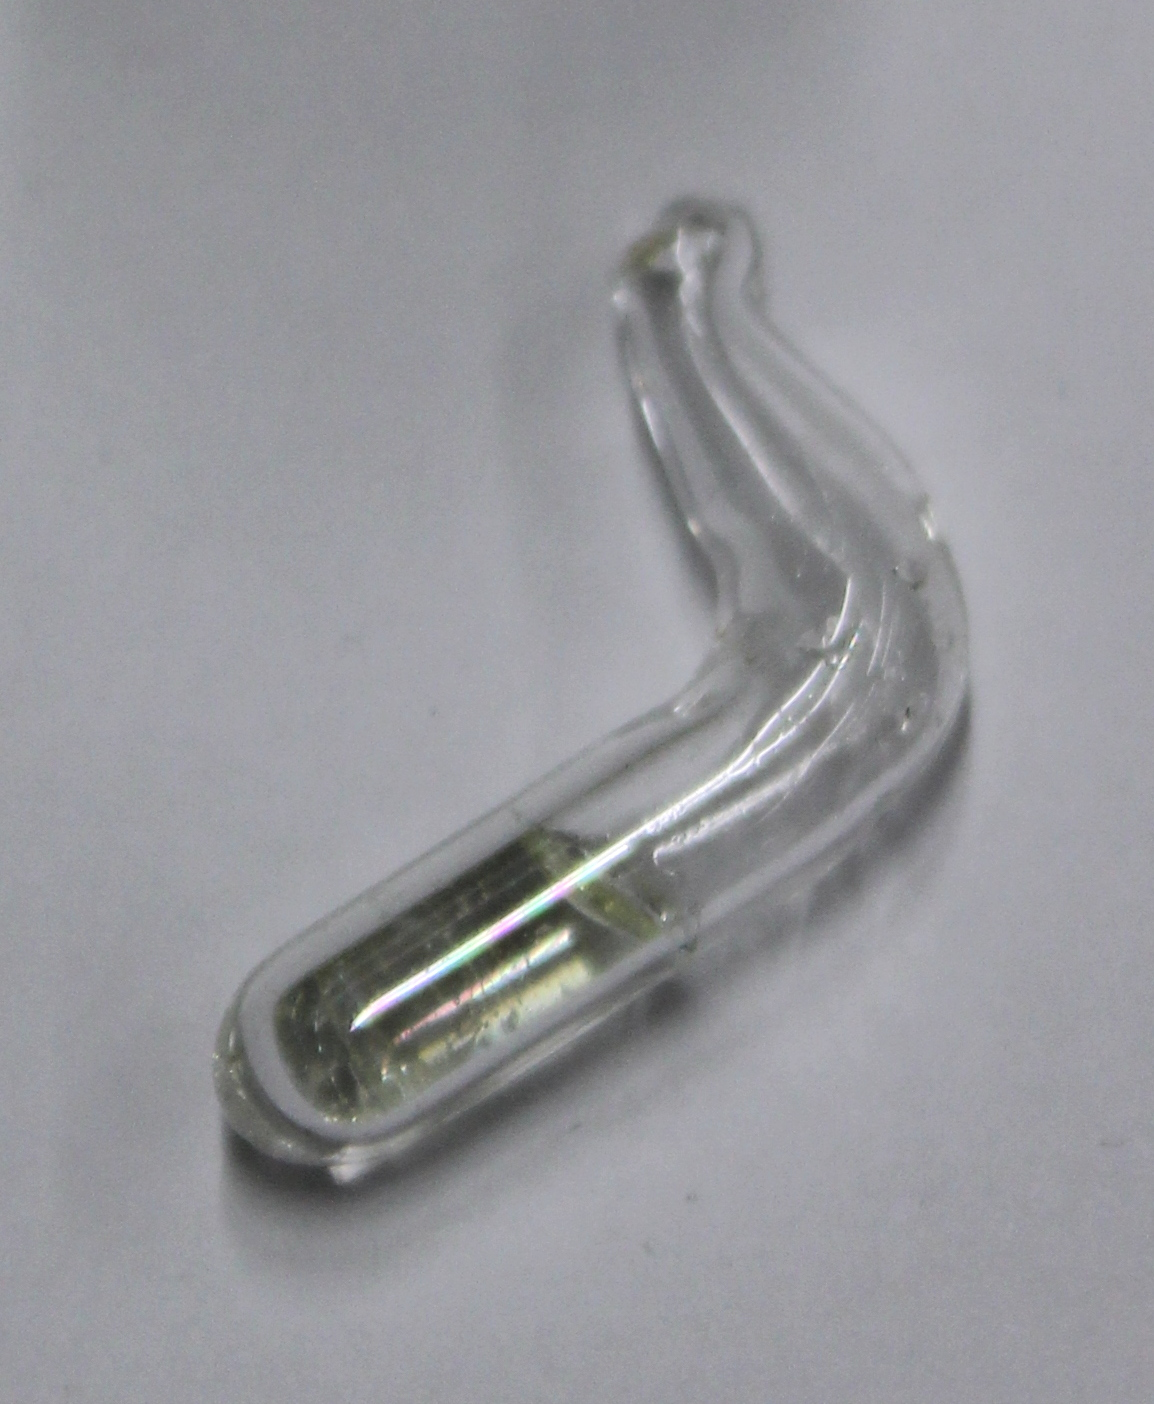
\includegraphics[width=0.95\textwidth]{graphics/proben/CRN_zuern.jpg}
		\caption{ }
		\label{fig:exp:probe_a}
	\end{subfigure}%
	\begin{subfigure}{.24\textwidth}
		\centering
		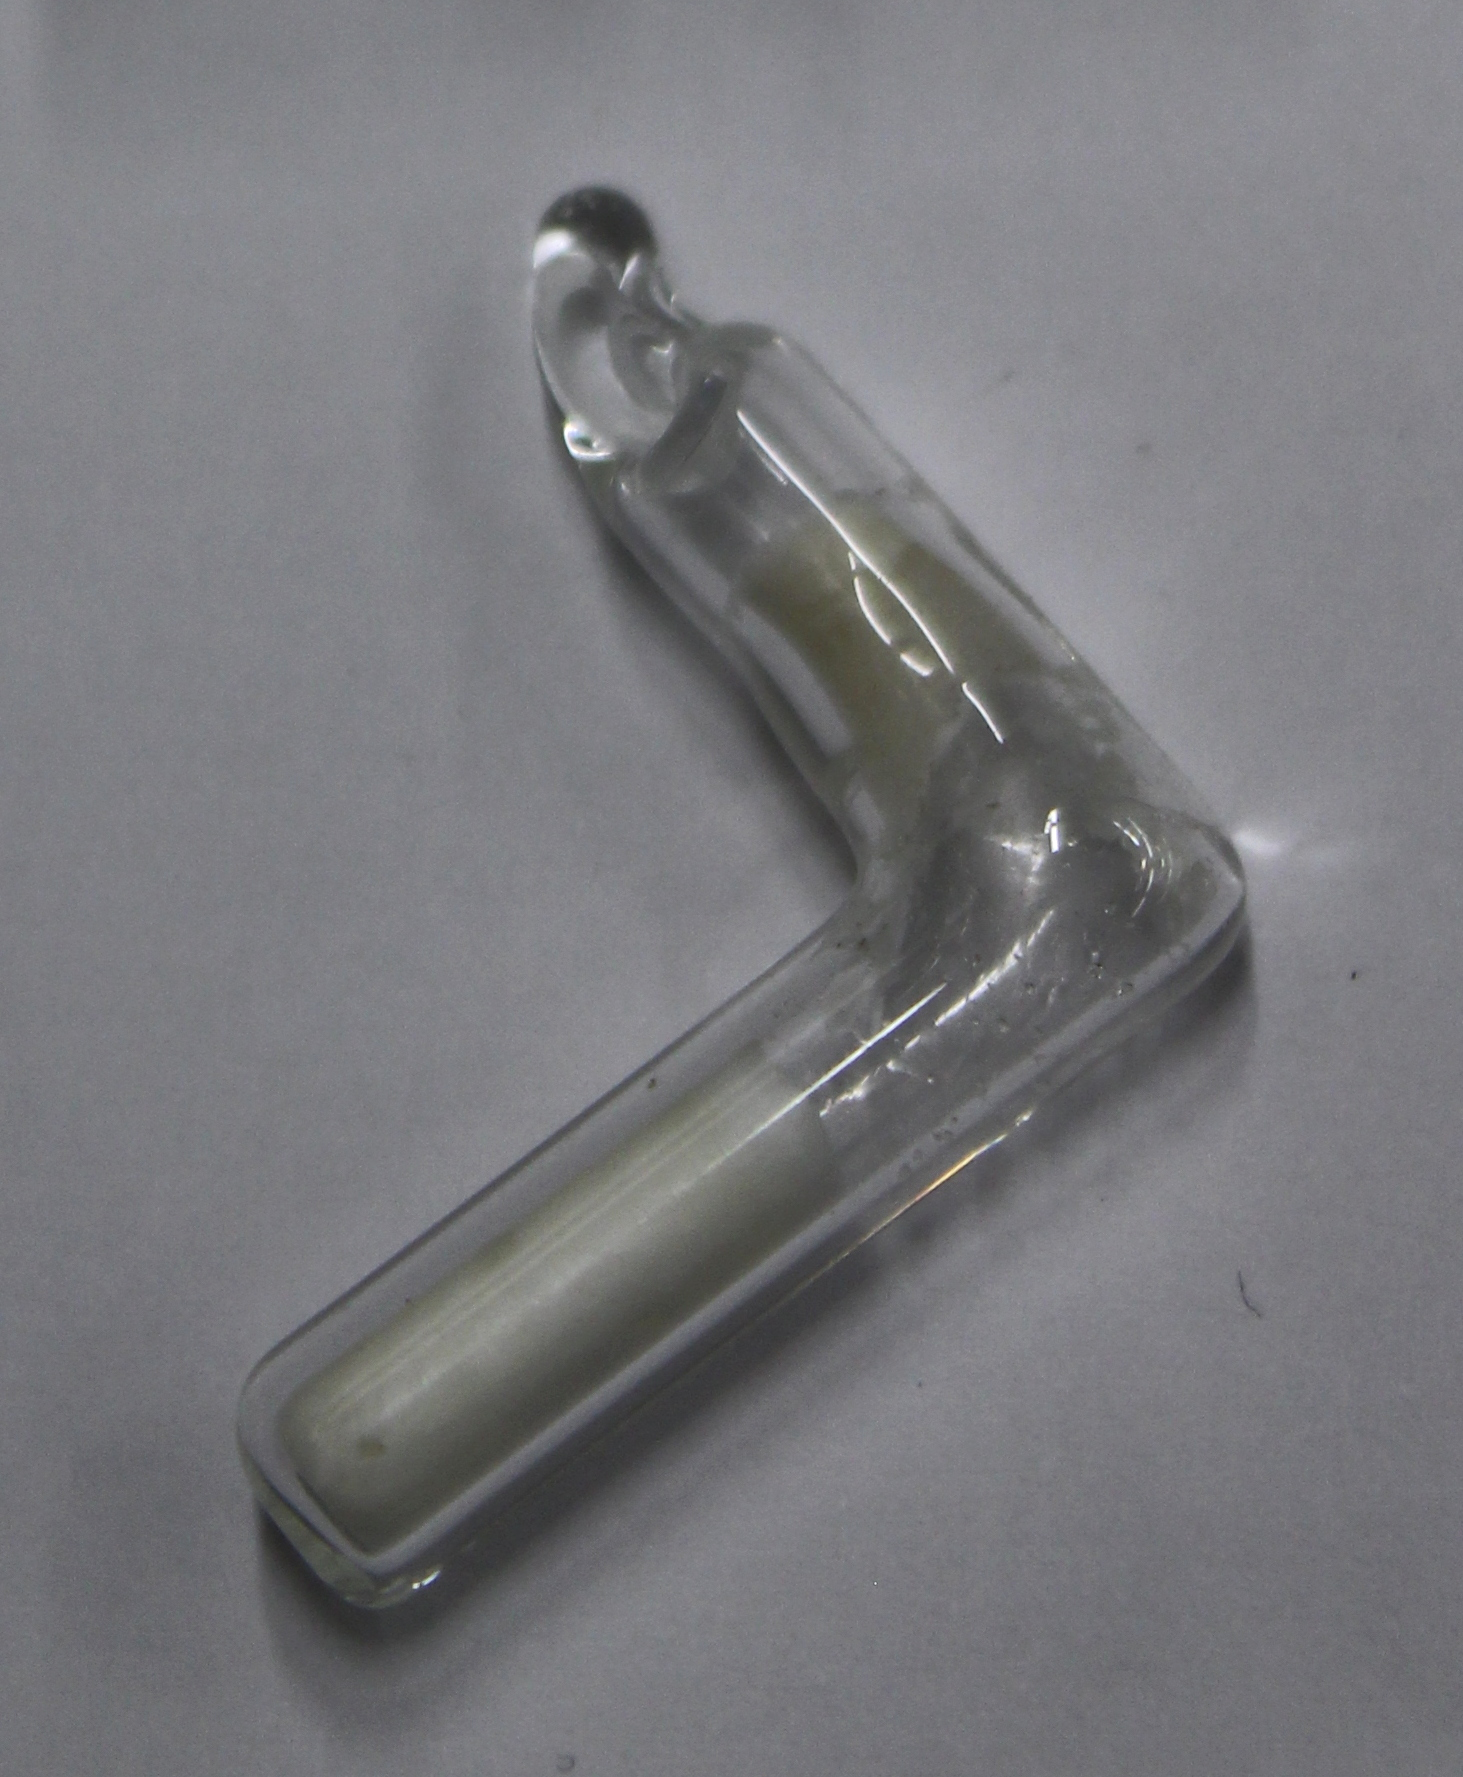
\includegraphics[width=0.95\textwidth]{graphics/proben/CRN_alt.jpg}
		\caption{ }
		\label{fig:exp:probe_b}
	\end{subfigure}
	\begin{subfigure}{.24\textwidth}
		\centering
		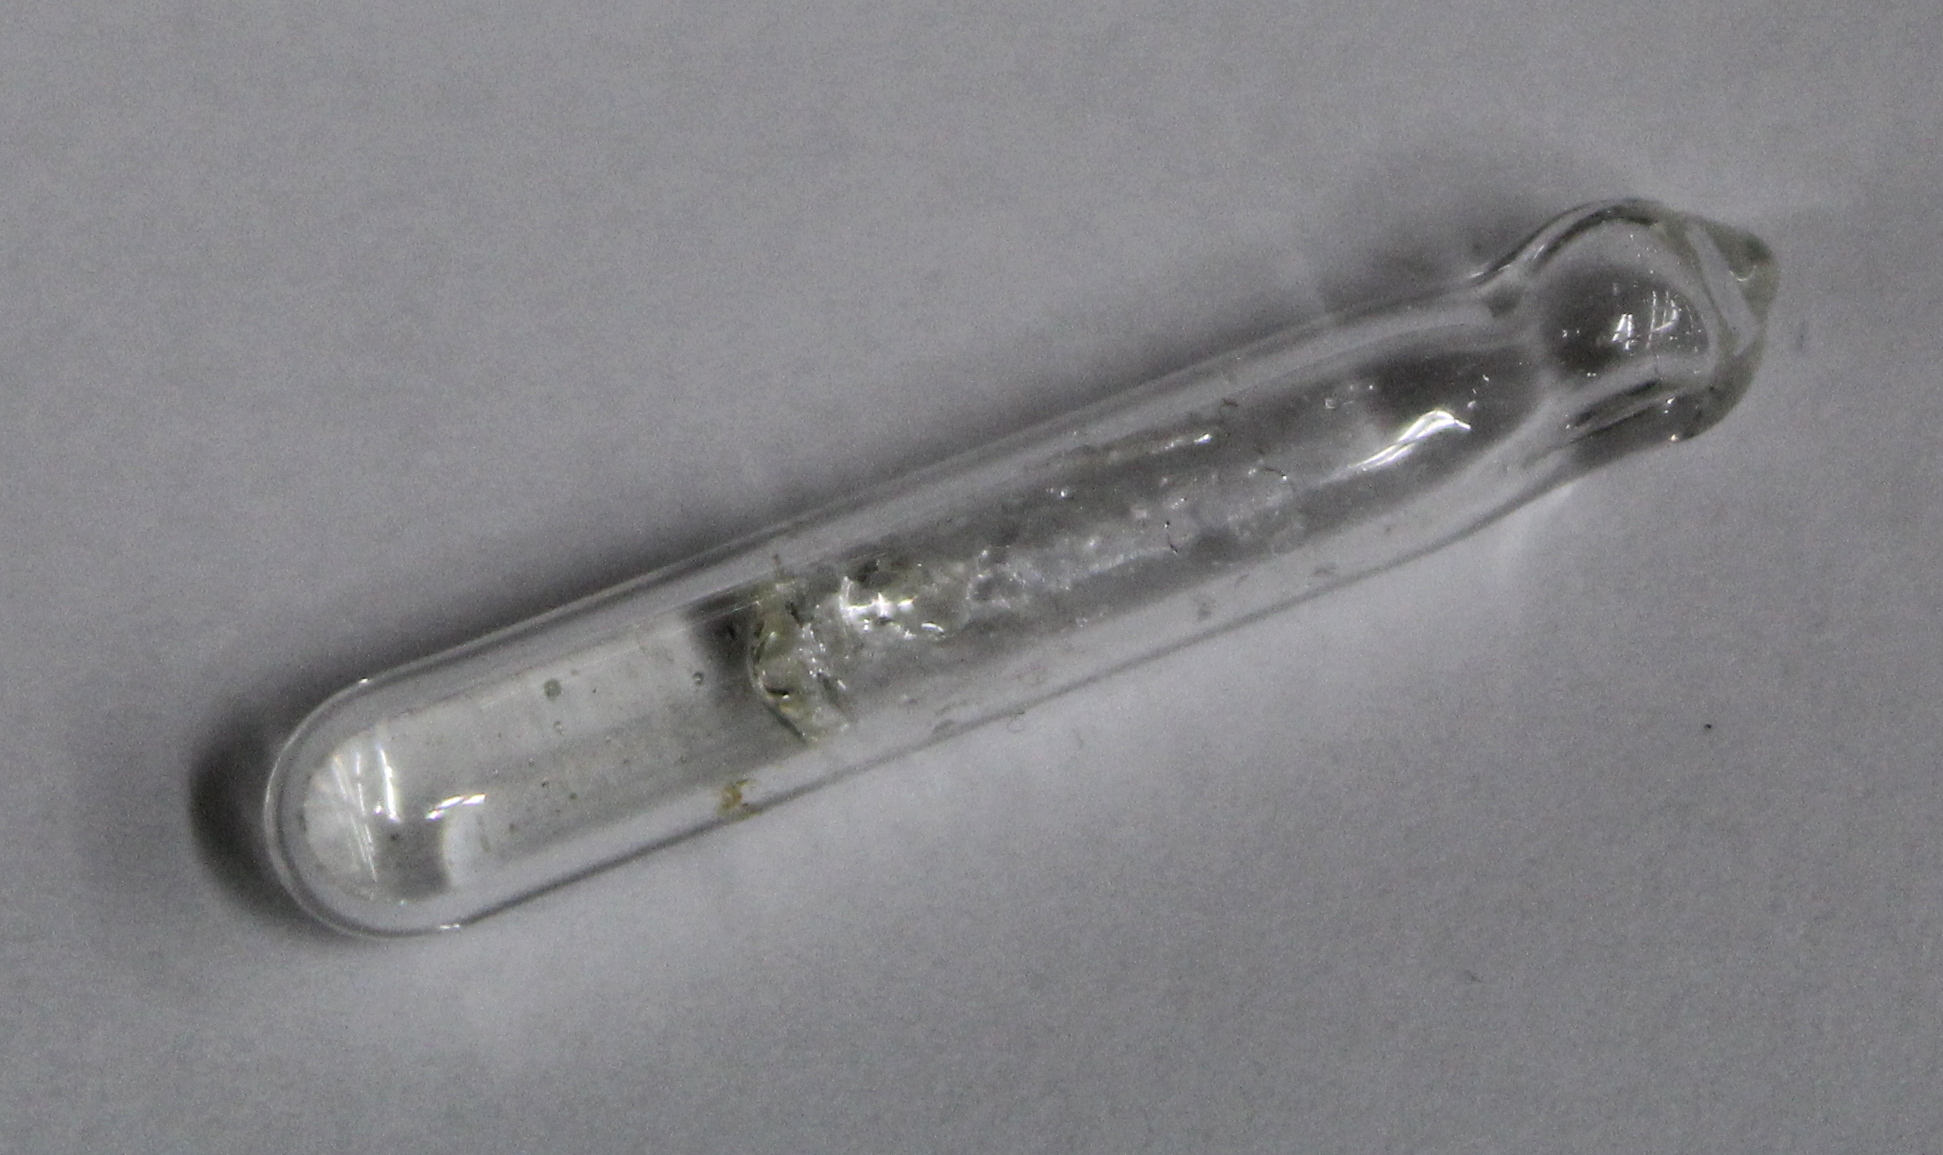
\includegraphics[width=\textwidth]{graphics/proben/CRN_neu.jpg}
		\caption{ }
		\label{fig:exp:probe_c}
	\end{subfigure}
	\begin{subfigure}{.24\textwidth}
		\centering
		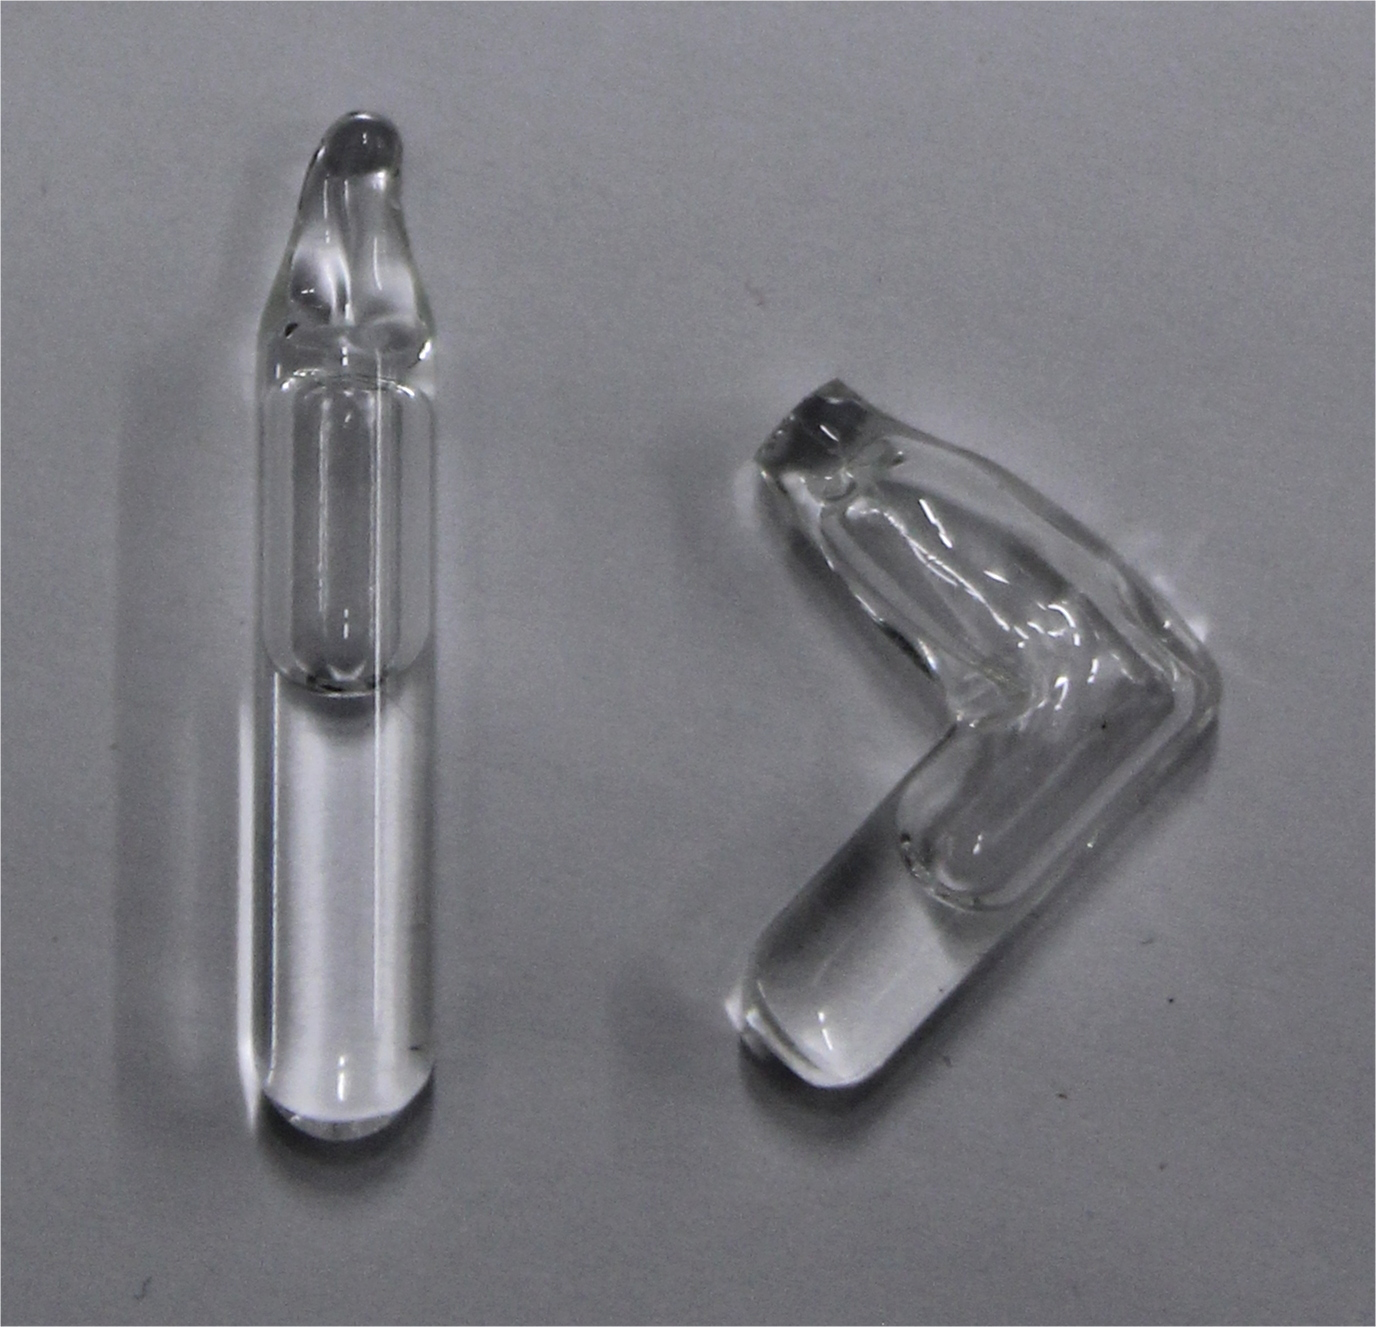
\includegraphics[width=\textwidth]{graphics/proben/RbCl_in_D20.jpg}
		\caption{ }
		\label{fig:exp:probe_d}
	\end{subfigure}
	\caption{Fotografien der verwendeten Proben. Die Merkmale finden sich in Tabelle \ref{tab:exp:proben}}
	\label{fig:exp:proben}
\end{figure}

Die Herstellung C. Zürns Probe 1 ist in \cite{zuern_arbeit} dokumentiert.

Die Proben 3 und 4 wurden für diese Arbeit angefertigt. Dafür wurde CRN (was genau für welches? ***) zu einem möglichst feinen Pulver zermörsert und ein gerades bzw. gebogenes Duran-Glas-Röhrchen gefüllt. Um störende Einflüsse von Feuchtigkeit in der Probe möglichst gut zu elimieren, wurden die Proben über Nacht bei $\SI{160}{\degreeCelsius}$ in einem evakuierten Ofen getrocknet, der im Anschluss mit Stickstoffgas gelöscht wurde.

So präpariert wurden die Proben unter Anwendung eines Freeze-Pump-Thaw-Ver\-fah\-rens von Herrn Kollman, Glasbläser der TU Dortmund, abgeschmolzen. Mit dem Verfahren soll der Probe möglichst viel Gas entzogen werden, indem sie Vakuum ausgesetzt wird. Damit die Probe aber nicht mit angesaugt wird, wird sie vor dem Abpumpen eingefroren und danach wieder getaut. Anschließend wurden die Proben durch Erhitzen geschmolzen, um sie dann in einem Glaszustand abkühlen zu lassen.

Mit dem gleichen Verfahren wurde am 13.07.2017 die Probe 2 erstellt, wobei hier die Probe \emph{vor} dem Abschmelzen in den Glaszustand gebracht wurde. Diese Probe wurde jedoch nicht verwendet, da Tests zeigten, dass sie kaum stabil im Glaszustand zu halten war sondern schnell auskristallisierte.

Zum Bestimmen der Larmorfrequenz von $^\text{87}$Rb wurden zudem zwei Proben, Proben 5 und 6, mit in D$_\text{2}$O gelöstem RbCl erstellt. Dabei wurde die gesättigte Lösung in Duran-Glas-Röhrchen eingefüllt und vor dem Abschmelzen möglichst langsam eingefroren, um ein Springen des Röhrchens durch das beim Übergang zum Eis erhöhte Volumen zu verhindern.

\chapter{Experimentelle Resultate und Analysen}
\label{chapter:experiment}

Im Folgenden sollen die im Rahmen dieser Arbeit aufgenommenen Daten vorgestellt und ausgewertet werden. Dabei lassen sich zwei separate Bemühungen unterscheiden. Zum einen wurden Untersuchungen zur Dynamik in CRN angestellt, welche zuerst präsentiert werden sollen, zum anderen wurden die Linienformänderungen in Abhängigkeit der Temperatur untersucht und mit theoretischen Überlegungen verglichen.

Im Verlauf der Auswertung werden die Daten zum Teil nach dem verwendeten Spektrometer unterschieden. Dies liegt an der unterschiedlichen Larmorfrequenzen der Apparaturen -- $\omega_{L, \text{OBI}} / 2\pi = f_{L, \text{OBI}} = \SI{97.1722}{MHz}$ im Vergleich zu $\omega_{L, \text{Bruker}} / 2\pi = f_{L, \text{Bruker}} = \SI{130.9736}{MHz}$ -- welche sich um etwa einen Faktor $\SI{1.35}{}$ unterscheiden. Dies ist genug, um eine deutliche Auswirkung in den Daten beobachten zu können.

Bei beiden Spektrometern wurden für die grundlegenden Parameter bei allen Messungen etwa die gleichen Einstellungen verwendet: Für das OBI-Spektrometer wurde die Dauer eines $\SI{180}{\degree}$-Pulses auf einen Wert zwischen $\SI{6.5}{\micro s}$ und $\SI{7.1}{\micro s}$ gesetzt, beim Bruker-Spektrometer auf $\SI{5.2}{\micro s}$. Dabei wurde selektiv die Zentrallinie angeregt. Das bedeutet, dass das $^\text{87}$Rb-NMR-Spektrum zu breit ist, als dass es nicht-selektiv angeregt werden könnte, und da es sich bei $^\text{87}$Rb um einen Kern mit halb-zahligen Spin handelt, wird nur der Übergang $-\sfrac{1}{2} \leftrightarrow \sfrac{1}{2}$ -- welcher im Spektrum als sogenannte Zentrallinie zu sehen ist -- angeregt.

Die Evolutionszeit $t_p$ der Echos beträgt in den meisten Fällen $\SI{15}{\micro s}$ und nie mehr als $\SI{20}{\micro s}$. Die Wiederholungszeit, also die Zeit zwischen zwei Pulsfolgen, beträgt zwischen $\SI{10}{\milli s}$ und $\SI{50}{\milli s}$. Dies soll dafür sorgen, dass die Magnetisierung nach jeder Pulsfolge wieder in den Ausgangszustand jeder Pulsfolge, der Gleichgewichtsmagnetisierung, zurückkehren kann. Dafür sollte ein Vielfaches der $T_1$-Zeitkonstante gewartet werden.

Der mit dem OBI-Spektrometer abgedeckte Temperaturbereich reicht von $\SI{230}{\kelvin}$ bis $\SI{435}{\kelvin}$, während sich der Temperaturbereich des Bruker-Spektrometers auf den Bereich von $\SI{310}{\kelvin}$ bis $\SI{390}{\kelvin}$ beschränkt.

Alle beschriebenen Fits wurden durch eine least-squares-Methode mit Hilfe von Python-Skripten, welche \texttt{scipy.optimize}- oder \texttt{lmfit}-Routinen verwenden, erstellt.


\section{Bestimmung von $T_1$ und $T_2$} \label{section:res:T_1}

Vor dem Beginn jeder NMR-Messung ist es sinnvoll, $T_1$, die Zeitkonstante der longitudinalen Relaxation, im zu untersuchenden Temperaturgebiet zu vermessen. Dies ist hilfreich, um wichtige Parameter der Messungen abzustecken und mögliche Hindernisse im Vorhinein abschätzen zu können. So sollte zwischen allen Messungen eine Zeit von mindestens $4 T_1$ gewartet werden um sicherzugehen, dass sich die Magnetisierung in guter Näherung wieder im Gleichgewichtszustand befindet -- wird $T_1$ also im Laufe der Messung bei anderen Temperaturen länger, muss hierauf Rücksicht genommen werden. Wird $T_1$ auf der anderen Seite sehr kurz, kehrt die Magnetisierung sehr schnell in den Gleichgewichtszustand zurück und lassen dem Experimentierenden daher nur ein kleines Fenster, in dem Untersuchungen durchgeführt werden können. Hinzu kommt, dass der Temperaturverlauf von $T_1$ nach Formel \eqref{eqn:bpp} wertvolle Information über die Dynamik in der untersuchten Probe liefern kann. Zuletzt bietet diese recht einfache und reproduzierbare Messung die Möglichkeit, das Spektrometer und die Probe auf Übereinstimmung mit Literaturdaten hin zu überprüfen. Daher wurden zu allen untersuchten Temperaturen $T_1$-Messungen aufgenommen.

Zur Bestimmung von $T_1$ wurde eine Invertierungs-Pulsfolge mit Hahn-Echo verwendet. Repräsentative Rohdaten einer solchen Messung sind in Abbildung \ref{fig:res:T_1_roh} zu sehen. An die Daten wurden Fits mit $T_1$ und $\beta$ als freien Parametern entsprechend Gleichung \eqref{eqn:theo:T_1_fit} angelegt -- diese sind als Linien dargestellt. Die Daten wurden hier zudem mit $M_{T_1}(0) = -1$ und $M_{T_1}(\infty) = 1$ normiert, um einen besseren Vergleich zuzulassen. Es ist zu erkennen, dass die Fits eine gute Repräsentation der Daten ermöglichen.
\begin{figure}
	\begin{center}
		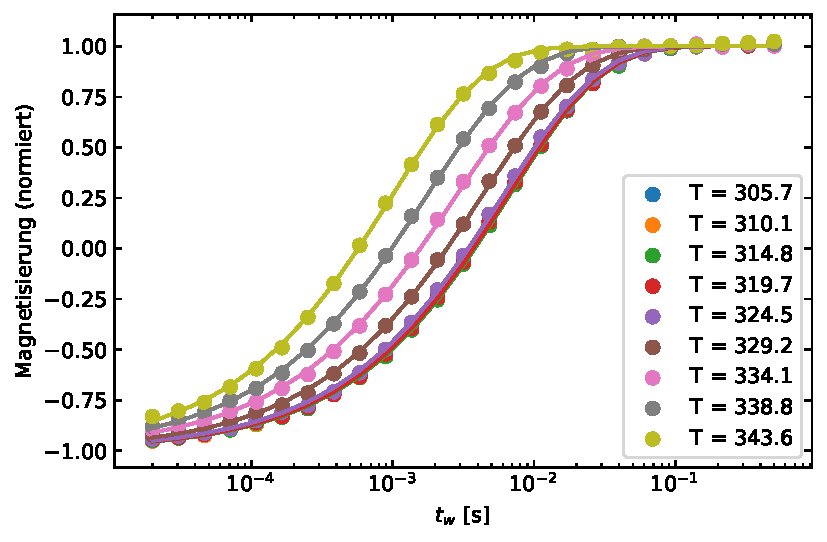
\includegraphics[width=.8\textwidth]{graphics/plot/t1_roh3.pdf}
	\end{center}
	\caption{Aufbaukurven der longitudinalen Magnetisierung zur Bestimmung von $T_1$, aufgenommen am OBI-Spektrometer mit $\omega_{L, \text{OBI}} = 2\pi \cdot \SI{97.1722}{MHz}$. Linien stellen Kohlrausch-Fits an die Datenpunkte dar. Die Daten wurden mit $M_{T_1}(0) = -1$ und $M_{T_1}(\infty) = 1$ der Fits normiert.} \label{fig:res:T_1_roh}
\end{figure}

Während sich die Kurven zwischen $\SI{305}{\kelvin}$ und $\SI{325}{\kelvin}$ sehr ähneln, verschieben sich die Kurven und damit auch die $T_1$-Werte bei höheren Temperaturen zu kürzeren Zeiten.

Dies lässt sich auch in der Gesamtübersicht aller aufgenommenen $T_1$-Daten in Abbildung \ref{fig:res:T_1} erkennen. Während die $T_1$-Zeiten bei Temperaturen von $\SI{250}{\kelvin}$ bis $\SI{325}{\kelvin}$ nahezu unverändert im unteren Millisekunden-Bereich liegen, verkürzen sie sich bei steigenden Temperaturen bis in den zweistelligen Mikrosekunden-Bereich. Es ist ein $T_1$-Minimum bei etwa $\SI{410}{\kelvin}$ mit einem Wert von ungefähr $\SI{5}{\micro s}$ auszumachen, ehe die $T_1$-Zeiten wieder länger werden.
\begin{figure}
	\begin{center}
		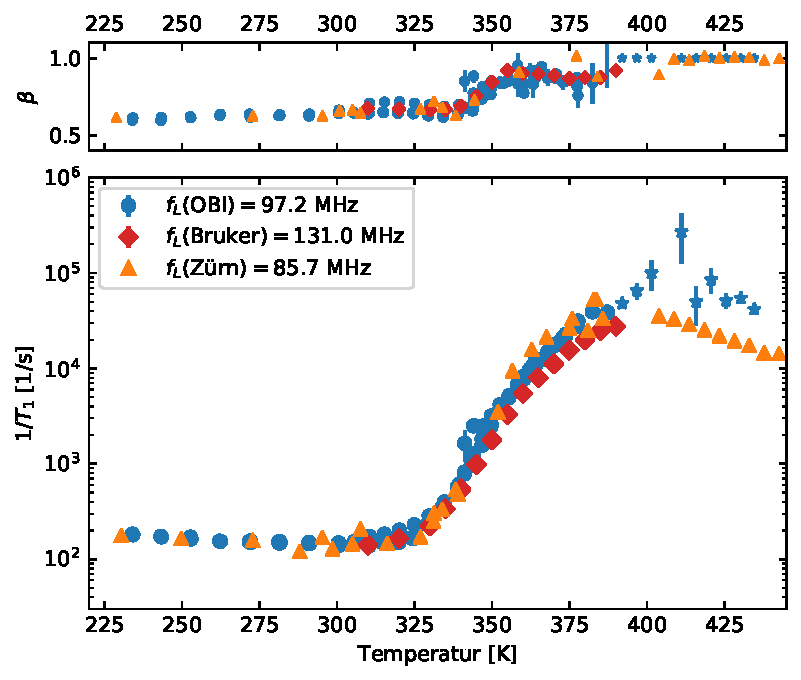
\includegraphics[width=\textwidth]{graphics/plot/t1.pdf}
	\end{center}
	\caption{$T_1$ und $\beta$ aus Fits nach Gleichung \eqref{eqn:theo:T_1_fit}. Blaue und rote Symbole zeigen die am OBI- bzw. Bruker-Spektrometer aufgenommen Daten. Bei Temperaturen über $\SI{390}{\kelvin}$ wurden die $\beta$ der Fits auf $\SI{1}{}$ festgesetzt -- diese Werte wurden mit Sternen anstatt Punkten symbolisiert. Orangene Dreiecke bieten einen Vergleich mit Daten von Zürn \cite{zuern_paper}.} \label{fig:res:T_1}
\end{figure}

Während die Unsicherheiten der Fits die Größe der dargestellten Symbole meist nicht überschreiten, sind größere Schwankungen über $\SI{390}{\kelvin}$ zu erkennen. Daher wurde hier bei den Fits konstant $\beta = 1$ gesetzt -- symbolisiert durch Sterne anstatt Punkte --, um diese Schwankungen möglichst gering zu halten.

Abgesehen von dem erwähnten Temperaturbereich ist eine gute Übereinstimmung des Verlaufs der $T_1$-Daten von Zürn \cite{zuern_paper}, welche an einem Spektrometer mit einer Larmorfrequenz von $\omega_{L, \text{Zürn}} = 2\pi \cdot \SI{85.7}{MHz}$ aufgenommen wurden, zu erkennen. Die vorhandenen Differenzen könnten durch die unterschiedlichen Larmorfrequenzen der Aufbauten verursacht worden sein. Zudem sind kaum Differenzen zwischen Messungen des OBI-Spektrometers mit überlappenden Temperaturbereichen, wie sie zwischen $\SI{330}{\kelvin}$ und $\SI{370}{\kelvin}$ auftreten, zu erkennen. Dies lässt darauf schließen, dass diese Daten gut reproduzierbar sind.

Die am Bruker-Spektrometer mit $\omega_{L, \text{Bruker}} = 2\pi \cdot \SI{130.9736}{MHz}$ aufgenommenen Daten folgen dem gleichen beschriebenen Verlauf und zeigen bis auf den Temperaturbereich zwischen $\SI{360}{\kelvin}$ und $\SI{390}{\kelvin}$ keinen nennenswerte Differenzen zu den Daten von Zürn oder den Daten des OBI-Spektrometers; dort aber sind die gemessenen $T_1$-Daten zu leicht längeren Zeiten verschoben. Der Quotient der $T_1$-Zeiten der beiden Spektrometer überschreitet den Wert $\SI{2}{}$ jedoch nicht.

Im oberen Teil der Abbildung \ref{fig:res:T_1} sind die entsprechenden $\beta$ der Fits zu sehen. Von einem Wert von $\SI{0.6}{}$ bei tieferen Temperaturen steigen sie zu einem Wert von etwa $\SI{0.9}{}$ bei Temperaturen über $\SI{350}{\kelvin}$. Dies entspricht etwa den Ergebnissen von Zürn. Bei Temperaturen oberhalb von $\SI{390}{\kelvin}$ wurden die $\beta$ der Fits, wie erwähnt, auf 1 festgesetzt -- wieder durch Stern-Symbole anstatt von Punkten dargestellt. Die Messunsicherheiten, die diesen Schritt notwendig machen, stammen daher, dass mit den verwendeten Apparaturen nicht verlässlich Datenpunkte vor $\SI{10}{\micro s}$ aufgenommen werden können. Wenn die $T_1$ Zeit aber in der gleichen Größenordnung liegt und zum Zeitpunkt des $T_1$-Werts das Signal auf etwa $1/e$ abgefallen ist, ist es verständlich, dass ein Fit Schwierigkeiten bereiten kann. Lösen ließe sich dies theoretisch mit einer längeren Evolutionszeit des verwendeten Echos; dies ist aufgrund der kurzen $T_1$- und $T_2$-Zeiten in diesem Temperaturbereich jedoch nicht möglich -- das entstehende Signal ist zu klein, um effektiv vom Rauschen getrennt zu werden.

Die Unsicherheiten der mit dem Bruker-Spektrometer bestimmten $\beta$ ist vergleichsweise gering -- die Fehlerbalken überschreiten die Größe der Symbole nicht. Dies ist mit der höheren Qualität der Daten (besonders auch bei den Linienformen der Spektren in Abbildung \ref{fig:res:bruker_linienform} im Vergleich zu \ref{fig:res:spek_linienform} zu erkennen) und den niedrigeren $T_1$-Werten zu erklären.



% \section{$T_2$} \label{section:res:T_2}
\par\bigskip


Ähnlich wie $T_1$ ist auch $T_2$ eine wichtige Größe, die Parameter für folgende Messungen bestimmen kann -- so werden beispielsweise die praktikablen Längen von Pulsabständen, in denen transversale Magnetisierung vorliegt, von $T_2$ begrenzt. Zudem kann nach Formel \eqref{eqn:theo:T_2_dyn} Aufschluss über Dynamiken gegeben werden.

In Abbildung \ref{fig:res:T_2_roh} sind exemplarisch Rohdaten verschiedener Temperaturen zu sehen. Diese wurden mit einem Hahn-Echo mit $\tau = \SI{15}{\micro s}$ aufgenommen und auf den Bereich zwischen $\SI{0}{}$ und $\SI{1}{}$ normiert.
\begin{figure}
	\begin{center}
		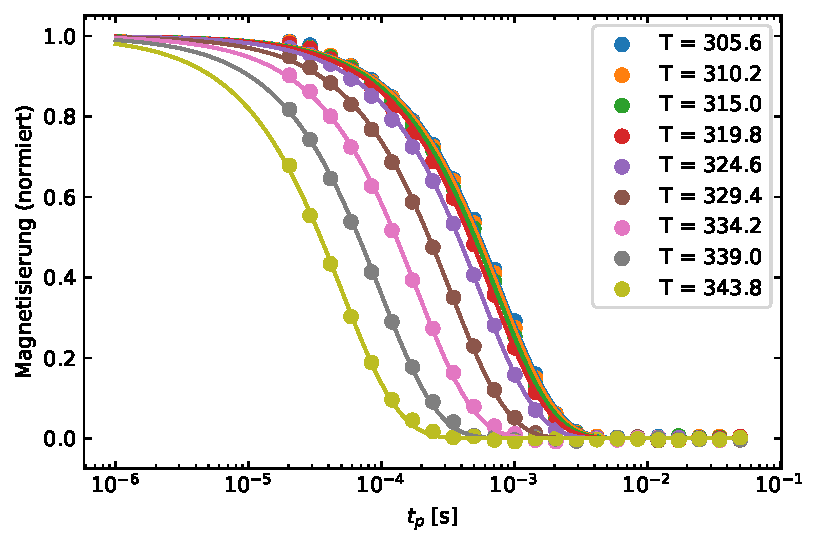
\includegraphics[width=.8\textwidth]{graphics/plot/t2_roh3.pdf}
	\end{center}
	\caption{Kurven des transversalen Magnetisierungszerfalls zur Bestimmung von $T_2$, aufgenommen am OBI-Spektrometer mit $\omega_{L, \text{OBI}} = 2\pi \cdot \SI{97.1722}{MHz}$. Linien stellen Kohlrausch-Fits an die Datenpunkte dar. Die Daten wurden auf $M_{T_2}(0) = 1$ und $M_{T_2}(\infty) = 0$ der Fits normiert.} \label{fig:res:T_2_roh}
\end{figure}
An diese wurden Fit-Funktionen nach \eqref{eqn:theo:T_2_fit} angelegt, welche als Linien dargestellt sind. Es lässt sich mit den Fits eine gute Übereinstimmung zu den Daten erzielen. Auch hier lässt sich erkennen, dass $T_2$ bei Temperaturen bis etwa $\SI{320}{\kelvin}$ nahezu konstant verbleibt und zu hoheren Temperaturen kleiner wird.

Abbildung \ref{fig:res:T_2} zeigt eine Übersicht über die aufgenommen $T_2$-Werte mit den zugehörigen $\beta$ der Fits. Unter $\SI{320}{\kelvin}$ verbleiben erstere im niedrigen Millisekunden-Bereich, ehe sie deutlich kürzer werden und sich bei etwa $\SI{360}{\kelvin}$ ein Minimum zeigt. Die Werte des Bruker-Spektrometers sind hiermit in guter Übereinstimmung, wobei wiederum festzuhalten ist, dass die Messunsicherheiten geringer sind. Ein zweites Minimum zeigt sich bei etwa $\SI{400}{\kelvin}$, dessen Wert sich, ebenso wie der erste, im zweistelligen Mikrosekunden-Bereich befindet. Zwischen $\SI{400}{\kelvin}$ und $\SI{410}{\kelvin}$ ist zu erkennen, dass -- wohl durch die Kürze von $T_2$ bei diesen Temperaturen -- deutlich größere Unsicherheiten als im Rest der Messreihe vorliegen, wo sie in guter Näherung vernachlässigbar sind.

Aus diesem Grund wurden hier zusätzliche Fits mit einem Konstanten $\beta = 1$ angefertigt, die in der Abbildung durch Sterne symbolisiert sind. Es ist zu erkennen, dass die so bestimmten $T_2$-Werte deutlich geringere Unsicherheiten zeigen, aber dem gleichen Verlauf folgen. Sie scheinen jedoch bei etwas kürzeren Werten zu liegen; der Quotient der Werte mit ihrem mit freiem $\beta$ bestimmten Gegenpart überschreitet den Wert 2 nicht.

Auch die $\beta$-Werte zeigen bei höheren Temperaturen deutlich größere Unsicherheiten, hier allerdings schon zwischen $\SI{390}{\kelvin}$ und $\SI{425}{\kelvin}$. Sie scheinen zwischen $\SI{1}{}$ und $\SI{2}{}$ zu liegen. Bei tieferen Temperaturen klärt sich das Bild etwas: Während die Daten des OBI-Spektrometers bei Temperaturen bis $\SI{350}{\kelvin}$ ein $\beta$ zwischen $\SI{1}{}$ und $\SI{1.5}{}$ suggerieren, zeigen die Daten des Bruker-Spektrometers ein $\beta$ um $\SI{1}{}$ -- mit geringerer Unsicherheit. Bei nochmals tieferen Temperaturen scheint $\beta$ konsistent bei rund $\SI{1}{}$ zu liegen.

\begin{figure}
	\begin{center}
		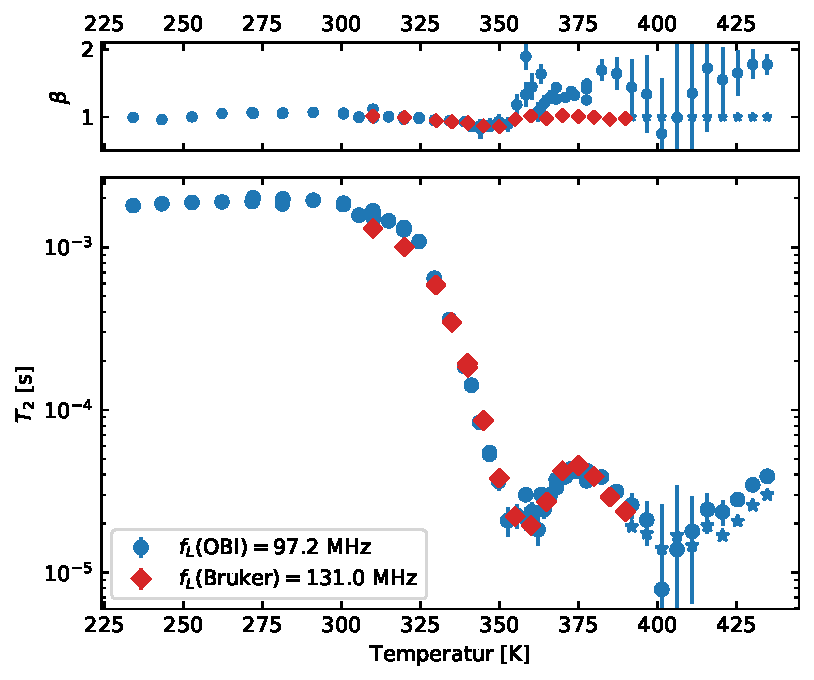
\includegraphics[width=.9\textwidth]{graphics/plot/t2.pdf}
	\end{center}
	\caption{$T_2$ und $\beta$ aus Fits nach Gleichung \eqref{eqn:theo:T_2_fit}. Blaue und rote Symbole zeigen die am OBI- bzw. Bruker-Spektrometer aufgenommen Daten. Bei Temperaturen über $\SI{390}{\kelvin}$ wurden zusätzlich Fits mit einem konstanten $\beta = \SI{1}{}$ erstellt -- diese Werte wurden mit Sternen anstatt Punkten symbolisiert.} \label{fig:res:T_2}
\end{figure}



\section{Untersuchung zur Dynamik von CRN} \label{section:res:F_2}

Mit der Absicht, einen möglichen Betaprozess zu identifizieren, wurden $F_2$-Messungen (siehe Kapitel \ref{section:theo:pulsfolgen}) und pulslängenabhängige Spektren aufgenommen; die verwendeten Methoden und Ergebnisse sollen im Folgenden vorgestellt werden

\subsection{Stimulierte Echos} \label{section:res:stimechos}

Es wurden am OBI-Spektrometer bei $\omega_{L, \text{OBI}} = 2\pi \cdot \SI{97.1722}{MHz}$ $F_2$-Messungen, also stimulierte Echos, über eine Reihe von Temperaturen von $\SI{230}{\kelvin}$ bis $\SI{310}{\kelvin}$ und Evolutionszeiten von $t_p = \SI{50}{\micro s}$ bis $t_p = \SI{1000}{\micro s}$ durchgeführt. Es wurde eine Drei-Puls-Folge verwendet und so sowohl Cos-Cos- als auch Sin-Sin-Korrelationen gemessen.

Bei Evolutionszeiten unter $t_p = \SI{1000}{\micro s}$ und Temperaturen unter $\SI{300}{\kelvin}$ waren die aufgenommenen Daten schwerlich oder gar nicht von $T_1$-Kurven zu unterscheiden, die bei gleicher Temperatur aufgenommen wurden. Es ist möglich, dass mit deutlich mehr Auswertungsaufwand auch hier Ergebnisse erzielt werden könnten; die vorliegende Auswertung soll sich jedoch mit den Temperaturen $\SI{300}{\kelvin}$ und $\SI{310}{\kelvin}$ mit $t_p = \SI{1000}{\micro s}$ befassen. Es wurde je eine Sin-Sin- und Cos-Cos-Messung bei $\SI{300}{\kelvin}$ und $\SI{310}{\kelvin}$ durchgeführt; diese Messreihe wurde als MR1 bezeichnet. Je eine weitere Sin-Sin- und Cos-Cos-Messung wurde bei $\SI{310}{\kelvin}$ aufgenommen. Diese als MR2 bezeichnete Messreihe unterscheidet sich von der ersten in der dreifachen Anzahl der Akkumulationen.

Einen Fit der Form \eqref{eqn:theo:F_2_fit} direkt an die Messwerte anzulegen erwies sich auch bei den höheren Temperaturen als schwierig, daher wurden mehrere Schritte für eine Auswertung durchgeführt. Formel \eqref{eqn:theo:F_2_fit} besteht aus einer Kombination von zwei Kohlrausch-Funktionen, von der jedoch bei der $F_2$-Messung insbesondere die Parameter $\tau_2$ und $\beta_{F_2}$ von Interesse sind. Um einen Fit zur Bestimmung dieser Werte möglich zu machen, soll die Daten von dem Einfluss der $T_1$-Relaxation, welche während auch während der Mischzeit auftritt, bereinigt werden. Dazu wird an die Daten zunächst folgende Funktion gefittet:
\begin{align}
	M_{F_2} (t_m) = M_0 \left[ \exp{ \left(- { \left( \frac{t_m}{\tau_2} \right) }^{\beta_{F_2}} \right)} \right] + M_\text{off} \label{eqn:res:F_2_fit}
\end{align}
Dieser Fit stellt die blaue Kurve in der oberen Hälfte von Abbildung \ref{fig:res:F_2_fit} dar. Die gezeigten Daten entstammen der Messreihe MR2 und wurden am OBI-Spektrometer mit $\omega_{L, \text{OBI}} = 2\pi \cdot \SI{97.1722}{MHz}$ bei einer Temperatur von $\SI{310}{\kelvin}$ und einer Evolutionszeit von $t_p = \SI{1000}{\micro s}$ mit einer Pulsfolge zur Bestimmung der Cos-Cos-Korrelation aufgenommen.
\begin{figure}
	\centering
	\begin{subfigure}{\textwidth}
		\centering
		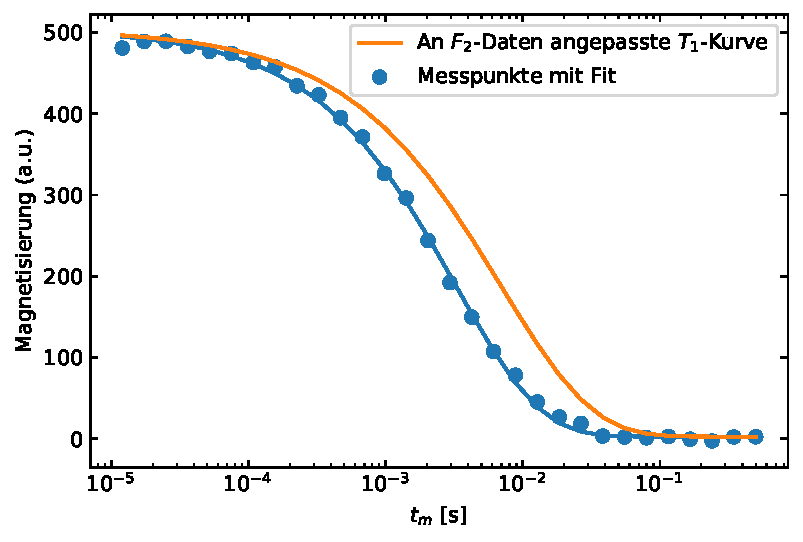
\includegraphics[width=0.8\textwidth]{graphics/plot/f2_310.pdf}
		% \label{fig:res:F_2_tieftemp}
	\end{subfigure} \\
	\begin{subfigure}{\textwidth}
		\centering
		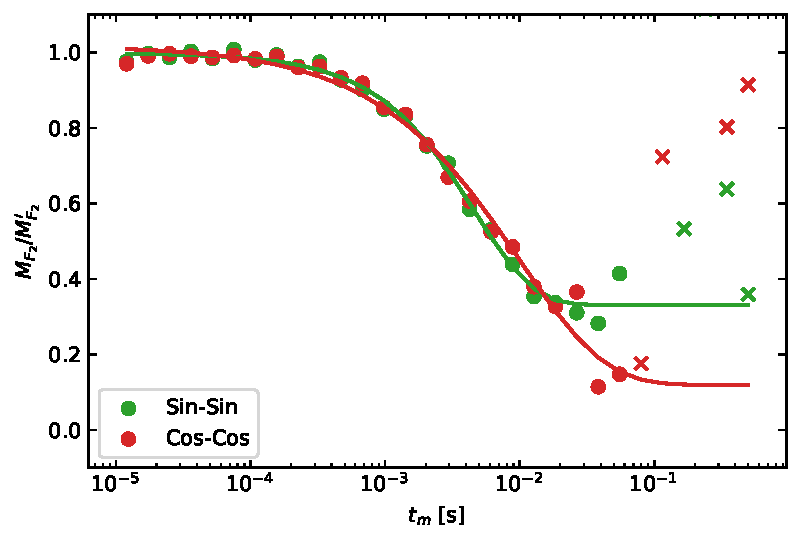
\includegraphics[width=0.8\textwidth]{graphics/plot/f2_fit3.pdf}
		% \label{fig:res:F_2_fit}
	\end{subfigure}
	\caption{Oben: $F_2$-Cos-Cos-Messungen mit $t_p = \SI{1000}{\micro s}$ am OBI-Spektrometer bei $\SI{310}{\kelvin}$ aus der Messreihe MR2. Die blaue Linie zeigt einen Fit an die Daten nach Gleichung \eqref{eqn:res:F_2_fit}, die orangene Linie die angepasste Funktion \eqref{eqn:res:F_2_angp}. Unten: Die Daten nach Gleichungen \eqref{eqn:res:F_2_fit} und \eqref{eqn:res:F_2_angp} durcheinander geteilt. An die entstandenden Daten wurden Kohlrausch-Fits (dargestellt als Linien) angelegt, um Zeitkonstanten zu gewinnen. Stark streuende Werte bei $t_m > \SI{60}{ms}$ wurden nicht in die Fits mit einbezogen und sind als Kreuze dargestellt. Die roten Daten korrespondieren zu den Daten der oberen Grafik; die grünen Daten sind unter den gleichen Umständen aufgenommene Sin-Sin-Messungen.}
	\label{fig:res:F_2_fit}
	\label{fig:res:F_2_T_1}
\end{figure}

Die Werte $\tau_2$ und $\beta_{F_2}$ wurden dann durch $T_1$ und $\beta_{T_1}$ einer $T_1$-Messung gleicher Temperatur ersetzt:
\begin{align}
	M_{F_2}' (t_m) = M_0 \left[ \exp{ \left(- { \left( \frac{t_m}{T_1} \right) }^{\beta_{T_1}} \right)} \right] + M_\text{off} \label{eqn:res:F_2_angp}
\end{align}
Das Resultat ist als orangene Kurve in der gleichen Abbildung gezeigt. Dieses Vorgehen macht es möglich, die $T_1$-Kurve an die $F_2$-Daten anzupassen. Die orangene Kurve symbolisiert, welchen Einfluss $T_1$ allein hat -- von Interesse sind alle weiteren Einflüsse, die zu einem Abfall der Magnetisierung führen. Daher wurden nun die Daten durch die angepasste $T_1$-Kurve geteilt, um den entsprechenden $T_1$-Anteil zu eliminieren. Das Resultat ist in Abbildung \ref{fig:res:F_2_T_1} unten gezeigt; dargestellt sind die Ergebnisse für die Cos-Cos-Messung (welcher die Daten der Grafik in der oberen Hälfte entstammen) und die Sin-Sin-Messung der Messreihe MR2.

An die so gewonnenen Daten kann wiederum ein Kohlrausch-Fit angelegt werden, um über den beschriebenen Umweg zu einer Funktion ähnlich der aus Formel \eqref{eqn:theo:F_2_fit} zu gelangen. Da die Quotienten bei Mischzeiten von über $\SI{60}{\milli s}$ stark streuen -- hier liegen beide Werte nahe 0 -- wurden sie aus dem Fit ausgeschlossen, um das Ergebnis nicht zu beeinträchtigen. Dies wurde in der Abbildung \ref{fig:res:F_2_T_1} durch die Verwendung von Kreuzen anstatt von Punkten symbolisiert.

Die gewonnenen Zeitkonstanten und $\beta$ der Kohlrausch-Fits an die Quotienten finden sich für beide Messreihen in Tabelle \ref{tab:res:F_2} und später in Abbildung \ref{fig:res:dynvgl}.
\begin{table}
	\centering
	\begin{tabular}{lllll}
		\hline
		Temperatur & Sin-Sin $\tau$ & Sin-Sin $\beta$ & Cos-Cos $\tau$ & Cos-Cos $\beta$ \\ \hline
		$\SI{300}{\kelvin}$ (MR1) & $\SI{5.26 (94)}{\milli s}$ & $\SI{0.95 (18)}{}$ & $\SI{3.68 (63)}{\milli s}$ & $\SI{1.30 (34)}{}$ \\
		$\SI{310}{\kelvin}$ (MR1) & $\SI{3.27 (122)}{\milli s}$ & $\SI{1.12 (56)}{}$ & $\SI{9.95 (432)}{\milli s}$ & $\SI{0.74 (21)}{}$ \\
		$\SI{310}{\kelvin}$ (MR2) & $\SI{4.23 (37)}{\milli s}$ & $\SI{1.01 (10)}{}$ & $\SI{3.28 (7)}{\milli s}$ & $\SI{0.71 (1)}{}$ \\
		 \hline
	\end{tabular}
	\caption{Resultate der $F_2$-Messungen. Sin-Sin und Cos-Cos beziehen sich auf die jeweils verwendete Pulsfolge, $\tau$ und $\beta$ sind die mit den Fits bestimmten Parameter der Zeitkonstante und der Streckung der Exponentialfunktion. \label{tab:res:F_2}}
\end{table}

Es ist zu erkennen, dass die Größen zwischen den zwei Messreihen teils mehr schwanken als zwischen zwei Temperaturen oder im Vergleich zwischen Sin-Sin- und Cos-Cos-Pulsfolgen. Da die Unsicherheiten zudem in Fällen beinahe $\SI{50}{\percent}$ erreichen, müssen diese Ergebnisse mit Vorsicht betrachtet werden. Die Werte der Messreihe MR2 sind, wohl aufgrund her höheren Anzahl von Akkumulationen, mit geringeren Unsicherheiten behaftet.



\subsection{Pulslängenabhängige Spektren} \label{section:res:spekdyn}

Eine weitere Untersuchung zu möglicher Dynamik wurde an der sich ändernden Linienform von pulslängenabhängigen Spektren durchgeführt. Während hier nur auf die Bestimmung von Zeitkonstanten eingegangen werden soll, werden die Details von der Linienform von CRN-Spektren im späteren Abschnitt \ref{section:res:spektren} diskutiert.

Es wurde beobachtet, dass Spektren, die mit einem Hahn-Echo mit unterschiedlicher Evolutionszeit $t_p$ aufgenommen wurden, eine unterschiedliche Linienform zeigen. Die Halbwertsbreiten der normierten Spektren sind also evolutionszeitabhängig, und das bei verschiedenen Temperaturen in verschiedenen Maßen. Dies lässt sich in Abbildung \ref{fig:res:spekdyn_305K} erkennen, wo normierte, pulslängenabhängige Spektren für die Temperaturen $\SI{305}{\kelvin}$ oben bzw. $\SI{325}{\kelvin}$ unten gezeigt sind. Die Daten wurden am OBI-Spektrometer mit $\omega_{L, \text{OBI}} = 2\pi \cdot \SI{97.1722}{MHz}$ aufgenommen und mit Gaußfunktion mit einer Breite von $\SI{500}{Hz}$ apodisiert. Diese Faltung sorgt für eine Verbreiterung der Spektren, welche zwar die Auflösung, aber auch das Rauschen verringert.
\begin{figure}
	\centering
	\begin{subfigure}{\textwidth}
		\centering
		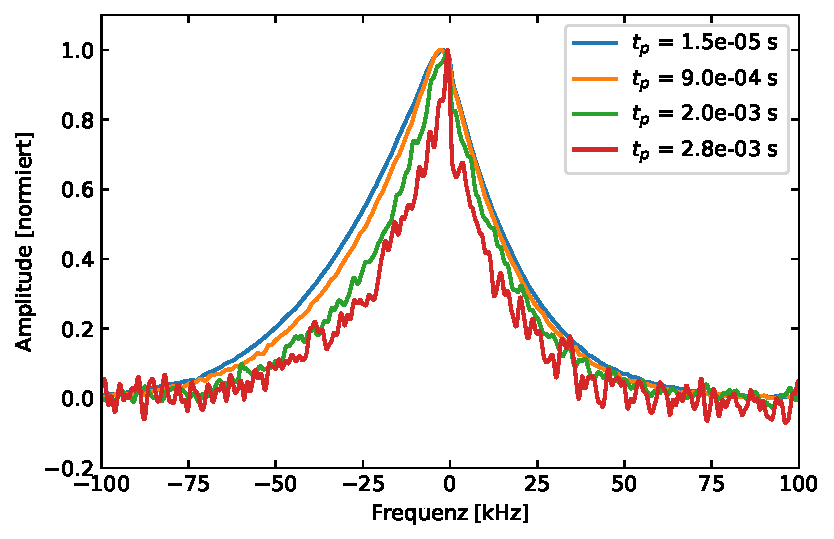
\includegraphics[width=.9\textwidth]{graphics/plot/spekdyn_305K2.pdf}
	\end{subfigure} \\
	\begin{subfigure}{\textwidth}
		\centering
		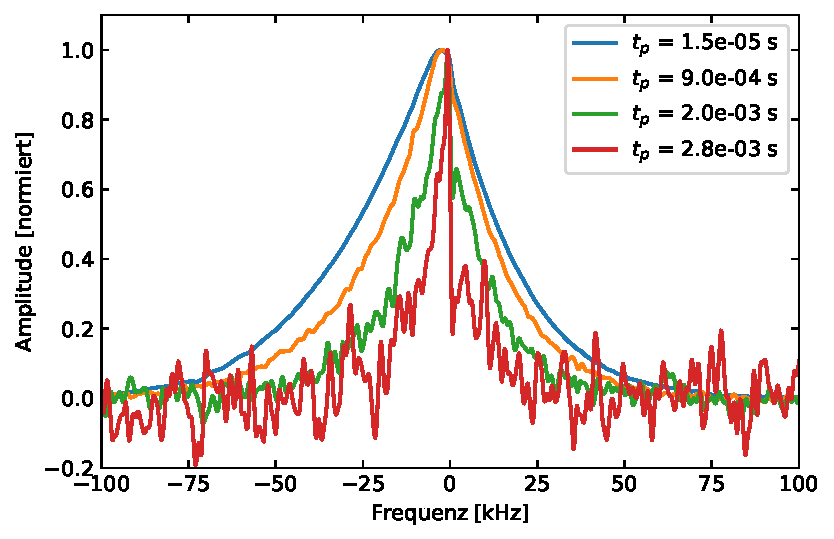
\includegraphics[width=.9\textwidth]{graphics/plot/spekdyn_325K2.pdf}
	\end{subfigure}
	\caption{Änderung der Linienform der mit einem Hahn-Echo aufgenommenen Spektren bei $\SI{305}{\kelvin}$ (oben) und bei $\SI{325}{\kelvin}$ (unten) in Abhängigkeit der Evolutionszeit $t_p$. Die Daten wurden am OBI-Spektrometer mit $\omega_{L, \text{OBI}} = 2\pi \cdot \SI{97.1722}{MHz}$ aufgenommen und auf ihr Maximum normiert.}
	\label{fig:res:spekdyn_305K}
	\label{fig:res:spekdyn_325K}
\end{figure}

Zur Untersuchung der Evo\-lu\-tions\-zeit-Ab\-häng\-ig\-keit wurde für jede Temperatur die Halbwertsbreite -- als Maß für die Linienform -- gegen die Evolutionszeit $t_p$ aufgetragen. An diese Daten wurden Kohlrausch-Fits angelegt, die als durchgezogene Linien, zusammen mit dem Daten, in Abbildung \ref{fig:res:spekdyn_fits} zu sehen sind. Alle Spektren wurden am OBI-Spektrometer aufgenommen. Da die Spektren bei zunehmenden Pulslängen ein immer schlechteres Sig\-nal-Rausch-Ver\-hält\-nis aufweisen -- beispielhaft zu erkennen in der unteren Hälfte der Abbildung \ref{fig:res:spekdyn_325K} für $t_p = \SI{2.7}{\milli s}$ --, wurden die verwendeten Evolutionszeiten auf $\SI{2}{\milli s}$ begrenzt. 
\begin{figure}
	\begin{center}
		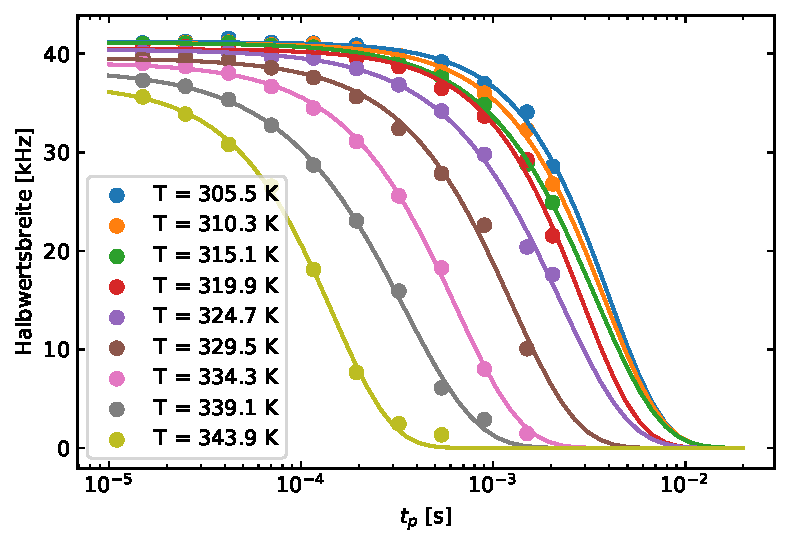
\includegraphics[width=.9\textwidth]{graphics/plot/spekdyn_fits2.pdf}
	\end{center}
	\caption{Halbwertsbreiten der Spektren in Abhängigkeit von $t_p$. An diese Daten wurden Kohlrausch-Fits angelegt, dargestellt als durchgezogene Linien.} \label{fig:res:spekdyn_fits}
\end{figure}

Es wurde eine weitere, ähnliche Auswertung durchgeführt, wobei anstatt der Halbwertsbreite die Amplitude bei einer bestimmten Frequenz (beispielsweise bei $\SI{-15}{\kilo Hz}$) als Variable genommen wurde. Die Ergebnisse glichen der der Halbwertsbreiten-Betrachtung, waren aber durchgehend mit Unsicherheiten in Größenordnung der eigentlichen Werte behaftet. Dies lässt sich durch die stark verrauschten Spektren bei hohen Evolutionszeiten erklären, die zu stark schwankenden Amplituden führen, welche wiederum einen guten Fit der Daten schwierig gestalten. Es ist die Untersuchung der Halbwertsbreiten dieser Methode vorzuziehen.



\subsection{Auswertung der experimentell bestimmten Zeitkonstanten} \label{section:res:dynausw}

Werden die bestimmten Zeitkonstanten der $T_1$-, $T_2$-, $F_2$- und $t_p$-abhängigen Spek\-trums-Mess\-un\-gen zusammen aufgetragen, ergibt sich das in Abbildung \ref{fig:res:dynvgl} gezeigt Bild.
\begin{figure}
	\begin{center}
		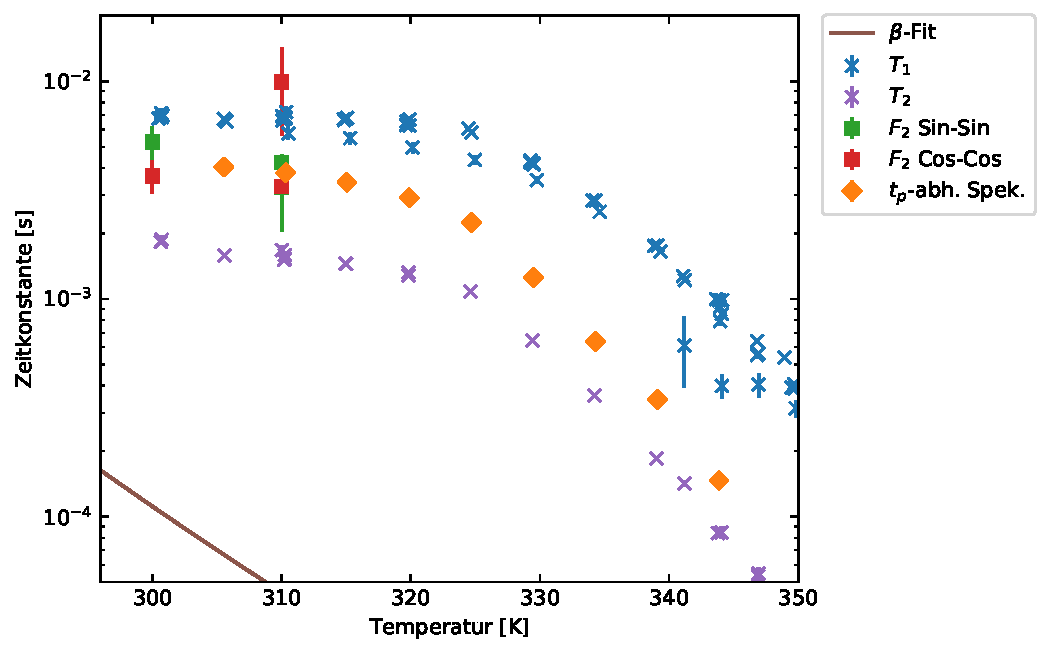
\includegraphics[width=.9\textwidth]{graphics/plot/dyn.pdf}
	\end{center}
	\caption{Vergleich der gewonnenen Zeitkonstanten.
	
	Die braune Linie entspricht der gestrichelten Linie aus Abbildung \ref{fig:einl:zuernpaper}, welche ein Fit an Zeitkonstanten eines Betaprozesses ist.} \label{fig:res:dynvgl}
\end{figure}
Alle bestimmten Zeitkonstanten liegen -- im Rahmen der Unsicherheiten -- zwischen den bestimmten $T_1$- und $T_2$-Werten. Diese Unsicherheiten sind bei fast allen Messungen, mit Ausnahme der $F_2$-Messungen, unter der verwendeten Symbolgröße und können vernachlässigt werden. Gründe für die höheren Unsicherheiten der $F_2$-Messungen könnten die mehrschrittige Auswertung und die verrauschten Signale bei hohen Evolutionszeiten sein.

Ab $\SI{320}{\kelvin}$ bis $\SI{330}{\kelvin}$ zeigen alle Zeitkonstanten einen Übergang zu kürzeren Zeiten, der wohl mit der höheren Bewegung der Atome in der Nähe der Glasübergangstemperatur von $T_g = \SI{333}{\kelvin}$ einhergeht. Dieser Effekt ist auch als Bewegungsverschmälerung in Spektren zu sehen (vgl. Abbildung \ref{fig:res:spek_fwhm}).

Die braune Linie stellt dabei einen Fit durch die in Abbildung \ref{fig:einl:zuernpaper} gezeigten, zum Betaprozess gehörenden Werte dar. Die Linie kann eine Abschätzung zu geben, in welcher Größenordnung der Prozess im untersuchten Temperaturbereich liegt, sollte sich der angedeutete Trend im Arrhenius-Diagramm \ref{fig:einl:zuernpaper} linear fortsetzen. Wie zu erkennen, befindet sich keine der bestimmten Zeitkonstanten in der entsprechenden Größenordnung. Dies bedeutet möglicherweise, dass der Prozess mit den hier verwendeten Methoden nicht detektiert werden kann -- ein zu geringer Einfluss könnte der Grund sein. Weitere Untersuchungen sind nötig, um diese Frage abschließend klären zu können.



\section{Linienform von experimentellen und simulierten CRN-Spektren} \label{section:res:spektren}

Das zweite Ziel dieser Arbeit ist die Untersuchung der Linienform von CRN-Spek\-tren. Bei der Auswertung von Spektren wurde eine zunächst ungewöhnlich erscheinende Verbreiterung derselben in einem Temperaturbereich beobachtet, wo, aufgrund von Bewegungsverschmälerung, eher kleinere Halbwertsbreiten zu erwarten wären. Zur Untersuchung der Gegebenheiten wurden, neben einer Vielzahl von experimenteller Spektren, Computer-Simulationen angefertigt und versucht, eine theoretische Erklärung der Daten zu bieten.

\begin{figure}
	\begin{center}
		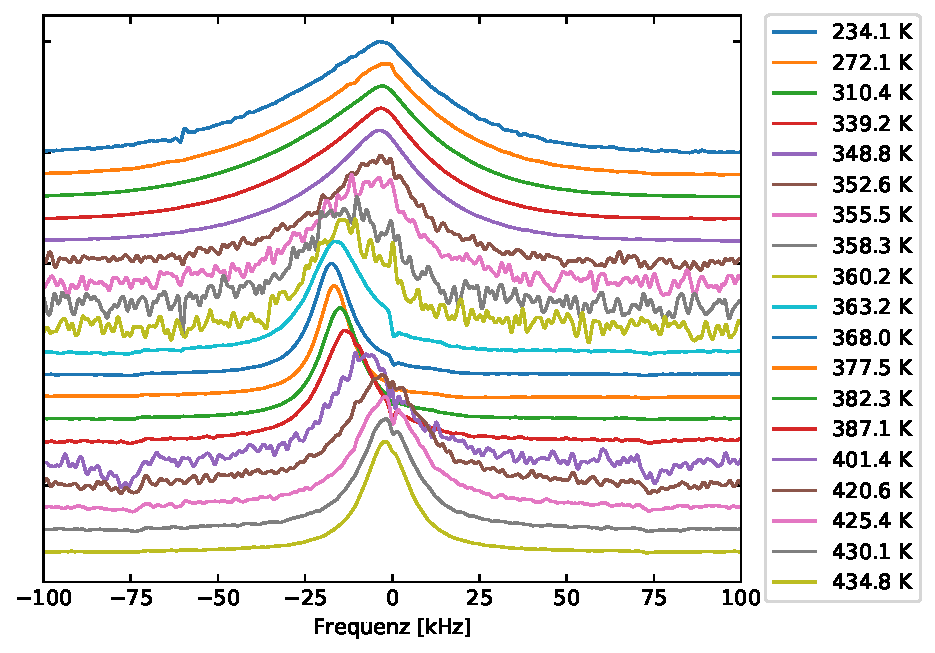
\includegraphics[width=\textwidth]{graphics/plot/spek_lineshape.pdf}
	\end{center}
	\caption{Vergleich der Linienform von am OBI-Spektrometer aufgenommen Spektren.} \label{fig:res:spek_linienform}
\end{figure}
Um eine Übersicht zu schaffen, werden zuerst die Linienformen der Spektren aus den verschiedenen Quellen in Abhängigkeit der Temperatur präsentiert. Abbildung \ref{fig:res:spek_linienform} zeigt die am OBI-Spektrometer aufgenommenen Spektren; die Temperaturen reichen von etwa $\SI{234}{\kelvin}$ bis etwa $\SI{435}{\kelvin}$. Sie wurden mit einem Hahn-Echo mit einer Evolutionszeit von $t_p = \SI{15}{\micro s}$ aufgenommen und mit $\SI{500}{Hz}$ apodisiert. Es wurden je $\SI{8192}{}$ Datenpunkte mit einer Frequenz von $\SI{2}{MHz}$ erstellt. Die Spektren wurden in mehreren Messreihen aufgenommen und stellen eine repräsentative Auswahl dar, die es erlaubt, den Verlauf der Linienform nachzuvollziehen, ohne zu stark an Übersicht zu verlieren.

Bei tiefen Temperaturen ist eine Form zu beobachten, die der des Czjzek-Spektrums aus Kapitel (***) ähnelt. Diese hält sich über weite Temperaturen, von etwa $\SI{235}{\kelvin}$ bis etwa $\SI{350}{\kelvin}$, fast unverändert. Bei steigenden Temperaturen ändert sich die Linienform, sie nimmt die einer Lorentz-Funktion
\begin{align}
	L(f) = \frac{1}{\pi \gamma} \cdot \frac{\gamma^2}{\gamma^2 + (f - f_0)^2} \label{eqn:res:lorentz}
\end{align}
an, während die Spektren gleichzeitig schmaler werden und sich der Schwerpunkt zu niedrigeren Frequenzen verschiebt. Diese Bewegung findet ein Ende bei etwa $\SI{367}{\kelvin}$: Zu höheren Temperaturen verbreitern sich die Spektren wieder, ehe sie ab $\SI{410}{\kelvin}$ wieder schmaler werden. Der Schwerpunkt verschiebt sich ab 375K wieder gegen $\SI{0}{Hz}$, wo er ab 400K verweilt. Die Linienform ändert sich nicht mehr.

Es ist auffällig, dass die Qualität der Spektren stark mit der Temperatur schwankt. Zwischen $\SI{235}{\kelvin}$ und $\SI{350}{\kelvin}$, $\SI{363}{\kelvin}$ und $\SI{387}{\kelvin}$, sowie zwischen $\SI{430}{\kelvin}$ und $\SI{435}{\kelvin}$ weisen die Spektren vergleichsweise geringes Rauschen und somit eine glattere Form auf. Die abschnittweise höheren Schwankungen lassen sich durch $T_2$-Minima (siehe Abbildung \ref{fig:res:T_2}) bei den entsprechenden Temperaturen erklären -- diese sorgen für einen schnellen Abfall des Signals und entsprechend verrauschte Spektren.

\begin{figure}
	\begin{center}
		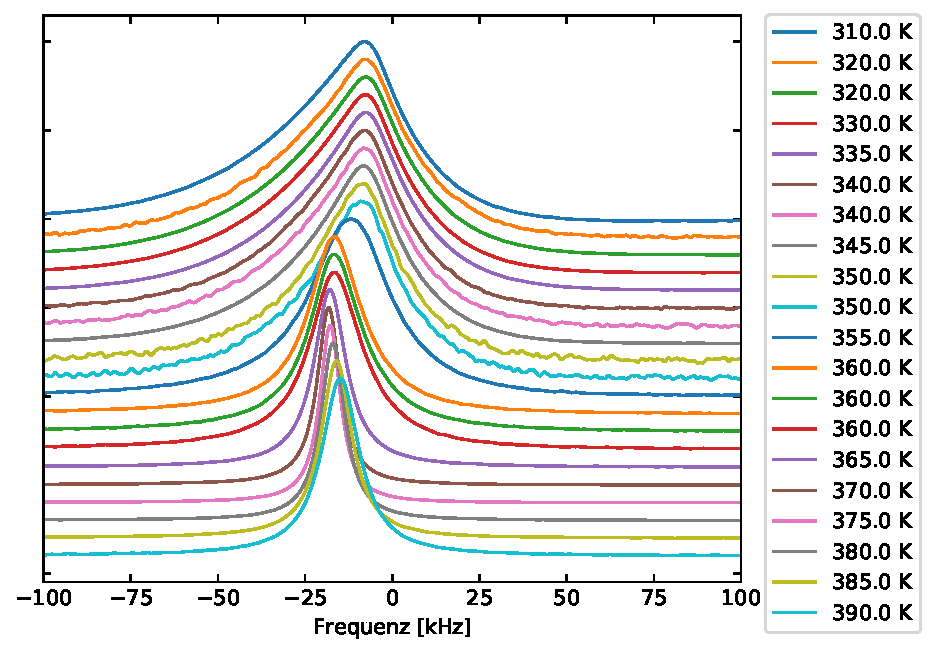
\includegraphics[width=\textwidth]{graphics/plot/bruker_lineshape.pdf}
	\end{center}
	\caption{Vergleich der Linienform von am Bruker-Spektrometer aufgenommen Spektren.} \label{fig:res:bruker_linienform}
\end{figure}
Die am Bruker-Spektrometer aufgenommenen Spektren decken einen Temperaturbereich von $\SI{310}{\kelvin}$ bis $\SI{390}{\kelvin}$ ab und wurden ebenfalls mit einem Hahn-Echo mit einer Evolutionszeit von $\SI{15}{\micro s}$ erstellt und mit $\SI{500}{Hz}$ apodisiert. Hier wurden je $\SI{4096}{}$ Datenpunkte mit einer Frequenz von $\SI{0.5}{MHz}$ aufgenommen. Da mit diesem Spektrometer weitaus weniger Spektren erstellt wurden als mit dem OBI-Spektrometer, können in Abbildung \ref{fig:res:bruker_linienform} alle erstellten Spektren präsentiert werden.

Der Verlauf der Linienform gleicht der beschriebenen in dem entsprechenden Temperaturbereich gut. Es ist das geringe Rauschen der Spektren zu beachten, das, wie auch insbesondere die $T_2$-Daten, ein Beleg für hohe Datenqualität des Bruker-Spektrometers in diesem Kontext ist.

Als Ergänzung zu den experimentellen Daten wurden Spektren simuliert. Dazu wurde die in Kapitel (***) vorgestellte Simulations-Software verwendet. Es wurden FIDs mit $\SI{4096}{}$ Datenpunkten mit einem Abstand von je $\SI{0.5}{\micro s}$, was einer Frequenz von $\SI{2}{MHz}$ entspricht, aufgenommen. Um einen Mittelwert zu bilden, wurden, je nach Spektrum, zwischen $10^{7}$ und $10^{9}$ einzelne Trajektorien gemittelt. Als Modell wurde ein isotroper Zufallssprung gewählt, welcher eine Czjzek-Verteilung als Ausgangspunkt hat; dieses war der simulierten Quadrupol-Wechselwirkung zweiter Ordnung ausgesetzt. Zur Bestimmung der Lebensdauer eines bestimmten Zustandes wurde eine Exponentialverteilung genutzt, deren Parameter, die Lebenszeit, eine Verknüpfung mit Temperaturen ermöglicht. Es wurde eine Vogel-Fulcher-Funktion für die Lebenszeit mit den Parametern für CRN aus \cite{PIMENOV199793} verwendet. Zur besseren Vergleichbarkeit werden im Folgenden die Spektren mit den so berechneten Temperaturen anstatt mit den Lebenszeiten referenziert. Die resultierenden Spektren sind in Abbildung \ref{fig:res:sim_linienform} zu sehen. Da die Breite der Spektren in der Simulation mit nur einem frei wählbaren Parameter bestimmt wird, wurde sie durch das Vergleichen der Form bei tiefen Temperaturen normiert.
\begin{figure}
	\begin{center}
		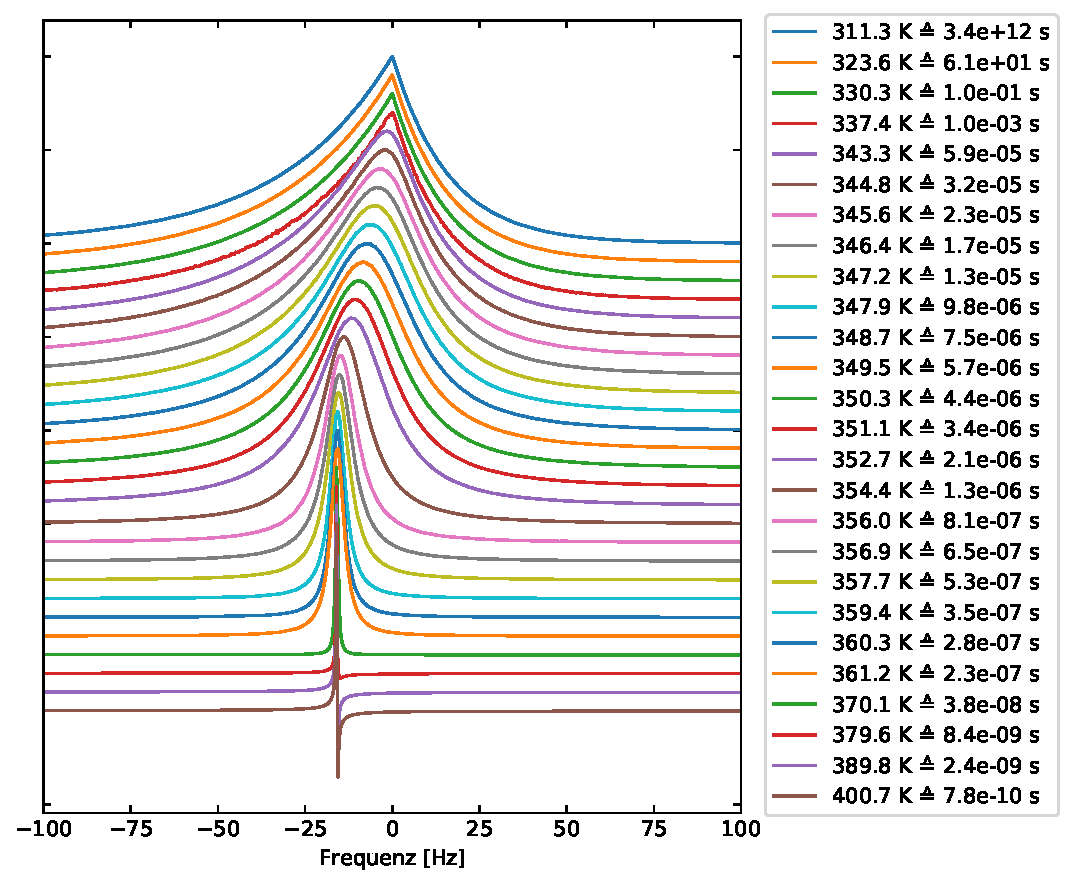
\includegraphics[width=\textwidth]{graphics/plot/sim_lineshape.pdf}
	\end{center}
	\caption{Vergleich der Linienform von mit Simulationen erstellte Spektren. Die angegebenen Temperaturen wurden mithilfe von den in Kapitel \ref{section:res:theorie} beschriebenen $\tau_c$ aus den verwendeten $\tau$ bestimmt.} \label{fig:res:sim_linienform}
\end{figure}

Bei tiefen Temperaturen gleichen die simulierten Spektren den experimentellen; dies wurde schon in \cite{joachim_master} gefunden. Auch ist der Übergang zur Lorentz-Form, verbunden mit der Verschiebung des Schwerpunkts und Verschmälerung der Spektren bei etwa der gleichen Temperatur von $\SI{350}{\kelvin}$ zu beobachten. Im Gegensatz zu den experimentellen Spektren werden die simulierten Spektren mit steigender Temperatur jedoch immer schmaler und ändern den Schwerpunkt nicht mehr.


Um eine quantitative Behandlung der Spektren zu ermöglichen, wurden zwei Messgrößen verwendet: Die Halbwertsbreite (also die Breite auf der Höhe der Hälfte des Maximums) und der Schwerpunkt der Spektren. Um bei den stark verrauschten Spektren des OBI-Spektrometers zwischen $\SI{350}{\kelvin}$ und $\SI{360}{\kelvin}$ und zwischen $\SI{390}{\kelvin}$ und $\SI{430}{\kelvin}$ gut vergleichbare Werte zu erhalten, wurde ein Lorentz-Fit nach Gleichung \eqref{eqn:res:lorentz} mit einer least-squares-Methode an die Spektren angelegt. So entspricht $2 \gamma$ der Halbwertsbreite und das Maximum $f_0$, aufgrund der Symmetrie der Funktion, dem Schwerpunkt. Die so gewonnenen Halbwertsbreiten sind in Abbildung \ref{fig:res:spek_fwhm} zu sehen.
\begin{figure}
	\begin{center}
		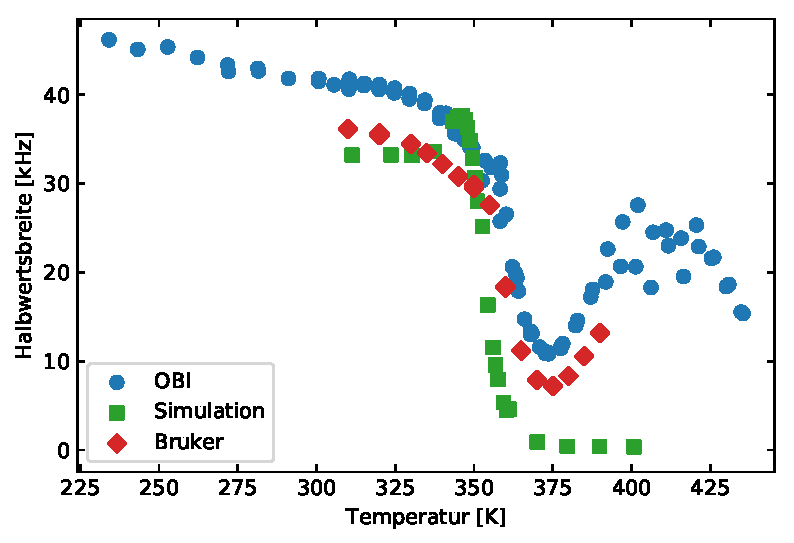
\includegraphics[width=.9\textwidth]{graphics/plot/fwhm.pdf}
	\end{center}
	\caption{Die Halbwertsbreite der Spektren. Blaue und rote Symbole kennzeichnen am OBI- bzw. Bruker-Spektrometer aufgenommene Spektren, grüne Symbole stammen von simulierten Spektren. Der auffälligste Unterschied zwischen experimentellen und simulierten Spektren ist das zusätzliche Maximum bei hohen Temperaturen bzw. dessen Fehlen.} \label{fig:res:spek_fwhm}
\end{figure}

Es ist zu erkennen, dass die Werte der Halbwertsbreite etwa dem entsprechen, was nach einer Betrachtung der Spektren zu erwarten wäre: Von einem Spektrum mit etwa $\SI{40}{kHz}$ Breite bei niedrigen Temperaturen gehen die Werte zu einem Minimum von etwa $\SI{10}{kHz}$ bei etwa $\SI{375}{\kelvin}$ über, um nach einem lokalen Maximum von rund $\SI{20}{kHz}$ bei etwa $\SI{400}{\kelvin}$ erneut abzufallen.

Diesem Verlauf der am OBI-Spektrometer aufgenommenen Spektren folgen auch die Halbwertsbreiten der am Bruker-Spektrometer produzierten Daten. Letztere liegen allerdings konstant bei niedrigeren Werten. Das Verhältnis entspricht aber auch nicht durchgehend dem Verhältnis $4:3$, was die entsprechend unterschiedlichen Larmorfrequenzen suggerieren würden; es liegt bei tiefen Temperaturen etwas niedriger und bei höheren Temperaturen etwas höher. So ist im Bereich zwischen $\SI{310}{\kelvin}$ und $\SI{350}{\kelvin}$ ein Verhältnis von etwa $\SI{1.15}{}:1$ zu finden, zwischen $\SI{360}{\kelvin}$ und $\SI{390}{\kelvin}$ ein Verhältnis von $\SI{1.45}{}:1$ bis $\SI{1.55}{}:1$. Messungen an einem $\SI{600}{MHz}$-Spektrometer wären hilfreich, um fundiertere Aussagen über Larmorfrequenz-abhängige Effekte treffen zu können.

Der Verlauf der Halbwertsbreiten der simulierten Spektren unterscheidet sich deutlich von dem der experimentellen Spektren. Während der grobe Verlauf übereinstimmt -- von breiten Spektren bei tiefen Temperaturen zu schmalen Spektren bei höheren Temperaturen -- sind bei genauerer Betrachtung starke Abweichungen zu sehen. Die simulierten Spektren werden zu höheren Temperaturen zunehmend schmaler und näheren sich einem Delta-Peak, während die Breiten der experimentellen Spektren ein weiteres Maximum aufweisen. Zudem ist ein Maximum der Halbwertsbreite der simulierten Spektren bei etwa $\SI{345}{\kelvin}$ zu beobachten, während die Halbwertsbreite der experimentellen Spektren einen fließenden Übergang der Breite von hohen zu tiefen Temperaturen zeigen.

Es sollte darauf aufmerksam gemacht werden, dass die Halbwertsbreite stark von der Form der Spitze beeinflusst wird, welche das Maximum und damit die Hälfte des Maximums bestimmt. Sind, wie bei den simulierten Spektren, extrem gut definierte Maxima zu sehen, drückt dies den Wert der Halbwertsbreiten im Vergleich zu den experimentellen Halbwertsbreiten nach unten. Dies erklärt den Abfall der Halbwertsbreiten der simulierten Spektren zu tieferen Temperaturen: Hier sind die scharfen Spitzen der Czjzek-Spektren gut ausgeprägt, sodass die Halbwertsbreite der Spektren beim Übergang zur abgerundeten Lorentz-Form ein Maximum durchläuft. Die experimentellen Spektren hingegen zeigen aufgrund von experimentellen Beschränkungen wie der Auflösung, und möglicherweise durch weitere Effekte, bei niedrigeren Temperaturen keine perfekte Spitze und daher auch keinen Peak in der Halbwertsbreite beim Übergang zur Lorentz-Form.

\par\bigskip

In Abbildung \ref{fig:res:spek_mean} sind die Schwerpunkte der Spektren aufgetragen. Diese wurden mit Hilfe von numerischer Integration nach der Simpsonregel bestimmt. Bei stark verrauschten Spektren, wo dieses Vorgehen wenig Erfolg verspricht -- es wird eher der Schwerpunkt der Schwankungen bestimmt als der des Signals --, wurden wieder Lorentz-Fits ausgenutzt, deren Parameter $f_0$ der Schwerpunkt ist.
\begin{figure}
	\begin{center}
		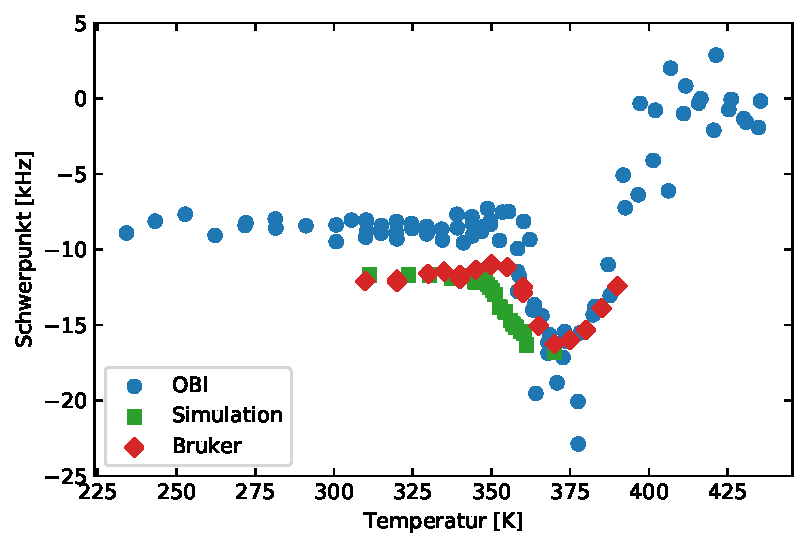
\includegraphics[width=.9\textwidth]{graphics/plot/mean.pdf} 
	\end{center}
	\caption{Die Halbwertsbreite der Spektren. Blaue und rote Symbole kennzeichnen am OBI- bzw. Bruker-Spektrometer aufgenommene Spektren, grüne Symbole stammen von simulierten Spektren. Während der Schwerpunkt der experimentellen Spektren zu hohen Temperaturen gegen $\SI{0}{\kilo Hz}$ geht, verbleibt der Schwerpunkt der simulierten Spektren bei etwa $\SI{-16}{\kilo Hz}$.} \label{fig:res:spek_mean}
\end{figure}

Allen drei Kurvenverläufen ist gleich, dass sie bei tieferen Temperaturen bis etwa $\SI{360}{\kelvin}$ einen konstanten Wert zeigen, ehe sich der Schwerpunkt zu niedrigeren Frequenzen von etwa $\SI{-16}{\kilo Hz}$ verschiebt, was mit dem Übergang von der Czjzek-Form des Spektrums zur Lorentz-Form einhergeht. Die spezifischen konstanten Werte der tieferen Temperaturen unterscheiden sich jedoch zwischen den Daten des OBI-Spektrometers mit einem Schwerpunkt von etwa $\SI{-8}{\kilo Hz}$ und den Daten des Bruker-Spektrometers und der Simulation mit einem Schwerpunkt von etwa $\SI{-12}{\kilo Hz}$. Auch in diesem Kontext könnten Messungen an Spektrometern mit unterschiedlichen Larmorfrequenzen helfen, um beispielsweise den Einfluss der chemischen Verschiebung auf die Position der Schwerpunkte zu untersuchen.

Ab etwa $\SI{375}{\kelvin}$ ist eine Bewegung des Schwerpunkts der experimentellen Spektren zum Nullpunkt zu erkennen, die die Spektren des OBI-Spektrometers aufgrund des größeren abgedeckten Temperaturbereichs auch erreichen. Die simulierten Spektren verbleiben jedoch bei dem Wert von $\SI{-16}{\kilo Hz}$, der bei $\SI{370}{\kelvin}$ erreicht wird.

Auch hier ist einschränkend zu sagen, dass die Werte der Schwerpunkte aufgrund von externen Faktoren instabil sind, mehr noch als die Halbwertsbreiten. Wie in Kapitel \ref{section:exp:weiterverarbeitung} erwähnt, wird eine Phasenanpassung des Real- und Imaginärteils durchgeführt, um ein maximales Signal zu garantieren und mögliche Schwankungen der Phase durch experimentelle Einflüsse auszugleichen. Allerding kann eine Abweichung von $\pm \SI{1}{\degree}$ vom Optimalwert unter den schlechtesten Umständen eine Verschiebung des Schwerpunkts um $\SI{1}{\kilo Hz}$ bewirken. Diese Empfindlichkeit gegenüber kleinen Änderungen bedeutet, dass Schwankungen der dargestellten Werte nicht auszuschließen sind; die groben Merkmale der Kurvenverläufe können aber leicht durch eine Betrachtung der Spektren bestätigt werden.




\section{Vergleich von CRN-Spektren mit theoretischen Überlegungen} \label{section:res:theorie}

Die experimentellen Ergebnisse sollen mit den theoretischen Überlegungen vergleichen werden. Dazu wurden die in Kapitel \ref{section:theo:qww} beschriebenen Funktionen für $T_1$, Halbwertsbreite und Schwerpunkt verwendet. Um eine Übereinstimmung zur Theorie feststellen zu können, müssen sich alle Datensätze mit dem gleichen Satz geteilter Parameter beschreiben lassen. Im Falle der Spektraldichte $J_\text{BPP}$ ist dies $C_Q$; für $J_\text{CC}$ und $J_\text{CD}$ sind $\alpha$ bzw. $\gamma$ zusätzliche Parameter.

Für den Parameter $\eta$ der Spektraldichten wurde $\eta^2 = 42 - 24 \sqrt{3} \approx \SI{0.43}{}$ \cite{caer} verwendet. Nach \cite{PIMENOV199793} wird für CRN für die Korrelationszeit $\tau_c$ ein Vogel-Fulcher-Gesetz
\begin{align}
	\tau_c = \tau_{co} \exp \left( \frac{D T_\text{VF}}{T-T_\text{VF}} \right)
\end{align}
mit dem strength index $D = \SI{3.5}{}$, der Vogel-Fulcher-Temperatur $T_\text{VF} = \SI{294}{K}$ und dem Frequenzfaktor $\tau_{co} = \SI{5.1e-14}{s}$ angenommen. Diese Werte wurden durch dielektrische Spektroskopie gewonnen.

Am $T_1$-Minimum nach Gleichung \eqref{eqn:bpp} gilt $\omega \tau_c \approx \SI{0.61}{}$ \cite[S. 629]{omegatau061}. Das $T_1$-Minimum kann in den OBI-Daten bei etwa $T_{T_1 \text{min}} = \SI{410}{K}$ gefunden werden; die Larmorfrequenz liegt bei $\omega_L = 2\pi \cdot \SI{97.1722}{MHz}$, was bedeutet, dass bei $T_{T_1 \text{min}}$ gilt $\tau_c \approx \sfrac{\SI{0.61}{}}{\omega_L} \approx \SI{1.0}{\nano s}$. Vergleicht man das Vogel-Fulcher-Gesetz mit diesem Punkt, lässt sich erkennen, dass eine gute Übereinstimmung vorliegt.

\begin{wrapfigure}{r}{0.5\textwidth}
	\vspace{-20pt}
	\begin{center}
		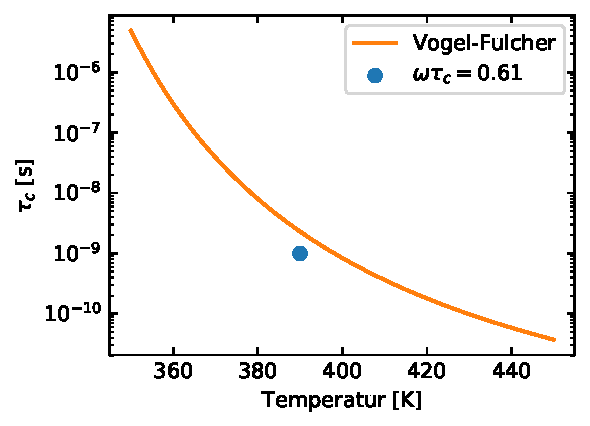
\includegraphics[width=0.49\textwidth]{graphics/plot/vftau.pdf}
	\end{center}
	\vspace{-20pt}
	\caption{Vergleich von Zeitkonstante aus $T_1$-Minimum, und Vogel-Fulcher-Gesetz für CRN mit Parametern nach \cite{PIMENOV199793} in orange und Parametern nach \cite{crn_augsburg} in grün. \label{fig:korrelationszeiten}}
\end{wrapfigure}
Ein Vergleich mit den Parametern $D = \SI{4.72}{}$, $T_\text{VF} = \SI{285}{K}$ und $\tau_{co} = \SI{1.15e-14}{s}$ nach \cite{crn_augsburg}, ebenfalls bestimmt durch dielektrische Spektroskopie, ist in den Abbildungen \ref{fig:korrelationszeiten} und \ref{fig:res:theorie_j} zu sehen. Während leichte Unterschiede zu erkennen sind, ändert sich das Gesamtbild wenig, weswegen sich diese Ausführungen auf den ersten Parametersatz beschränken.




Führt man zunächst einen Vergleich der Halbwertsbreiten mit der Theorie durch, lässt sich leicht feststellen, dass signifikante Unterschiede zu beobachten sind: Die gemessenen Halbwertsbreiten sind ab $\SI{360}{\kelvin}$ aufwärts deutlich größer als vorhergesagt. Dies liegt am Einfluss des kurzen $T_1$ von etwa $\SI{50}{\micro s}$, welches mit der zusätzlich Relaxation zur Verbreiterung des Spektrums beiträgt.

Um einen Vergleich mit der Theorie dennoch durchführen zu können, wurde versucht den Einfluss von $T_1$ rechnerisch zu eliminieren. Im Bereich des Einflusses lassen sich die Spektren gut mit einem Lorentz-Fit (vgl. Gleichung \eqref{eqn:res:lorentz}) nähern. Die Fouriertransformierte hiervon ist eine gedämpfte Schwingung mit der Halbwertsbreite $2 \gamma_0 = a/\pi$:
\begin{align}
	h(t) & = \exp{(-a |t|)} \cos{(2 \pi f_0 t)} \\
	H(t) & = \int_{-\infty}^{\infty} h(t) \exp{i 2 \pi f t} \text{d} t \\
	H(f) & = \frac{2}{a} \cdot \frac{(a/2\pi)^2}{((a/2\pi)^2) + (f - f_0)^2}
\end{align}

Diese gedämpfte Schwingung soll durch eine normierte Kohlrausch-Funktion
\begin{align}
	f(t) = \exp{\left( {\left(-\frac{t}{T_1} \right)}^\beta \right) },
\end{align}
welche für Fits an $T_1$ verwendet werden kann, geteilt werden. Da die Messung der Signale per Definition immer bei 0 beginnt, kann $t$ durch $|t|$ ersetzt werden. Für eine vereinfachte Rechnung wird hier wird $\beta = 1$ angenommen, was in der Regel eine annehmbare Näherung darstellt.
\begin{align}
	h'(t) &= \exp{(-a \lvert t \rvert)} \cdot \cos{(2 \pi f_0 t)} \cdot \exp{\left(\frac{|t|}{T_1} \right)} \\
	&= \exp{\left(- \left(a - \frac{1}{T_1}\right) |t|\right)} \cos{(2 \pi f_0 t)}
\end{align}
Wird der Quotient der Funktionen zurück in den Frequenzraum transformiert, ergibt sich $a' = a - \sfrac{1}{T_1}$ und damit die modifizierte Halbwertsbreite $2\gamma = 2\gamma_0 - \frac{1}{\pi T_1}$.

Dies bedeutet, dass für die Korrektur lediglich die schon vorliegenden Halbwertsbreiten mit $T_1$-Werten der passenden Temperaturen modifiziert werden müssen. Diese wurden aus den durchgeführten $T_1$-Messungen der jeweiligen Spektrometer gewonnen. Da die $T_1$-Werte bei Temperaturen über $\SI{400}{\kelvin}$ stark schwanken, wurden für die Daten des OBI-Spektrometers die $T_1$-Werte der Fits mit konstantem $\beta = 1$ verwendet (siehe Kapitel \ref{section:res:T_1} und Abbildung \ref{fig:res:T_1}). Die Ergebnisse sind in Abbildung \ref{fig:res:spek_fwhm_t1} zu sehen.
\begin{figure}
	\begin{center}
		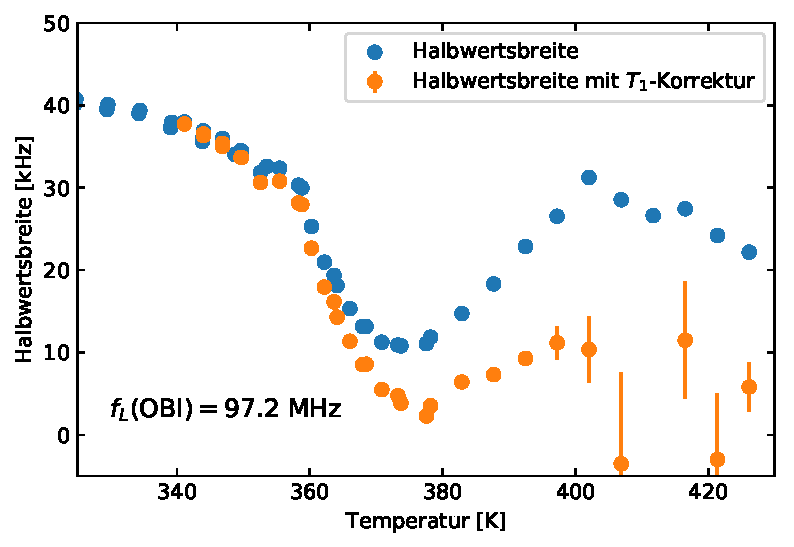
\includegraphics[width=.8\textwidth]{graphics/plot/fwhm_t1.pdf}
	\end{center}
	\caption{Halbwertsbreiten der OBI-Spektren in blau, mit der beschriebenen $T_1$-Korrektur in orange. Die gezeigten Unsicherheiten stammen aus den Unsicherheiten der $T_1$-Werte.} \label{fig:res:spek_fwhm_t1}
\end{figure}

Es ist zu erkennen, dass $T_1$ bei Temperaturen über $\SI{360}{\kelvin}$ einen großen Einfluss auf die Halbwertsbreite hat und die entsprechend angepassten Halbwertsbreiten deutlich geringere Werte aufweisen. Bei Temperaturen über $\SI{410}{\kelvin}$ können auch negative Halbwertsbreiten gefunden werden; diese sind aber aufgrund der hohen Schwankungen der $T_1$-Werte in diesem Temperaturbereich mit entsprechend hohen Unsicherheiten belegt. Eine präzisere Messung von $T_1$ würde eine Korrektur mit geringeren Unsicherheiten erlauben.




Es wurden die am OBI- und am Bruker-Spektrometer aufgenommenen Daten getrennt untersucht, da durch die unterschiedlichen Larmorfrequenzen abweichende Ergebnisse der theoretischen Kurven zu erwarten sind. Bei den Halbwertsbreiten wurde der $T_1$-Einfluss nach der beschriebenen Methode berücksichtigt.



Die aufgenommenen Spektren unterstützen eine biexponentielle Interpretation wie in \eqref{eqn:trans_relax} nur schwerlich, daher wurde lediglich der deutlich zu beobachtende Anteil des Zentralübergangs, $\Delta_c$ und $\omega_c^{(2)}$, für die entsprechenden FWHM- bzw. Schwer\-punkts-Da\-ten betrachtet. Für die $T_1$-Daten wird Formel \eqref{eqn:bpp} verwendet. Die Anpassung der Kurven wurde manuell durchgeführt.



Zunächst sollen die Daten des OBI-Spektrometers vergleichen werden. Bei den $T_1$-Werten soll erwähnt werden, dass die Werte bei hohen Temperaturen mit starken Unsicherheiten belegt sind (vgl. Abbildung \ref{fig:res:T_1}) -- entsprechende Indikatoren wurden hier für eine bessere Übersicht ausgelassen.

Für die Spektraldichte $J_\text{BPP}$ kann bei höheren Temperaturen, wie in Abbildung \ref{fig:res:theorie_j} zu sehen, mit dem Parameter $C_Q = \SI{3.6}{MHz}$ eine vergleichsweise gute Übereinstimmung für die Halbwertsbreiten und die Schwerpunkte erreicht werden. Zu tieferen Temperaturen gibt es jedoch gravierende Abweichungen. Für die stark ansteigenden Werte der Halbwertsbreite können anisotrope Effekte vermutet werden, deren Einfluss durch diese isotrope Theorie nicht abgedeckt wird und daher diesen Unterschied kreiert. Gründe für die Abweichungen der Schwerpunkte sind noch offen -- dieser Effekt wird jedoch gleichermaßen in experimentellen als auch simulierten Spektren beobachtet, was bedeutet, dass der Effekt vermutlich auf die von der Simulation berücksichtigten Wechselwirkungen eingeschränkt werden kann.
\begin{figure}
	\begin{center}
		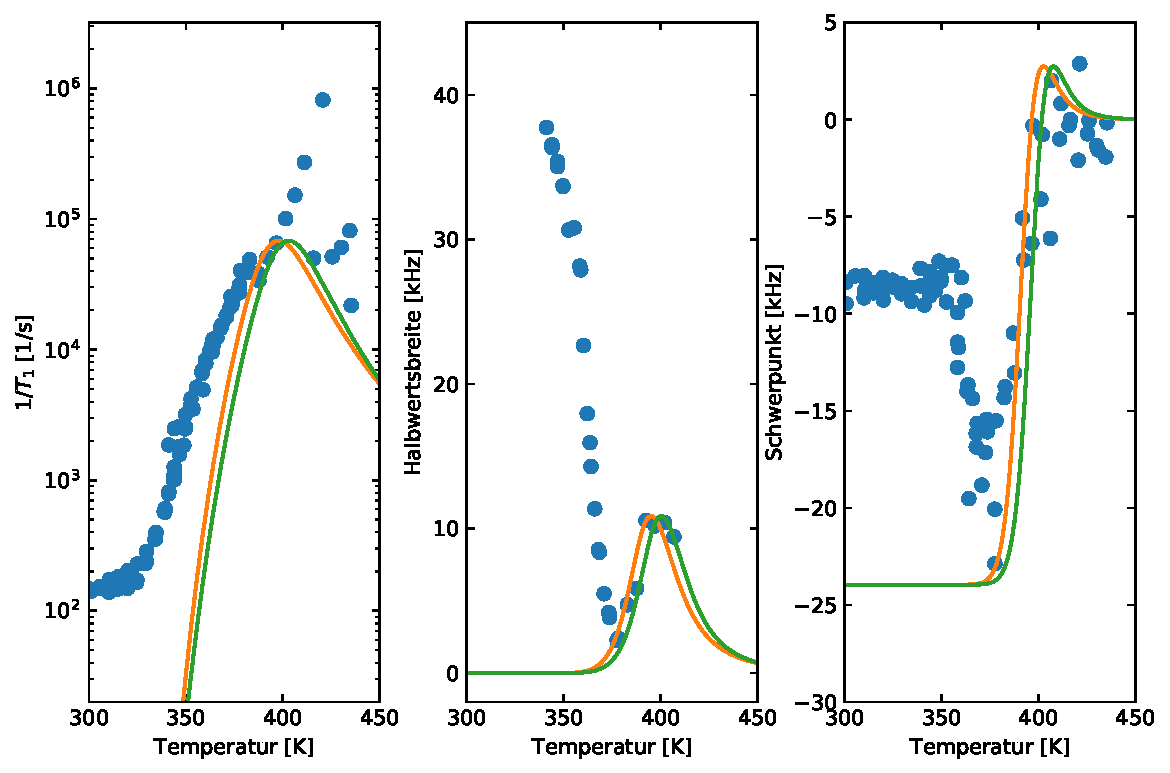
\includegraphics[width=.9\textwidth]{graphics/plot/OBI_J_02.pdf}
	\end{center}
	\caption{Vergleich von $T_1$, Halbwertsbreite und Schwerpunkt der OBI-Daten in blau. In orange die Theorie-Kurve mit Spektraldichte $J_\text{BPP}$ mit Parametern nach \cite{PIMENOV199793}, in grün mit Parametern nach \cite{crn_augsburg}.} \label{fig:res:theorie_j}
\end{figure}

Es kann eine grobe Vereinbarkeit der Theorie mit $T_1$-Werten im Maximum der Kurve erreicht werden, die Flanken unterscheiden sich jedoch deutlich. Da die Form der Theoriekurve mit der Spektraldichte $J_\text{BPP}$ unveränderlich ist, ist es schwerlich möglich, eine zufriedenstellende Übereinstimmung zu erreichen. Abhilfe schaffen könnten andere Spektraldichten -- dies soll im Folgenden untersucht werden.

Für die Spektraldichten $J_\text{CC}$ (Abbildung \ref{fig:res:theorie_j_cc}) und $J_\text{CD}$ (Abbildung \ref{fig:res:theorie_j_dc}) lagen die für die theoretische Berechnung der Schwerpunkte benötigten Imaginärteile $Q_\text{CC}$ und $Q_\text{CD}$ nicht vor, weswegen für diese auf die Spektraldichte $J_\text{BPP}$ zurückgegriffen wurde. Für die Schwerpunkte kann der Vergleich daher nur als grobe Idee verstanden werden.
\begin{figure}
	\begin{center}
		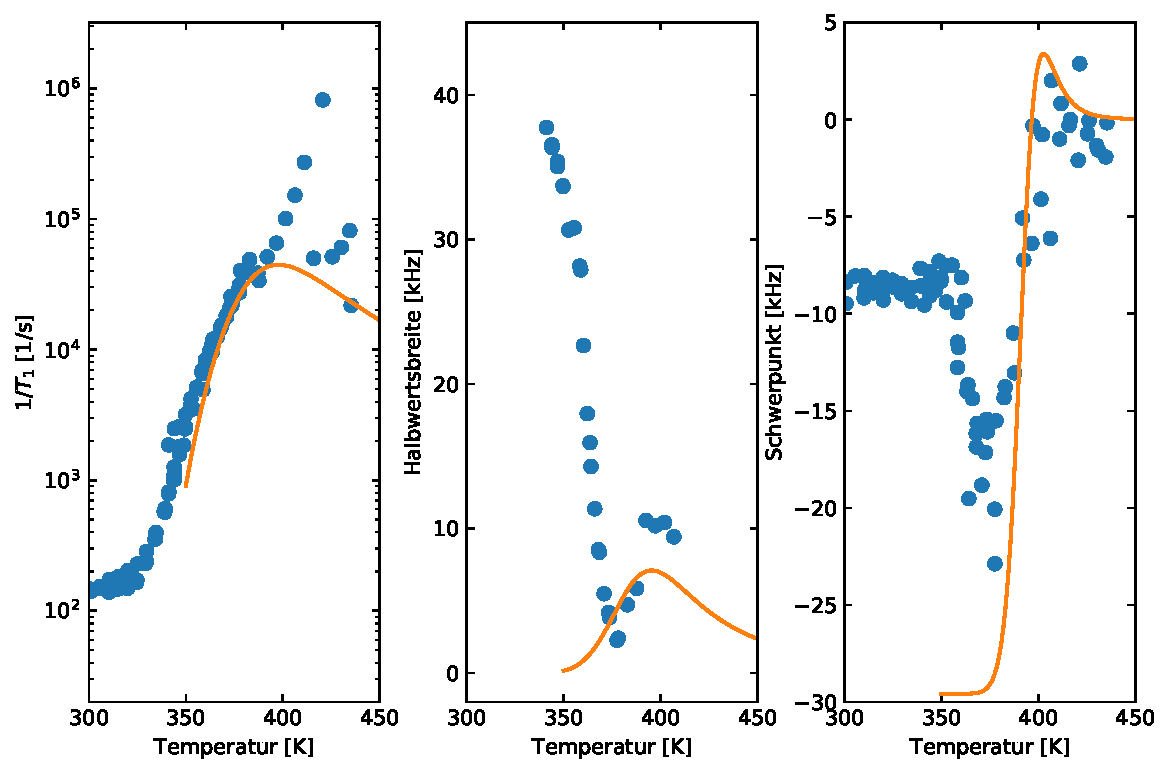
\includegraphics[width=.8\textwidth]{graphics/plot/OBI_J_cc_01.pdf}
	\end{center}
	\caption{Vergleich von $T_1$, Halbwertsbreite und Schwerpunkt der OBI-Daten in blau. In orange die Theoriekurve mit Spektraldichte $J_\text{CC}$ mit Parametern nach \cite{PIMENOV199793}.} \label{fig:res:theorie_j_cc}
\end{figure}
\begin{figure}
	\begin{center}
		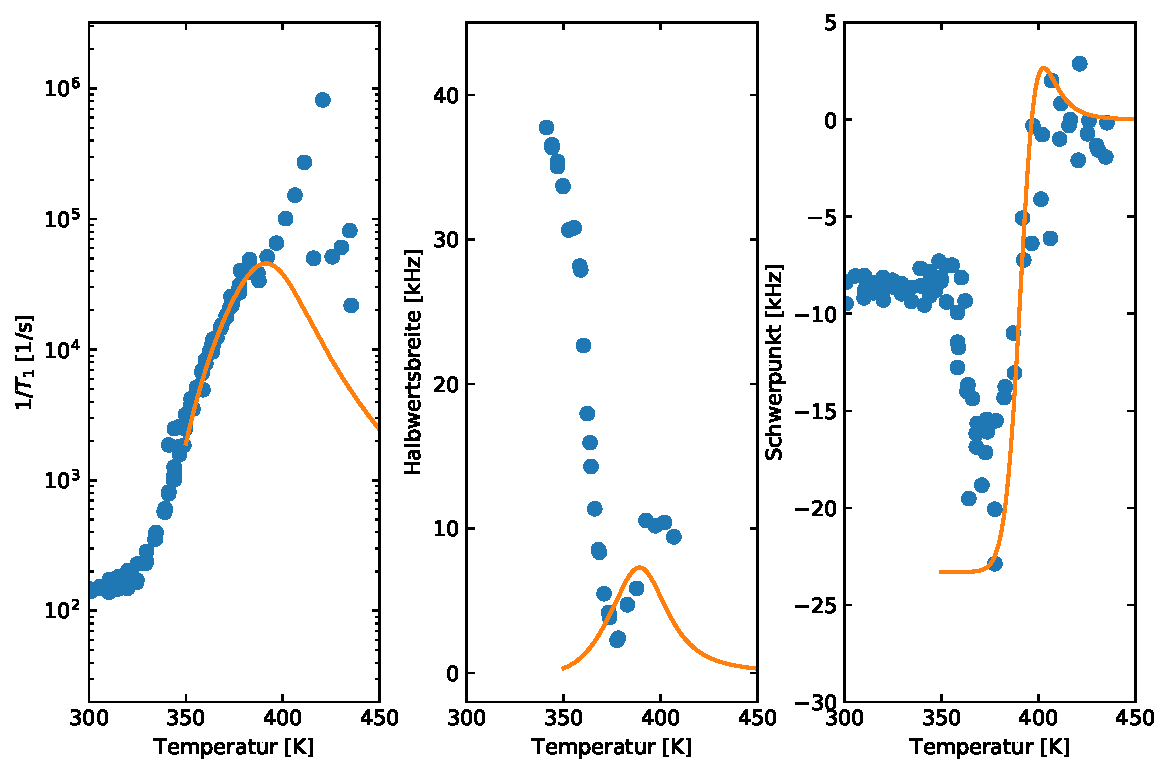
\includegraphics[width=.8\textwidth]{graphics/plot/OBI_J_dc_01.pdf}
	\end{center}
	\caption{Vergleich von $T_1$, Halbwertsbreite und Schwerpunkt der OBI-Daten in blau. In orange die Theorie-Kurve mit Spektraldichte $J_\text{CD}$ mit Parametern nach \cite{PIMENOV199793}.} \label{fig:res:theorie_j_dc}
\end{figure}

Für $J_\text{CC}$ und $J_\text{CD}$ können mit den Parametern $C_Q = \SI{4.0}{MHz}$ und $\alpha = \SI{0.6}{}$ bzw. $C_Q = \SI{3.6}{MHz}$ und $\gamma = \SI{0.46}{}$ gute Übereinstimmungen für $T_1$ beobachtet werden -- zumindest oberhalb einer Temperatur von etwa $\SI{350}{\kelvin}$. Für $J_\text{CD}$ scheint es zudem für Temperaturen über $\SI{400}{K}$ Abweichungen zu geben. Eine bessere Vereinbarkeit mit $T_1$-Werten kommt in beiden Fällen auf Kosten der vergleichsweise guten Übereinstimmungen für Halbwertsbreite und Schwerpunkt zustande, die mit $J_\text{BPP}$ erreicht werden konnten: Während für $J_\text{CC}$ die Schwerpunkte stark abweichen, ist dies bei $J_\text{CD}$ für die Halbwertsbreiten der Fall. Es bleibt festzuhalten, dass insgesamt eine gute Übereinstimmung mit der Theorie gezeigt werden konnte; es kann jedoch keine Spektraldichte besonders vorteilhaft hervorgehoben werden.

Für den Vergleich der Daten des Bruker-Spektrometers ist Ähnliches zu beobachten. Dabei fällt es hier aber schwerer, definitive Aussagen zu treffen, da der eingeschränkte Temperaturbereich nur einen bedingten Vergleich zulässt. Abbildung \ref{fig:res:theorie_bruker} zeigt die Daten zusammen mit Theoriekurven basierend auf der Spektraldichte $J_\text{BPP}$ mit dem Parameter $C_Q = \SI{3.45}{MHz}$. Dabei ist zu sehen, dass die Daten im gleichen Maße wie die OBI-Daten Übereinstimmungen und Unterschiede aufzeigen.
\begin{figure}
	\begin{center}
		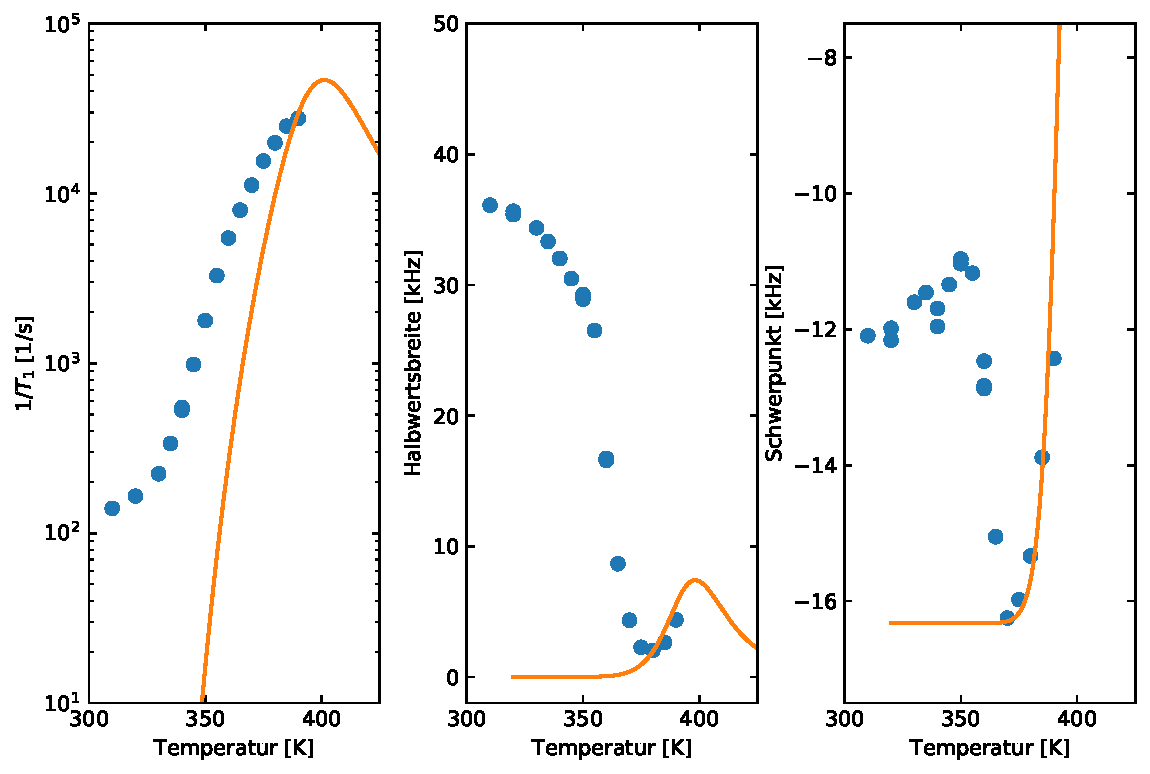
\includegraphics[width=.9\textwidth]{graphics/plot/Bruker_J_01.pdf}
	\end{center}
	\caption{Vergleich von $T_1$, Halbwertsbreite und Schwerpunkt der Bruker-Daten in blau. In orange die Theorie-Kurve mit Spektraldichte $J_\text{BPP}$ mit Parametern nach \cite{PIMENOV199793}.} \label{fig:res:theorie_bruker}
\end{figure}



\chapter{Zusammenfassung und Ausblick}


\printbibliography

\appendix
% Hier beginnt der Anhang, nummeriert in lateinischen Buchstaben
% \input{content/a_tensorundwignerd.tex}
% \input{content/b_qww2gedreht.tex}
% \input{content/c_pulsprogrammbruker.tex}

\backmatter


\cleardoublepage
\thispagestyle{empty}
\section*{Eidesstattliche Versicherung}
Ich versichere hiermit an Eides statt, dass ich die vorliegende Abschlussarbeit mit dem Titel \enquote{$^\text{87}$Rb-NMR Untersuchungen an Calciumrubidiumnitrat: Experiment und Simulation} selbstständig und ohne unzulässige fremde Hilfe erbracht habe.
Ich habe keine anderen als die angegebenen Quellen und Hilfsmittel benutzt, sowie wörtliche und sinngemäße Zitate kenntlich gemacht. 
Die Arbeit hat in gleicher oder ähnlicher Form noch keiner Prüfungsbehörde vorgelegen.

\vspace*{1cm}\noindent
\begin{center}
  \begin{tabular}{@{}p{0.4\textwidth}@{\hspace{0.15\textwidth}}p{0.4\textwidth}@{}}
  \rule{\linewidth}{0.25pt}& \rule{\linewidth}{0.25pt}\\
  Ort, Datum & Unterschrift
  \end{tabular}
\end{center}

\subsection*{Belehrung}
Wer vorsätzlich gegen eine die Täuschung über Prüfungsleistungen betreffende Regelung einer Hochschulprüfungsordnung verstößt, handelt ordnungswidrig.
Die Ordnungswidrigkeit kann mit einer Geldbuße von bis zu \SI[round-mode=places, round-precision=2]{50000}{€} geahndet werden. 
Zuständige Verwaltungsbehörde für die Verfolgung und Ahndung von Ordnungswidrigkeiten ist der Kanzler/die Kanzlerin der Technischen Universität Dortmund. 
Im Falle eines mehrfachen oder sonstigen schwerwiegenden Täuschungsversuches kann der Prüfling zudem exmatrikuliert werden \mbox{(\S\,63 Abs. 5 Hochschulgesetz --HG--).}

Die Abgabe einer falschen Versicherung an Eides statt wird mit Freiheitsstrafe bis zu 3 Jahren oder mit Geldstrafe bestraft.

Die Technische Universität Dortmund wird ggf.\ elektronische Vergleichswerkzeuge (wie z.\,B.\ die Software \enquote{turnitin}) zur Überprüfung von Ordnungswidrigkeiten in Prüfungsverfahren nutzen. \\[\baselineskip]

\noindent Die oben stehende Belehrung habe ich zur Kenntnis genommen.\\[1cm]
\begin{center}
\begin{tabular}{@{}p{0.4\textwidth}@{\hspace{0.15\textwidth}}p{0.4\textwidth}@{}}
\rule{\linewidth}{0.25pt}& \rule{\linewidth}{0.25pt}\\
Ort, Datum & Unterschrift
\end{tabular}
\end{center}

\end{document}
